\documentclass{article}
\usepackage[utf8]{inputenc}
\usepackage[T5]{fontenc}%Sử dụng tiếng Việt
\usepackage[fontsize=12pt]{scrextend}%Set fontsize
\usepackage[ paperheight=19.7cm,paperwidth=21cm,right=2cm,left=3cm,top=2cm,bottom=2.5cm]{geometry}%Chuẩn A4, căn lề phải, trái, trên, dưới
%\usepackage[a4paper, lmargin=0.1666\paperwidth, rmargin=0.1666\paperwidth, tmargin=0.1111\paperheight, bmargin=0.1111\paperheight]{geometry}
\usepackage{mathptmx}%Time New Roman
\usepackage{graphicx}%Thư viện chèn ảnh
\usepackage{float}%Set vị trí chèn ảnh
\usepackage{tikz}%Thư viện tạo khung hình
\usepackage{calc}%Thư viện tikz
\usepackage{indentfirst} %thư viện thụt đầu dòng
\renewcommand{\baselinestretch}{1.2}%giãn dòng 1.2
\setlength{\parskip}{6pt}%Setting after
\setlength{\parindent}{1cm} %set khoảng cách thụt đầu dòng mỗi đoạn
\usepackage{titlesec}%Thư viện setup các kiểu chữ
\setcounter{secnumdepth}{4} %4 heading
%titlespacing khoảng cách, titleformat format của nó
\titlespacing*{\section}{0pt}{0pt}{5pt}%Heading 1
\titleformat*{\section}{\fontsize{22pt}{0pt}\selectfont \bfseries \centering}

\titlespacing*{\subsection}{0pt}{10pt}{0pt}%Heading 2
\titleformat*{\subsection}{\fontsize{16pt}{0pt}\selectfont \bfseries}

\titlespacing*{\subsubsection}{0pt}{10pt}{0pt}%Heading 3
\titleformat*{\subsubsection}{\fontsize{13pt}{0pt}\selectfont \bfseries \itshape}

\titlespacing*{\paragraph}{0pt}{10pt}{0pt}%Heading 4
\titleformat*{\paragraph}{\fontsize{12pt}{0pt}\selectfont \itshape} %in nghiêng itshape

\renewcommand*\contentsname{MỤC LỤC}

\renewcommand{\figurename}{\fontsize{12pt}{0pt}\selectfont \bfseries Hình}
\renewcommand{\thefigure}{\thesection.\arabic{figure}}
\usepackage{caption}
\captionsetup[figure]{labelsep=space}
\renewcommand{\listfigurename}{DANH MỤC HÌNH VẼ}

\renewcommand{\tablename}{\fontsize{12pt}{0pt}\selectfont \bfseries Bảng}
\renewcommand{\thetable}{\thesection.\arabic{table}}
\captionsetup[table]{labelsep=space}
\renewcommand{\listtablename}{DANH MỤC BẢNG}

\usepackage{tabularx}
\newcolumntype{s}{>{\hsize=.4\hsize}X}
\newcolumntype{m}{>{\hsize=.8\hsize}X}
\newcolumntype{a}{>{\hsize=1.1\hsize}X}

\usepackage{longtable}
\usepackage{lipsum} % just for dummy text- not needed for a longtable

\usepackage{supertabular}

%file world là bản chuẩn, nên vào đó để xem nên set như thế nào
\begin{document}
\cleardoublepage
\thispagestyle{empty}
\begin{center}
\textbf{\fontsize{15pt}{0pt}\selectfont TRƯỜNG ĐẠI HỌC BÁCH KHOA HÀ NỘI}\\
\vspace{2.5cm}%Khoảng cách so với bên trên
%textbf in đậm
%\\ là xuống dòng
\textbf{\fontsize{25pt}{0pt}\selectfont ĐỒ ÁN TỐT NGHIỆP}\\
\hspace{10pt}\\
\textbf{\fontsize{23pt}{0pt}\selectfont Phần mềm đấu giá trực tuyến }  \vspace{1cm}\\
\textbf{\fontsize{14pt}{0pt}\selectfont NGUYỄN THỊ TRÀ }  \vspace{6pt}\\
\fontsize{13pt}{0pt}\selectfont tra.nt164200@sis.hust.edu.vn  \vspace{6pt}\\
\textbf{\fontsize{14pt}{0pt}\selectfont Chuyên ngành Kỹ thuật phần mềm }\vspace{8pt}\\
\begin{table}[H]
    \centering
    \begin{tabular}{l l l}
     \textbf{\fontsize{13pt}{0pt}\selectfont Giảng viên hướng dẫn:}& \fontsize{13pt}{0pt}\selectfont ThS.Nguyễn Tiến Thành \vspace{6pt}\\
     \textbf{\fontsize{13pt}{0pt}\selectfont Bộ môn:}& \fontsize{13pt}{0pt}\selectfont Kỹ thuật phần mềm \vspace{6pt}\\
      \textbf{\fontsize{13pt}{0pt}\selectfont Trường:}& \fontsize{13pt}{0pt}\selectfont Công nghệ Thông tin - Truyền thông
    \end{tabular}
\end{table}
\vspace{2.5cm}
\textbf{\fontsize{13pt}{0pt}\selectfont HÀ NỘI, 6/2022 }
\end{center}
\cleardoublepage
\section*{LỜI CAM KẾT}
\begin{table}[H]
    \begin{tabular}{l l l}
     \fontsize{13pt}{0pt}\selectfont Họ và tên sinh viên:& \fontsize{13pt}{0pt}\selectfont Nguyễn Thị Trà \vspace{6pt}\\
     \fontsize{13pt}{0pt}\selectfont Điện thoại liên lạc: 0332741666& \fontsize{13pt}{0pt}\selectfont Email:tra.nt164200@sis.hust.edu.vn \vspace{6pt}\\
     \fontsize{13pt}{0pt}\selectfont Lớp:CNTT02.03-K61& \fontsize{13pt}{0pt}\selectfont Hệ đào tạo: Kỹ sư chính quy
    \end{tabular}
\end{table}
Tôi – Nguyễn Thị Trà – cam kết Đồ án Tốt nghiệp (ĐATN) là công trình nghiên cứu của bản thân tôi dưới sự hướng dẫn của ThS. Nguyễn Tiến Thành. Các kết quả nêu trong ĐATN là trung thực, là thành quả của riêng tôi, không sao chép theo bất kỳ công trình nào khác. Tất cả những tham khảo trong ĐATN – bao gồm hình ảnh, bảng biểu, số liệu, và các câu từ trích dẫn – đều được ghi rõ ràng và đầy đủ nguồn gốc trong danh mục tài liệu tham khảo. Tôi xin hoàn toàn chịu trách nhiệm với dù chỉ một sao chép vi phạm quy chế của nhà trường.
\vspace{6pt}	

\hspace{6cm} Hà Nội, ngày    tháng    năm\\

\hspace{6.5cm} {Tác giả ĐATN}\\

\hspace{6.3cm} Họ và tên sinh viên\\

\hspace{6.5cm} Nguyễn Thị Trà

\newpage

\thispagestyle{empty}

\pagenumbering{arabic} %Đánh số theo thứ tự 1,2,3 ....
\section*{LỜI CẢM ƠN}
\addcontentsline{toc}{section}{\numberline {} LỜI CẢM ƠN}
\thispagestyle{empty}
Lời đầu tiên, Con cảm ơn Bố Mẹ, cảm ơn những người Anh Chị đã luôn yêu thương con hết lòng. Lúc mà con mệt mỏi nhất, bế tắc nhất, nơi con vẫn muốn tìm về là Gia đình, để con được xoa dịu tâm hồn đầy vết xước, tìm sự lắng nghe, chia sẻ để vững vàng bước tiếp trên con đường phía trước. Cuộc đời này dù là cả ngàn thử thách, thì chưa bao giờ con có ý định từ bỏ, hay chấp nhận buông tay. Vì con có một Gia đình luôn yêu thương, bên cạnh con vô điều kiện.
Tiếp theo em xin gửi lời cảm ơn sâu sắc đến ThS. Nguyễn Tiến Thành, trong thời gian làm đồ án Thầy đã hỗ trợ và chỉ dạy em rất nhiều điều. Em cảm ơn Thầy vì đã luôn đồng hành với em trong thời gian làm đồ án, đưa ra cho em những lời khuyên, những định hướng để xây dựng được một sản phẩm hoàn thiện nhất và có tính khoa học nhất trong quá trình làm việc. Em xin chân thành cảm ơn Thầy rất nhiều. \\
Một lời cảm ơn không thể thiếu đến những người bạn của tôi, đã cùng tôi đi qua những năm tháng đẹp nhất của Thanh xuân. Cảm ơn các bạn đã vẽ thêm những nét vẽ độc đáo trong Thanh xuân của tôi. \\
Và cuối cùng lời cảm ơn đến Bách Khoa, là cả những người bạn, người Thầy Cô đã cho tôi những năm tháng Thanh xuân rực rỡ và đáng nhớ nhất. Chỉ muốn nói rằng Bách Khoa à, tôi luôn tự hào khi nhắc đến Cậu, khi nói với ai đó rằng “Tôi là Người Bách Khoa” và hô to câu khẩu hiệu :\\
“Chúng ta là? …Sinh viên Bách Khoa\\
Chúng ta có? ….Sức trẻ và nghị lực\\
Chúng ta sống? …Hết mình vì tương lai.”\\
Cảm ơn Cậu nhé! Nhất định tôi sẽ thành công và bay thật xa đôi cánh tri thức mà Cậu đã chắp cho tôi 5 năm qua. \\
Cảm ơn 5 năm qua rất nhiều!
\cleardoublepage

\thispagestyle{empty}
\section*{TÓM TẮT ĐỒ ÁN}
\addcontentsline{toc}{section}{\numberline {} TÓM TẮT ĐỒ ÁN}
\thispagestyle{empty}
Hiện nay nhu cầu trao đổi, mua bán hàng hóa của người tiêu dùng phát triển không ngừng. Qua các giai đoạn phát triển của con người, xã hội thì các hình thức mua bán ngày càng đa dạng. Từ chợ, cửa hàng tạp hóa đến siêu thị, trung tâm thương mại lớn, và hiện nay thương mại điện tử đang chiếm tỷ lệ người dùng lớn trong nhu cầu mua sắm. \\
Để tăng thêm sự đa dạng trong cách thức mua sắm, ngoài các cửa hàng trên các sàn thương mại điện tử có mức giá cố định thì một số sàn khác nhằm tăng sức thu hút, cạnh tranh khi mua hàng của người tiêu dùng, đã tổ chức các buổi đấu giá trực tuyến để người tiêu dùng đưa ra giá, ai trả giá cao nhất thì được sở hữu sản phẩm. Hình thức này hiện nay rất được thu hút người tiêu dùng, kể cả nhóm người mua hàng và bán hàng.\\
Nhằm đáp ứng nhu cầu này cho người dùng thì trên thị trường có nhiều ứng dụng, website tổ chức các buổi đấu giá trực tuyến để người dùng có thể trao đổi, mua bán các sản phẩm như ebay.com, sohot.vn, lacvietauction.vn….Tuy nhiên ebay phổ biến trên thế giới, nhưng không được phổ biến ở Việt Nam, chỉ dùng tiếng Anh và các ngôn ngữ khác. Việc thanh toán và vận chuyển về Việt Nam cũng rất khó khăn vì khoảng cách quá xa. Còn sohot.vn thì chủ yếu là đồ dùng nội thất, mặt hàng không đa dạng, giao diện cũng không được thân thiện với người dùng hiện nay.\\ 
Chính vì vậy, ở đồ án tốt nghiệp này em đã quyết định xây dựng một website đấu giá trực tuyến. Website nhằm đáp ứng một số mục đích cơ bản như phù hợp với người Việt Nam hơn, có đầy đủ chức năng cần thiết và mang lại trải nghiệm tốt hơn cho người dùng. Người dùng có thể tổ chức, tham gia các phiên đấu giá trên hệ thống, quản trị viên cũng được cung cấp một hệ thống quản lý toàn bộ website. Ngoài ra để đáp ứng thêm một nhóm người Nhật Bản tại Việt Nam, em cũng định hướng xây dựng website có thể chuyển đổi  qua lại giữa tiếng Nhật và tiếng Việt.
\cleardoublepage

\addtocontents{toc}{\protect\thispagestyle{empty}}
\tableofcontents %Tạo mục lục tự động
\thispagestyle{empty}
\cleardoublepage

%\pagenumbering{roman}%Đánh số theo thứ tự la mã

{%
\let\oldnumberline\numberline%
\renewcommand{\numberline}{\figurename~\oldnumberline}%
\listoffigures%
} %Tạo danh mục hình vẽ tự động
\addcontentsline{toc}{section}{\numberline {} DANH MỤC HÌNH VẼ}
\cleardoublepage

%Tạo danh mục bảng biểu tự động
{%
\let\oldnumberline\numberline%
\renewcommand{\numberline}{\tablename~\oldnumberline}%
\listoftables%
}
\addcontentsline{toc}{section}{\numberline {} DANH MỤC BẢNG}
\cleardoublepage

\section*{DANH MỤC CÁC TỪ VIẾT TẮT}
\addcontentsline{toc}{section}{\numberline{} DANH MỤC CÁC TỪ VIẾT TẮT}
\begin{table}[H]
    \centering
    \begin{tabular}{p{.20\textwidth} l p{.30\textwidth}}
        \fontsize{13pt}{0pt}\selectfont \bfseries API&\fontsize{13pt}{0pt}\selectfont Application Programming Interface
        \vspace{6pt}\\
        &\fontsize{13pt}{0pt}\selectfont Giao diện lập trình ứng dụng\vspace{8pt}\\
        \fontsize{13pt}{0pt}\selectfont \bfseries C2C&\fontsize{13pt}{0pt}\selectfont Consumer To Consumer
        \vspace{6pt}\\
        &\fontsize{13pt}{0pt}\selectfont Người tiêu dùng tới người tiêu dùng\vspace{8pt}\\
        \fontsize{13pt}{0pt}\selectfont \bfseries HTML&\fontsize{13pt}{0pt}\selectfont HyperText Markup Language
        \vspace{6pt}\\
        &\fontsize{13pt}{0pt}\selectfont Ngôn ngữ đánh dấu siêu văn bản\vspace{8pt}\\
        \fontsize{13pt}{0pt}\selectfont \bfseries DOM&\fontsize{13pt}{0pt}\selectfont Document Object Model
        \vspace{6pt}\\
        &\fontsize{13pt}{0pt}\selectfont Mô hình đối tượng tài liệu bản\vspace{8pt}\\
        \fontsize{13pt}{0pt}\selectfont \bfseries TCP&\fontsize{13pt}{0pt}\selectfont Transmission Control Protocol
        \vspace{6pt}\\
        &\fontsize{13pt}{0pt}\selectfont Giao thức điều khiển truyền vận\vspace{8pt}\\
        \fontsize{13pt}{0pt}\selectfont \bfseries CSRF&\fontsize{13pt}{0pt}\selectfont Cross Site Request Forgery
        \vspace{6pt}\\
        &\fontsize{13pt}{0pt}\selectfont Kỹ thuật tấn công giả mạo vận\vspace{8pt}\\
        \fontsize{13pt}{0pt}\selectfont \bfseries ĐATN&\fontsize{13pt}{0pt}\selectfont Đồ án tốt nghiệp\vspace{8pt}\\
        \fontsize{13pt}{0pt}\selectfont \bfseries REST&\fontsize{13pt}{0pt}\selectfont REpresentational State Transfer\vspace{8pt}\\
        \fontsize{13pt}{0pt}\selectfont \bfseries PHP&\fontsize{13pt}{0pt}\selectfont Hypertext Preprocessor\vspace{8pt}\\
    \end{tabular}
\end{table}
\cleardoublepage

\section*{DANH MỤC THUẬT NGỮ}
\addcontentsline{toc}{section}{\numberline{} DANH MỤC THUẬT NGỮ}
\begin{table}[H]
    \centering
    \begin{tabular}{p{.23\textwidth} l p{.30\textwidth}}
        \fontsize{13pt}{0pt}\selectfont \bfseries Admin&\fontsize{13pt}{0pt}\selectfont Quản trị viên\vspace{8pt}\\
        \fontsize{13pt}{0pt}\selectfont \bfseries Server&\fontsize{13pt}{0pt}\selectfont Máy chủ\vspace{8pt}\\
        \fontsize{13pt}{0pt}\selectfont \bfseries Client&\fontsize{13pt}{0pt}\selectfont Máy khách\vspace{8pt}\\
        \fontsize{13pt}{0pt}\selectfont \bfseries Black box&\fontsize{13pt}{0pt}\selectfont Kiểm thử hộp đen\vspace{8pt}\\
        \fontsize{13pt}{0pt}\selectfont \bfseries
        \fontsize{13pt}{0pt}\selectfont \bfseries Backend&\fontsize{13pt}{0pt}\selectfont Lập trình máy chủ hệ thống\vspace{8pt}\\
        Fontend&\fontsize{13pt}{0pt}\selectfont Lập trình máy khách hệ thống\vspace{8pt}\\
        \fontsize{13pt}{0pt}\selectfont \bfseries Database&\fontsize{13pt}{0pt}\selectfont Cơ sở dữ liệu\vspace{8pt}\\
        \fontsize{13pt}{0pt}\selectfont \bfseries Chat&\fontsize{13pt}{0pt}\selectfont Nhắn tin\vspace{8pt}\\
        \fontsize{13pt}{0pt}\selectfont \bfseries Realtime&\fontsize{13pt}{0pt}\selectfont Thời gian thực\vspace{8pt}\\
        \fontsize{13pt}{0pt}\selectfont \bfseries Component&\fontsize{13pt}{0pt}\selectfont Thành phần\vspace{8pt}\\
        \fontsize{13pt}{0pt}\selectfont \bfseries Blade&\fontsize{13pt}{0pt}\selectfont Template engine đơn giản\vspace{8pt}\\
    \end{tabular}
\end{table}
\cleardoublepage

\section*{CHƯƠNG 1 GIỚI THIỆU ĐỀ TÀI}
\addcontentsline{toc}{section}{\numberline{}CHƯƠNG 1 GIỚI THIỆU ĐỀ TÀI}
\setcounter{section}{1}
\subsection{Đặt vấn đề}
Trong thời kỳ phát triển như ngày nay, nhu cầu mua bán, trao đổi hàng hóa của con người ngày càng tăng cao. Để thu hút được khách hàng thì các nhà kinh doanh không ngừng thay đổi cách thức, dịch vụ bán hàng. Nắm bắt được tâm lý của khách hàng, nhiều nhà kinh doanh ngoài việc bán các mặt hàng giá cố định thì đã tổ chức nhiều phiên đấu giá để kích thích sự cạnh tranh khi mua hàng của người tiêu dùng. Việc này tạo hiệu ứng rất tốt đối với người dùng, họ được tự mình định giá cho sản phẩm của mình, may mắn hơn thì mua được sản phẩm với giá rẻ hơn ngoài thị trường mà chất lượng không hề rẻ. \\
Tuy nhiên khi tổ chức các phiên đấu giá truyền thống thì phát sinh nhiều vấn đề như: thủ tục tổ chức, hội trường, số lượng người tham gia, thời gian bị giới hạn. Bên cạnh đó sàn đấu giá truyền thống thường chỉ đấu giá những sản phẩm có giá trị lớn như nhà đất, đồ cổ quý hiếm….Vì vậy các sản phẩm có giá trị nhỏ hơn khó tiếp cận với khách hàng. Ngoài ra khi số lượng phiên đấu giá lớn dần thì việc quản lý trở nên rất khó khăn và mất thời gian. \\
Thêm vào đó thương mại điện tử đang ngày càng phát triển và dần trở thành xu hướng tất yếu của thị trường. Bởi vậy, một website đấu giá trực tuyến ra đời sẽ góp phần giải quyết được các vấn đề nói trên. Khi tổ chức một phiên đấu giá trực tuyến thì người bán không mất chi phí thuê hội trường, số lượng người tham gia, thời gian có thể linh động dễ dàng. Số lượng sản phẩm của phiên đấu giá cũng đa dạng hơn, dễ tiếp cận với số lượng lớn người dùng hơn. Đặc biệt việc quản lý, theo dõi các phiên đấu giá dễ dàng và tiết kiệm thời gian hơn.\\
Tuy nhiên theo khảo sát của em về thị trường Việt Nam hiện nay, có rất ít website đấu giá trực tuyến và các phiên đấu giá thường hay giới hạn nhóm sản phẩm. Còn các sàn đấu giá nước ngoài thì không phù hợp với người Việt Nam, do vấn đề ngôn ngữ, vận chuyển, đổi trả hàng.\\ 
Nhận thấy cả lợi ích và hạn chế của những sản phẩm hiện có. Em quyết định đặt mục tiêu cho đồ án là xây dựng một website đấu giá trực tuyến với mô hình C2C. 
\subsection{Mục tiêu và phạm vi đề tài}
Trên thị trường hiện nay có rất nhiều ứng dụng, website tổ chức các phiên đấu giá trực tuyến ở cả Việt Nam và nước ngoài. Phổ biến nhất phải kể đến là ebay.com  ở thị trường nước ngoài, sohot.vn, lacvietauction.vn của Việt Nam. \\
Ebay.com thì phổ biến trên nhiều quốc gia, sản phẩm đa dạng, có nhiều thương hiệu nổi tiếng, nhưng hiện nay nó không có bản tiếng Việt, cũng không được ưa chuộng tại Việt Nam vì vấn đề là nơi bán quá xa, quá trình vận chuyển vừa mất thời gian, vừa không đảm bảo được trên quãng đường dài như thế thì các sản phẩm dễ vỡ có còn được nguyên vẹn hay không, rồi vấn đề thất lạc sản phẩm, trả hàng nếu muốn cũng rất khó khăn. Còn ở Việt Nam thì có sohot.vn, khi muốn đấu giá trên sàn này thì cần phải đăng ký qua 5giay.vn, giao diện rất khó sử dụng, bên cạnh đó trên sohot.vn chỉ có một số mặt hàng chủ yếu liên quan đến nội thất gia đình. Ngoài ra có sàn đấu giá lacvietauction.vn cũng rất được ưa chuộng tại Việt Nam, tuy nhiên sàn đấu giá này chủ yếu trưng bày, đấu giá  các sản phẩm có giá trị lớn như căn hộ, đất đai, xe ô tô….việc này cũng gây khó khăn cho nhóm người muốn bán những sản phẩm, đồ dùng có giá trị nhỏ hơn. \\
Do vậy ở đồ án tốt nghiệp này em muốn xây dựng một website cung cấp cho người dùng Việt Nam trải nghiệm tốt hơn, giao diện dễ sử dụng hơn. Bên cạnh đó để đáp ứng nhiều nhóm người dùng hơn thì phần mềm sẽ không giới hạn hay yêu cầu là chỉ bán một mặt hàng nhất định và không ràng buộc mặt hàng đó phải có giá trị thấp nhất là bao nhiêu. Bên cạnh đó để thuận tiện cho việc liên lạc trao đổi giữa các người dùng với nhau thì phần mềm cũng cung cấp cho người dùng ứng dụng chat realtime để liên lạc trao đổi giữa các bên khi cần. \\
Ngoài ra vì muốn hướng tới thêm một nhóm người Nhật Bản tại Việt Nam (hoặc nhóm có nhu cầu sử dụng tiếng Nhật) có nhu cầu bán lại đồ đã qua sử dụng với giá rẻ thì ứng dụng cung cấp việc chuyển đổi giữa tiếng Việt và tiếng Nhật cũng góp phần nâng cao trải nghiệm người dùng. 
\subsection{Định hướng giải pháp}
Để xây dựng hệ thống sàn đấu giá theo mục tiêu đề tài như đã trình bày ở trên, em định hướng xây dựng đề tài trên nền tảng web cho cả người dùng và người quản trị hệ thống. \\
Công nghệ sử dụng gồm có: ReactJs cho ứng dụng web, PHP framework Laravel cho Server. Mô hình sử dụng: Client - Server, kiến trúc sử dụng MVC (Model - View - Controller). Để xây dựng chức năng chat realtime đồ án sẽ sử dụng thư viện Socket.IO. Socket.IO giúp các bên kết nối với nhau, truyền dữ liệu ngay lập tức thông qua Server trung gian. Socket.IO với đặc trưng là dễ sử dụng nên rất được ưa chuộng bởi các lập trình viên, hỗ trợ  nhiều công nghệ realtime như WebSocket, Flash Socket, AJAX long-polling…\\
Mô hình sử dụng cho đồ án là Mô hình Client  - Server, là loại mô hình mà máy chủ (Server) sẽ lưu trữ các tài nguyên, quản lý,  xử lý các yêu cầu mà khách hàng tương tác trên màn hình và trả ra kết quả trên màn hình cho khách hàng. Client  - Server là mô hình mà một hay nhiều máy khách (Client) gửi yêu cầu đến máy chủ trung tâm. Mô hình Client - Server được sử dụng trong nhiều ứng dụng hiện nay như ứng dụng web hay ứng dụng di động. Client-Server chỉ mang đặc điểm của phần mềm mà không hề liên quan đến phần cứng, dễ sử dụng, dễ bảo trì, tái sử dụng, hỗ trợ người dùng nhiều dịch vụ đa dạng và sự tiện dụng bởi khả năng truy cập từ xa. Vì vậy đồ án lựa chọn mô hình này khi xây dựng ứng dụng cho Client, một cho trình duyệt web và một ứng dụng sẽ được cài đặt trên server để phục vụ cho ứng dụng Client thông qua lời gọi RESTful API. \\
Bên cạnh đó đồ án lựa chọn kiến trúc MVC (Model-View-Controller). Một kiến trúc khá phổ biến và được sử dụng nhiều trên các ứng dụng web ngày nay. Kiến trúc MVC đơn giản, phân chia ứng dụng thành nhiều lớp dễ sử dụng, dễ triển khai và bảo trì. Phần hiển thị ở Client như là View, còn Server gắn với Model và Controller trong kiến trúc.\\
Tóm lại, định hướng phát triển đề tài được triển khai như sau: Sử dụng Backend với Ngôn ngữ PHP framework Laravel, sử dụng thư viện ReactJs để xây dựng view hiển thị trên ứng dụng web, để có được chức năng chat realtime thì sử dụng thư viện Socket.IO, hệ quản trị cơ sở dữ liệu là MySQL. \\
Về công nghệ sử dụng đồ án sẽ trình bày chi tiết hơn trong Chương 3.
\subsection{Bố cục đồ án}
Phần còn lại của báo cáo đồ án tốt nghiệp này được chia làm sáu phần, với nội dung các chương như sau: \\
Chương 2 sẽ tập trung vào việc khảo sát hiện trạng thực tế hiện nay, đánh giá ưu nhược điểm của các sản phẩm đã có trên thị trường. Từ đó đưa ra những yêu cầu mà người dùng cần để xây dựng các chức năng cơ bản phù hợp với yêu cầu đó. Trong Chương 2 này đồ án cũng sẽ trình bày chi tiết về quy trình nghiệp vụ, đặc tả những chức năng chính của website. Cuối cùng là phân tích, đánh giá về các yêu cầu chức năng, phi chức năng mà đồ án đã đạt được và chưa đạt được.\\
Tiếp theo, Chương 3 trình bày về công nghệ sử dụng trong suốt đồ án . Bao gồm các cơ sở lý thuyết cơ bản về công nghệ đó và lý giải tại sao công nghệ được lựa chọn cho đồ án. \\
Chương 4 sẽ trình bày chi tiết về quá trình thiết kế kiến trúc, giao diện, lớp, cơ sở dữ liệu; chương này còn nêu lên quá trình xây dựng, kết quả đạt được và quá trình kiểm thử phần mềm cho toàn bộ đồ án này. Việc lựa chọn kiến trúc MVC, hay sử dụng hệ quản trị cơ sở dữ liệu MySQL cũng sẽ được trình bày chi tiết tại chương này. Phần kiểm thử bao gồm cả kiểm thử tự động và kiểm thử hộp đen các chức năng quan trọng của đồ án. Cuối cùng là kế hoạch triển khai dự án trên thực tế thì có những vấn đề gì cần chú ý, các thông số liên quan.\\
Những đóng góp của đồ án sẽ được trình bày trong chương 5. Ở chương này sẽ trình bày những đóng góp nổi bật của đồ án như (i) chat realtime giữa các người dùng trên website; (ii) tìm kiếm thông tin sản phẩm theo một số keyword nổi bật như tên phiên đấu giá, giá khởi điểm, thời gian bắt đầu, thời gian kết thúc; (iii) website cho phép người dùng đánh giá sản phẩm khi nhận được hàng; (iv) cung cấp hệ thống quản lý website dành cho Admin.\\
Cuối cùng, chương 6 sẽ là những kết luận và kết quả cuối cùng mà đồ án này đạt được. Phần này sẽ tổng kết, đánh giá những điều đã làm được, chưa làm được, những đóng góp chính của em trong đồ án và các định hướng phát triển trong tương lai để sản phẩm được hoàn thiện hơn. 
\newpage%kết thúc 1 chương

\section*{CHƯƠNG 2 GIỚI THIỆU ĐỀ TÀI}
\addcontentsline{toc}{section}{\numberline{}CHƯƠNG 2 GIỚI THIỆU ĐỀ TÀI}
\setcounter{section}{2}
\setcounter{subsection}{0}
\subsection{Khảo sát hiện trạng}
Hiện nay phần lớn các sàn đấu giá trực tuyến ở Việt Nam thì chủ yếu tập trung vào một nhóm khách hàng chủ yếu, hoặc nhóm sản phẩm chủ yếu. Còn sàn đấu giá trực tuyến ở nước ngoài thì không được sử dụng phổ biến tại Việt Nam vì một số vấn đề (i) quá xa, (ii) vận chuyển mất thời gian….\\
Dưới đây đồ án sẽ trình bày những ưu nhược điểm của một số sàn đấu giá trực tuyến phổ biến hiện nay ở cả Việt Nam và trên thế giới.
%\begin{table}[]
    %\centering
    \tablehead{%
    \hline
    \bfseries Sàn đấu giá & \bfseries Ưu điểm &  \bfseries Nhược điểm\\
    \hline}
    \tabletail{\hline}
    \topcaption{Khảo sát và đánh giá các sàn đấu giá trực tuyến hiện nay}
    \label{bang21}
    \begin{supertabular}{| p{.20\textwidth} | p{.30\textwidth} | p{.415\textwidth} |} 
        ebay.com &  ebay.com có sản phẩm đa dạng, phổ biến trên nhiều quốc gia, giao diện thân thiện với người dùng.
        ebay.com có hầu hết chức năng của một sàn đấu giá chuyên nghiệp.
        &  ebay.com không được phổ biến ở Việt Nam; không có chuyển đổi thành tiếng Việt; không tìm kiếm phiên đấu giá theo thời gian; không cho phép nhắn tin với người dùng khác.\\\hline
        sohot.vn &  sohot.vn liên kết với website 5giay.vn, phù hợp với người dùng Việt Nam có nhu cầu về nội thất gia đình.&  sohot.vn có giao diện không thân thiện, khó sử dụng; website chủ yếu bán sản phẩm nội thất gia đình; khi đăng ký phải thông qua 5giay.vn; chỉ tìm kiếm theo tên sản phẩm; không có đánh giá sản phẩm và không cho phép nhắn tin với người dùng khác.\\\hline
        lacvietauction.vn & lacvietauction.vn có giao diện dễ sử dụng; đảm bảo các tài khoản đăng ký mua bán là chính chủ nên việc xác minh tài khoản thực hiện rất chặt chẽ. & lacvietauction.com chỉ mua bán, đấu giá các sản phẩm có giá trị tương đối lớn như nhà đất, xe ô tô cũ…; chỉ tìm kiếm theo tên của từng nhóm sản phẩm; không có đánh giá sản phẩm; không cho phép nhắn tin với các người dùng khác .\\\hline
    \end{supertabular}\\
% \end{table}
\\
Về tổng thể các sàn đấu giá này giới hạn nhóm người dùng, nhóm sản phẩm mua bán; bỏ qua tìm kiếm phiên đấu giá theo thời gian; không cho phép nhắn tin với người dùng khác; hoặc sàn đấu giá nước ngoài thì không phù hợp với người Việt Nam. Chính vì những nhược điểm này, website đấu giá trực tuyến mà đồ án xây dựng sẽ cố gắng khắc phục những nhược điểm nói trên, bổ sung thêm các chứng năng khác nhằm phục vụ tốt hơn nhu cầu của người Việt Nam và một bộ phận người Nhật Bản ở Việt Nam.\\
Website sẽ bao gồm ba đối tượng chính là quản trị viên, người bán và người mua. Quản trị viên có nhiệm vụ quản lý hệ thống bao gồm việc phê duyệt phiên đấu giá; quản lý người dùng; thêm, sửa, xóa loại sản phẩm, thương hiệu, tin tức, slide của website. Người bán sẽ tạo phiên đấu giá về sản phẩm muốn bán. Trong trường hợp người bán có thắc mắc về quá trình tạo phiên đấu giá thì có thể liên lạc với Admin hoặc đọc hướng dẫn tạo phiên đấu giá ở mục tin tức trên Website. Còn người mua thì có thể tham gia các phiên đấu giá đang diễn ra, trả giá cho sản phẩm đó. Khi phiên đấu giá kết thúc, người mua nào đưa ra mức giá cao nhất sẽ được người bán chấp nhận giá và thực hiện giao hàng. Khi người mua nhận được hàng, thực hiện xác nhận và đánh giá sản phẩm, khi đó phiên đấu giá cập nhật trạng thái giao hàng thành công.\\
Mục đích cuối cùng là tạo ra một Website có đầy đủ các chức năng cần thiết của một sàn đấu giá trực tuyến và giải quyết các vấn đề còn thiếu của các sàn đấu giá nêu trên.
\subsection{Tổng quan chức năng}
\subsubsection{Biểu đồ use case tổng quan}
\begin{figure}[H]
    \centering
    \includegraphics[width=11.4cm,height=13.1cm]{images/uc tổng quan.png}
    \caption{Biểu đồ usecase Tổng quan}
    \label{hinh21}
\end{figure}
Website đấu giá trên gồm 3 tác nhân chính:\\ 
Khách: Là người dùng chưa có tài khoản, người dùng này có thể (i) xem, đọc tin tức; (ii) liên lạc với Admin qua email; (iii) xem thông tin phiên đấu giá trên hệ thống nhưng không thể bình luận hay trả giá. Để có thể sử dụng các chức năng của website thì khách phải tạo tài khoản và đăng nhập.\\
Người dùng: Là người đã có tài khoản. Người dùng này đăng nhập để sử dụng các chức năng của website. \\
Quản trị viên: Là người quản lý, vận hành website, có thể quản lý người dùng, phiên đấu giá, loại sản phẩm, thương hiệu, tin tức, slide của website. \\
Website đấu giá trực tuyến cung cấp cho người dùng những chức năng cơ bản như (i) tạo phiên đấu giá, (ii) tham gia đấu giá, (iii) bình luận, (iv) yêu thích, (v) đánh giá sản phẩm, (vi) nhắn tin với người dùng khác, (vii) tìm kiếm phiên đấu giá; (viii) quản lý phiên đấu giá của mình tổ chức như chỉnh sửa, xóa phiên đấu giá chưa được duyệt, chấp nhận giá của người trả giá cao nhất khi phiên đấu giá kết thúc, xác nhận đã giao hàng.\\
Về phía quản trị viên có thể chấp nhận hay từ chối phiên đấu giá mà người dùng tạo, có thể xóa tài khoản người dùng không còn hoạt động. Quản trị viên cũng quản lý việc thêm, sửa, xóa danh sách các loại sản phẩm, thương hiệu, tin tức, slide hiển thị trên website.
\subsubsection{Biểu đồ use case phân rã Quản lý người dùng}
\begin{figure}[H]
    \centering
    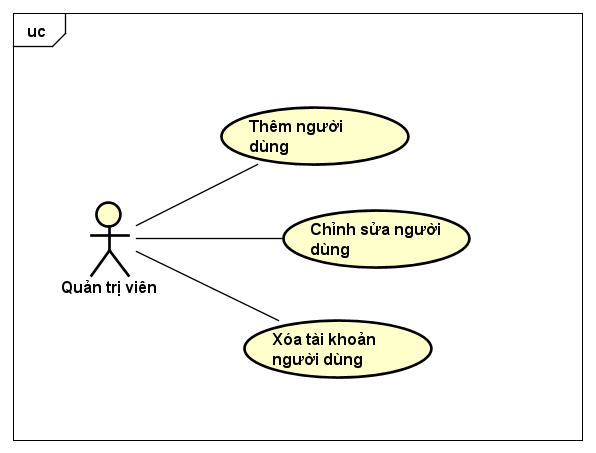
\includegraphics[width=11.4cm,height=8.67cm]{images/uc quản lý người dùng.png}
    \caption{Biểu đồ usecase Quản lý người dùng}
    \label{hinh22}
\end{figure}
Hình \ref{hinh22} mô tả chức năng Quản lý người dùng. Quản trị viên có thể thêm, chỉnh sửa những tài khoản do Admin thêm, xóa tài khoản không còn hoạt động nữa.
\subsubsection{Biểu đồ use case phân rã Quản lý phiên đấu giá}
\begin{figure}[H]
    \centering
    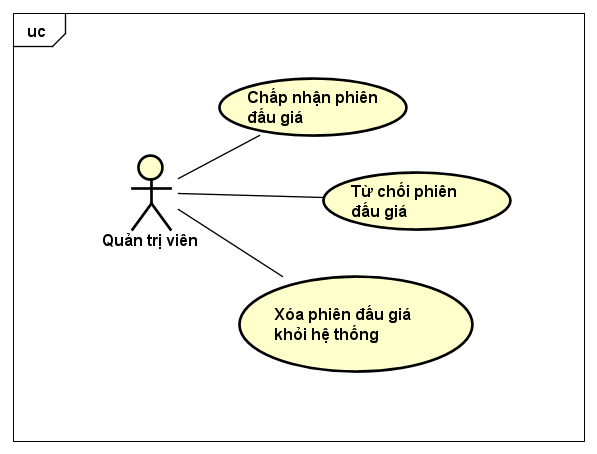
\includegraphics[width=11.4cm,height=8.67cm]{images/uc quản lý phiên đấu giá.png}
    \caption{Biểu đồ usecase Quản lý phiên đấu giá}
    \label{hinh23}
\end{figure}
Hình \ref{hinh23} mô tả chức năng Quản lý phiên đấu giá. Với chức năng này thì sau khi Người dùng tạo phiên đấu giá, phía Quản trị viên sẽ đánh giá phiên đấu giá đó đủ tiêu chuẩn để duyệt hay chưa. Nếu phiên đấu giá có thông tin không đầy đủ, chính xác thì Quản trị viên có quyền từ chối phiên đấu giá đó và hệ thống sẽ gửi thông báo cho Người tạo phiên đấu giá. Nếu phiên đấu giá được quản trị viên chấp nhận thì hệ thống sẽ cập nhật trạng thái và hiển thị công khai trên website. Với những phiên đấu giá đã được xác nhận giao hàng thành công thì Quản trị viên có thể xóa khỏi hệ thống.
\subsubsection{Biểu đồ use case phân rã Tạo phiên đấu giá}
\begin{figure}[H]
    \centering
    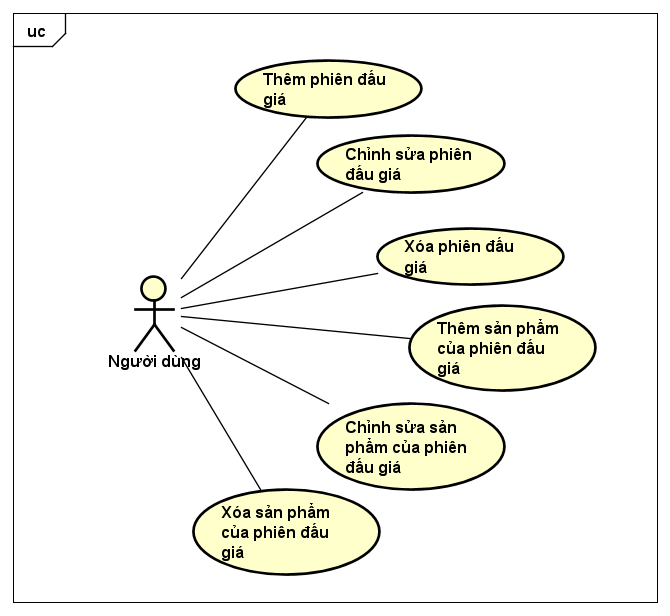
\includegraphics[width=11.4cm,height=10.49cm]{images/uc tạo phiên đấu giá.png}
    \caption{Biểu đồ usecase Tạo phiên đấu giá}
    \label{hinh24}
\end{figure}
Hình \ref{hinh24} mô tả chức năng Tạo phiên đấu giá của Người dùng. Người dùng có thể thêm mới một phiên đấu giá và thêm sản phẩm cho phiên đấu giá đó. Với những phiên đấu giá chưa được duyệt thì Người dùng có thể chỉnh sửa, xóa sản phẩm và phiên đấu giá đó.
\subsubsection{Biểu đồ use case phân rã Tìm kiếm thông tin}
\begin{figure}[H]
    \centering
    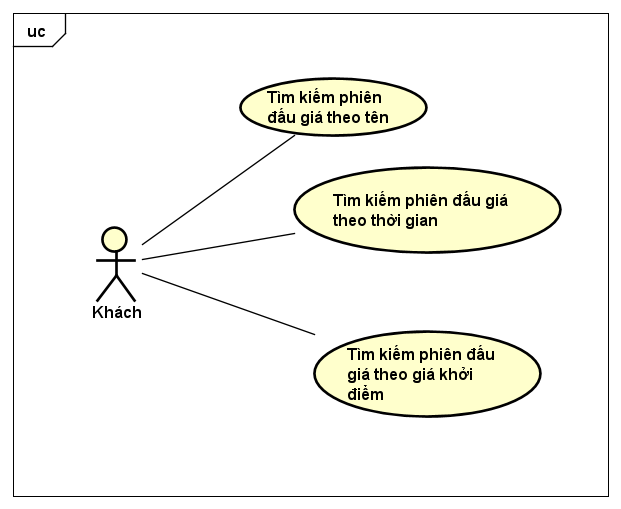
\includegraphics[width=11.4cm,height=9.35cm]{images/uc tìm kiếm thông tin.png}
    \caption{Biểu đồ usecase Tìm kiếm thông tin}
    \label{hinh25}
\end{figure}
Hình \ref{hinh25} mô tả chức năng Tìm kiếm thông tin. Khách có thể tìm kiếm các phiên đấu giá theo tên, theo thời gian bắt đầu, thời gian kết thúc và theo giá khởi điểm. 
\subsubsection{Biểu đồ use case phân rã Nhắn tin trực tuyến}
\begin{figure}[H]
    \centering
    \includegraphics[width=9.9cm,height=6.11cm]{images/uc nhắn tin.png}
    \caption{Biểu đồ usecase Nhắn tin trực tuyến}
    \label{hinh26}
\end{figure}
Hình \ref{hinh26} mô tả chức năng Nhắn tin trực tuyến trên hệ thống. Người dùng chọn vào hình nền của Người dùng muốn nhắn tin để bắt đầu cuộc trò chuyện. Nhập nội dung tin nhắn sau đó ấn gửi để gửi nội dung đến người dùng khác. 
\subsubsection{Quy trình nghiệp vụ}
\paragraph{Nghiệp vụ tạo phiên đấu giá}\mbox{}
\begin{figure}[H]
    \centering
    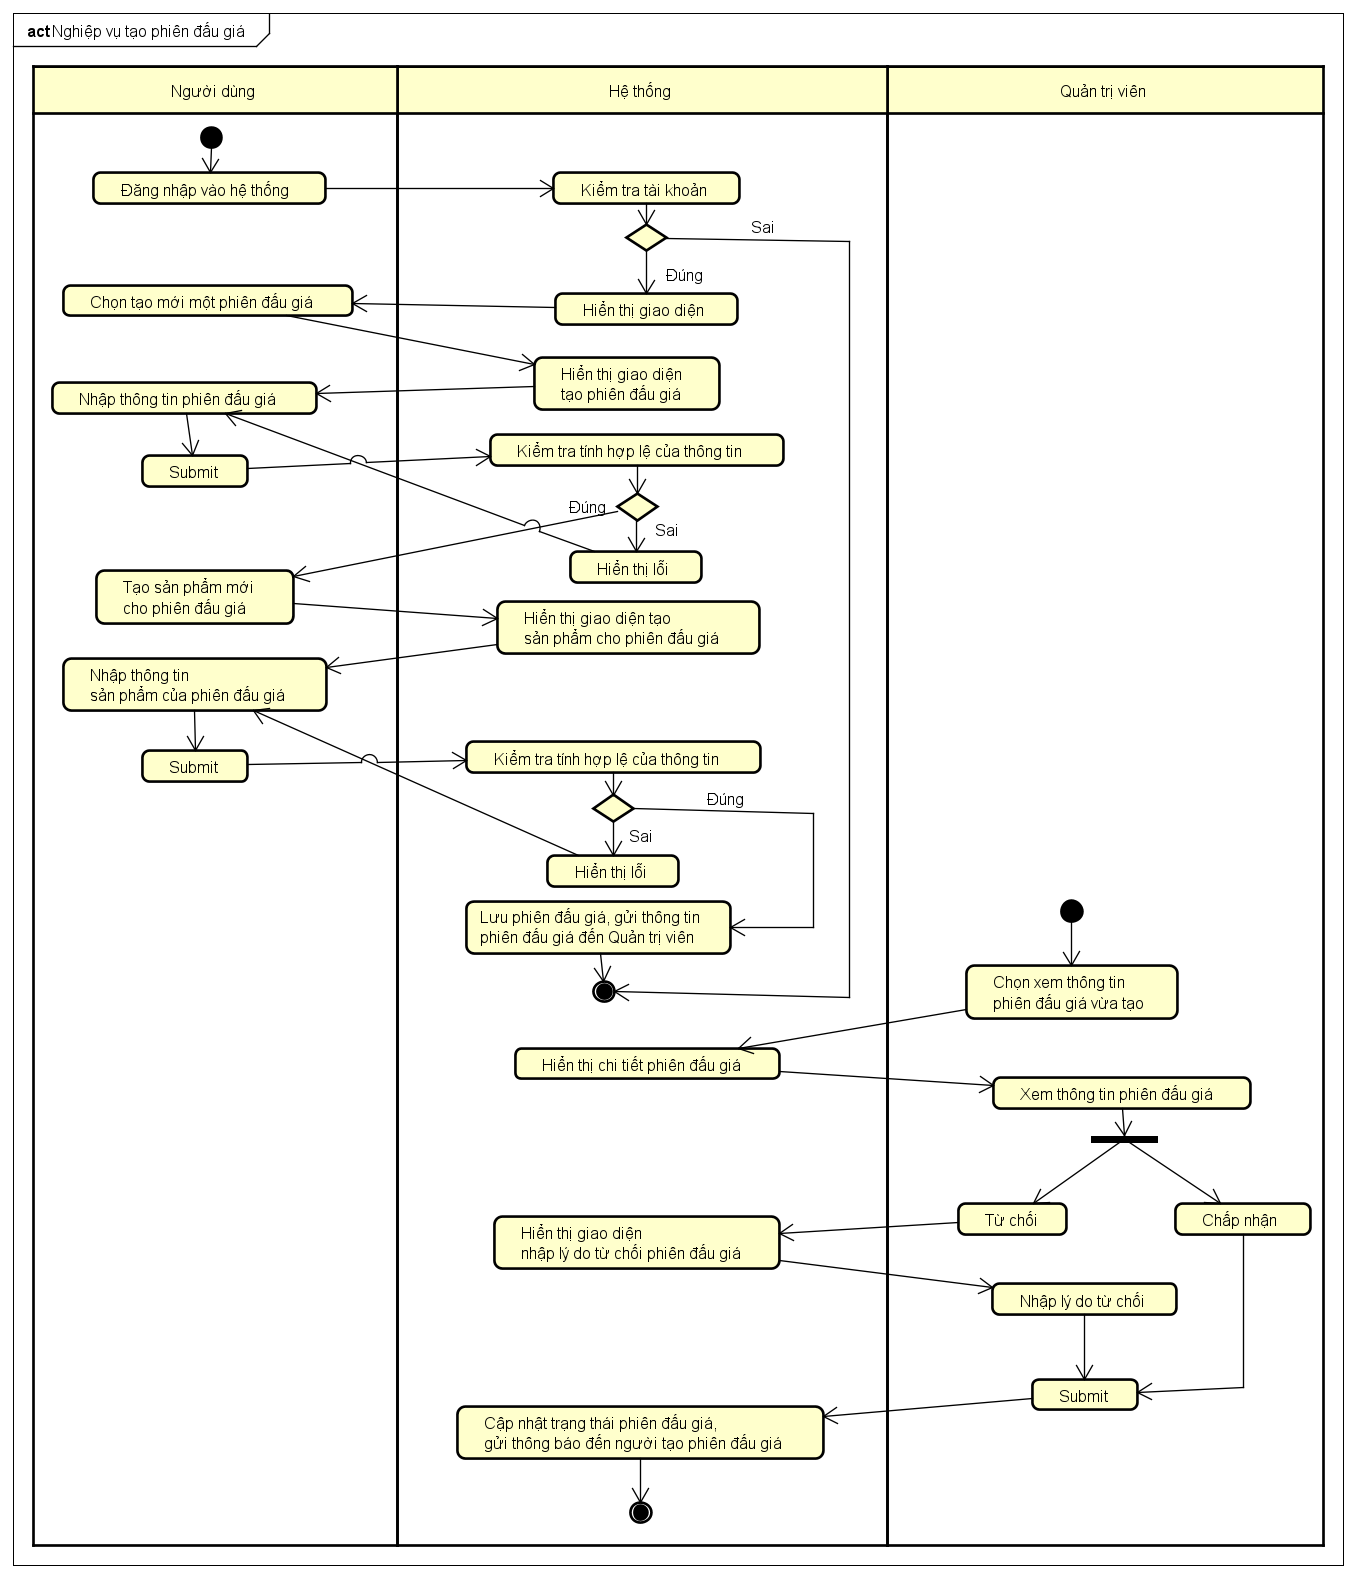
\includegraphics[width=11.4cm,height=13.28cm]{images/nghiệp vụ tạo phiên đấu giá.png}
    \caption{Nghiệp vụ tạo phiên đấu giá}
    \label{hinh27}
\end{figure}
Hình \ref{hinh27} mô tả nghiệp vụ tạo một phiên đấu giá. Người dùng đăng nhập vào hệ thống, chọn mục Bán hàng để tạo mới một phiên đấu giá. Người dùng nhập các thông tin theo form tạo mới phiên đấu giá, nếu thông tin không hợp lệ thì hệ thống sẽ báo lỗi ngay dưới trường đó. Sau khi tạo phiên đấu giá thành công thì hệ thống sẽ chuyển qua giao diện tạo mới sản phẩm cho phiên đấu giá đó. Tương tự người dùng cần nhập thông tin đầy đủ và hợp lệ, nếu không thì hệ thống sẽ báo lỗi ngay dưới trường không hợp lệ. Sau khi tạo mới sản phẩm xong thì người dùng phải đợi phía Admin phê duyệt. Phía Admin có nhiệm vụ chấp nhận hay từ chối phiên đấu giá, sau đó hệ thống sẽ cập nhật lại trạng thái phiên đấu giá.
\paragraph{Nghiệp vụ tạo phiên đấu giá}\mbox{}
\begin{figure}[H]
    \centering
    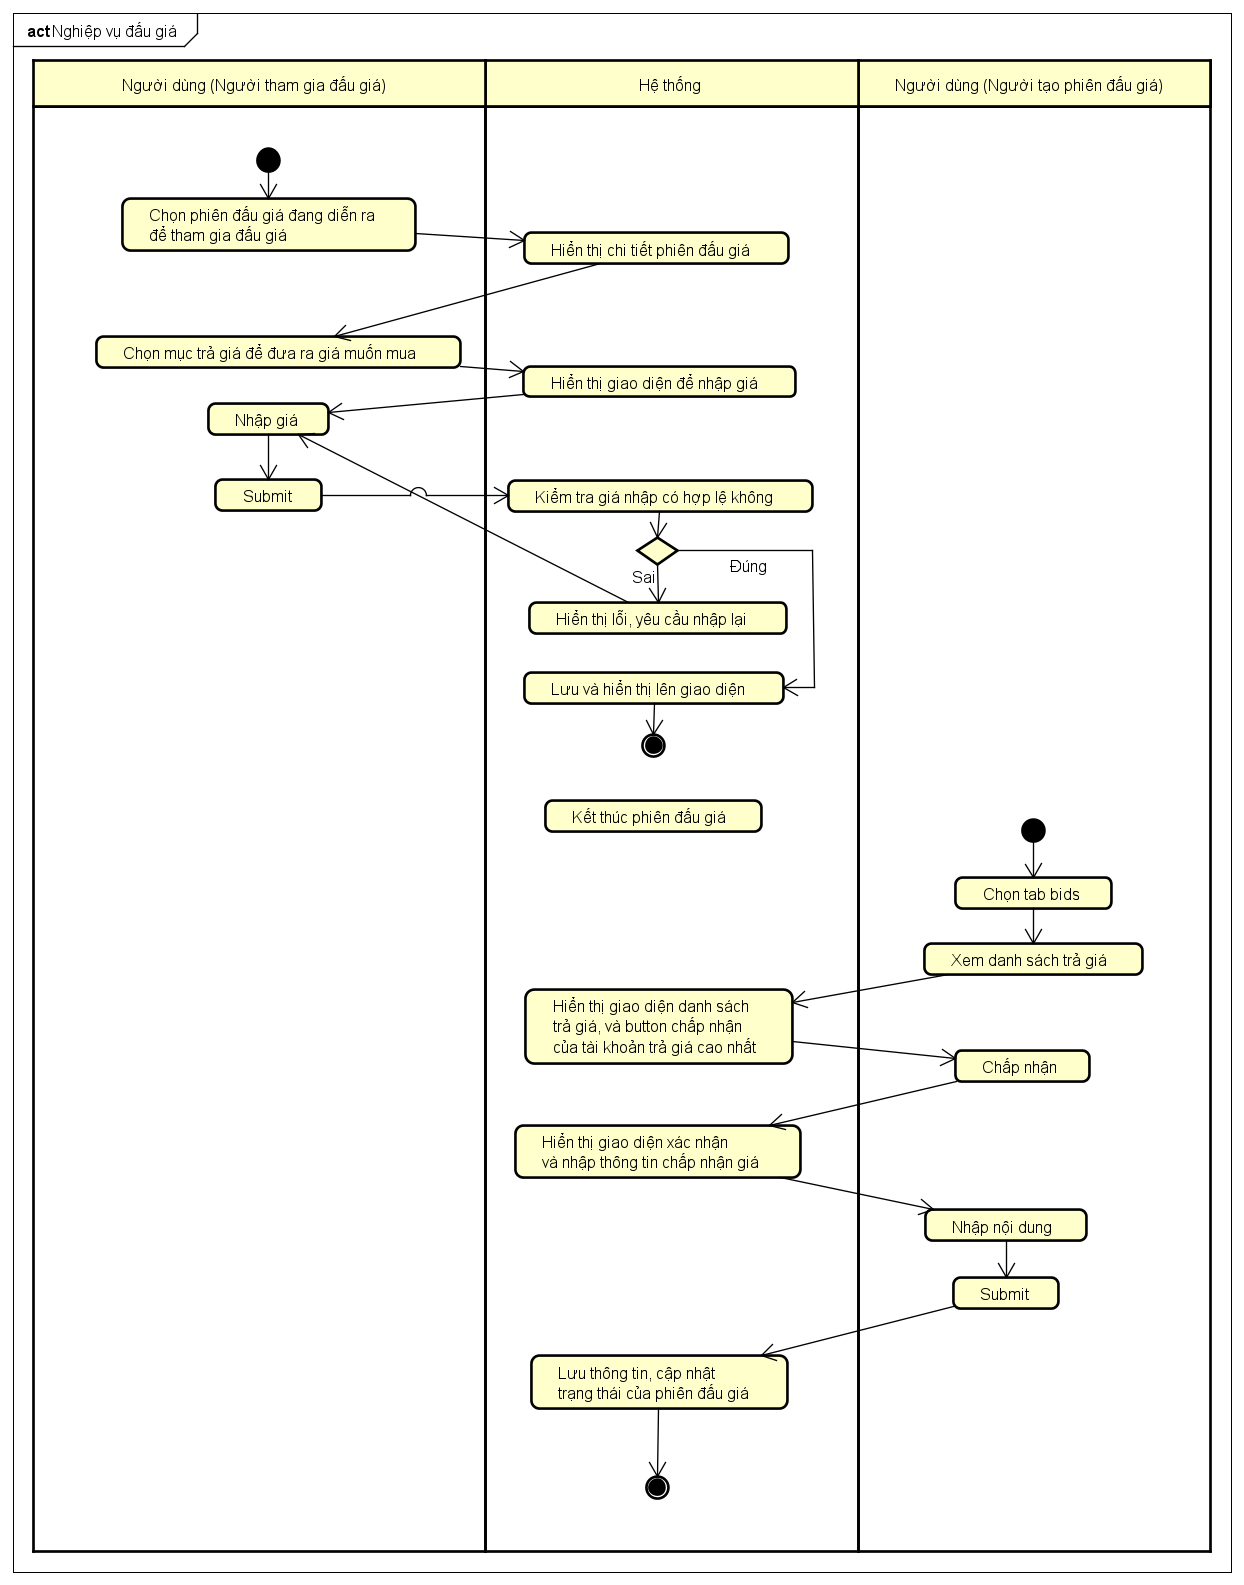
\includegraphics[width=11.4cm,height=14.54cm]{images/nghiệp vụ đấu giá.png}
    \caption{Nghiệp vụ tạo phiên đấu giá}
    \label{hinh28}
\end{figure}
Hình \ref{hinh28} mô tả nghiệp vụ Đấu giá. Khi một phiên đấu giá đang diễn ra thì Người dùng có thể tham gia trả giá. Người dùng chọn mục trả giá, nhập giá hợp lệ. Nếu giá mà người dùng đưa ra không lớn hơn trả giá cao nhất hiện tại hay không phải là số thì hệ thống sẽ báo lỗi dưới ô nhập giá. Khi phiên đấu giá kết thúc thì tại tài khoản của Người tạo phiên đấu giá đó sẽ hiển thị nút Chấp nhận với lượt trả giá cao nhất. Sau khi Người tạo phiên đấu giá xác nhận thì Hệ thống cập nhật trạng thái phiên đấu giá.
\subsection{Đặc tả chức năng}
\subsubsection{Đặc tả use case Tạo phiên đấu giá}
%\begin{table}[H]
    %\centering
    \begin{longtable}{| p{.25\textwidth} | p{.15\textwidth} | p{.15\textwidth} | p{.30\textwidth} |} 
    \caption{Đặc tả usecase Tạo phiên đấu giá}
    \label{bang22}
    \endfirsthead
    \endhead
    \hline
        \bfseries Mã Use case & \bfseries UC0001 & \bfseries Tên Use case & \bfseries Tạo phiên đấu giá \\\hline
        \bfseries Tác nhân hệ thống & \multicolumn{3}{c|}{Người dùng} \\\hline
        \bfseries Tiền điều kiện & \multicolumn{3}{c|}{Đăng nhập} \\\hline
        \bfseries Luồng sự kiện chính & \multicolumn{3}{c|}{
        \begin{tabular}{| p{.05\textwidth} | p{.15\textwidth} | p{.40\textwidth} |} 
            \hline
                \bfseries STT & \bfseries Thực hiện &  \bfseries Hành động \\\hline
                1 & Người dùng & Chọn chức năng tạo mới phiên đấu giá \\\hline
                2 & Hệ thống & Hiển thị giao diện tạo phiên đấu giá \\\hline
                3 & Người dùng & Nhập thông tin phiên đấu giá. Nhấn xác nhận \\\hline
                4 & Hệ thống & Kiểm tra tính hợp lệ của các trường thông tin mà Người dùng đã nhập \\\hline
                5 & Hệ thống & Lưu trữ thông tin phiên đấu giá vào cơ sở dữ liệu. Chuyển hướng qua trang tạo sản phẩm cho phiên đấu giá \\\hline
                6 & Hệ thống & Hiển thị thông tin của phiên đấu giá vừa tạo và giao diện để tạo sản phẩm cho phiên đấu giá \\\hline
                7 & Người dùng & Nhập thông tin sản phẩm cho phiên đấu giá tương ứng và xác nhận \\\hline
                8 & Hệ thống & Kiểm tra tính hợp lệ của các trường thông tin.  \\\hline
                9 & Hệ thống & Lưu thông tin sản phẩm vào cơ sở dữ liệu. Chuyển hướng đến trang cá nhân của người dùng đang đăng nhập \\\hline
        \end{tabular}
        }\\\hline
        \bfseries Luồng sự thay thế & \multicolumn{3}{c|}{
        \begin{tabular}{| p{.05\textwidth} | p{.15\textwidth} | p{.40\textwidth} |} 
            \hline
                \bfseries STT & \bfseries Thực hiện &  \bfseries Hành động \\\hline
                4a & Hệ thống & Thông báo các trường yêu cầu phải nhập, hoặc các giá trị nhập không hợp lệ \\\hline
                8a & Hệ thống & Thông báo các trường yêu cầu phải nhập, hoặc các giá trị nhập không hợp lệ \\\hline
        \end{tabular}
        }\\\hline
        \bfseries Hậu điều kiện & \multicolumn{3}{c|}{Không}\\\hline
    \end{longtable}
%\end{table}
\subsubsection{Đặc tả use case Từ chối phiên đấu giá}
%\begin{table}[H]
    %\centering
    \begin{longtable}{| p{.25\textwidth} | p{.15\textwidth} | p{.15\textwidth} | p{.30\textwidth} |} 
    \caption{Đặc tả usecase Từ chối phiên đấu giá}
    \label{bang23}
    \endfirsthead
    \endhead
    \hline
        \bfseries Mã Use case & \bfseries UC0002 & \bfseries Tên Use case & \bfseries Từ chối phiên đấu giá \\\hline
        \bfseries Tác nhân hệ thống & \multicolumn{3}{c|}{Quản trị viên} \\\hline
        \bfseries Tiền điều kiện & \multicolumn{3}{c|}{Đăng nhập với vai trò là quản trị viên} \\\hline
        \bfseries Luồng sự kiện chính & \multicolumn{3}{c|}{
        \begin{tabular}{| p{.05\textwidth} | p{.15\textwidth} | p{.40\textwidth} |} 
            \hline
                \bfseries STT & \bfseries Thực hiện &  \bfseries Hành động \\\hline
                1 & Quản trị viên & Chọn danh sách phiên đấu giá đang chờ duyệt \\\hline
                2 & Quản trị viên & Chọn vào phiên đấu giá muốn phê duyệt \\\hline
                3 & Hệ thống & Hiển thị thông tin chi tiết của phiên đấu giá đó \\\hline
                4 & Quản trị viên & Chọn từ chối \\\hline
                5 & Hệ thống & Lưu trữ thông tin phiên đấu giá vào cơ sở dữ liệu. Chuyển hướng qua trang tạo sản phẩm cho phiên đấu giá \\\hline
                6 & Quản trị viên & Nhập lý do từ chối, xác nhận \\\hline
                7 & Hệ thống & Kiểm tra tính hợp lệ của thông tin\\\hline
                8 & Hệ thống & Lưu lý do từ chối phiên đấu giá và gửi thông báo đến Người dùng. Cập nhật trạng thái của phiên đấu giá  \\\hline
                9 & Hệ thống & Chuyển hướng về danh sách phiên đấu giá chờ duyệt \\\hline
        \end{tabular}
        }\\\hline
        \bfseries Luồng sự thay thế & \multicolumn{3}{c|}{
        \begin{tabular}{| p{.05\textwidth} | p{.15\textwidth} | p{.40\textwidth} |} 
            \hline
                \bfseries STT & \bfseries Thực hiện &  \bfseries Hành động \\\hline
                7a & Hệ thống & Thông báo cần nhập lý do từ chối nếu Quản trị viên không nhập lý do mà xác nhận luôn. \\\hline
        \end{tabular}
        }\\\hline
        \bfseries Hậu điều kiện & \multicolumn{3}{c|}{Không}\\\hline
    \end{longtable}
%\end{table}
\subsubsection{Đặc tả use case Chấp nhận giá}
%\begin{table}[H]
    %\centering
    \begin{longtable}{| p{.25\textwidth} | p{.15\textwidth} | p{.15\textwidth} | p{.30\textwidth} |} 
    \caption{Đặc tả usecase Chấp nhận giá}
    \label{bang24}
    \endfirsthead
    \endhead
    \hline
        \bfseries Mã Use case & \bfseries UC0002 & \bfseries Tên Use case & \bfseries Chấp nhận giá \\\hline
        \bfseries Tác nhân hệ thống & \multicolumn{3}{c|}{Người dùng} \\\hline
        \bfseries Tiền điều kiện & \multicolumn{3}{c|}{Đăng nhập} \\\hline
        \bfseries Luồng sự kiện chính & \multicolumn{3}{c|}{
        \begin{tabular}{| p{.05\textwidth} | p{.15\textwidth} | p{.40\textwidth} |} 
            \hline
                \bfseries STT & \bfseries Thực hiện &  \bfseries Hành động \\\hline
                1 & Người dùng & Chọn chấp nhận\\\hline
                2 & Hệ thống & Hiển thị giao diện nhập thông tin thêm về việc chấp nhận giá \\\hline
                3 & Người dùng & Nhập thông tin, Xác nhận\\\hline
                4 & Hệ thống & Kiểm tra tính hợp lệ của thông tin \\\hline
                5 & Hệ thống & Lưu thông tin vào cơ sở dữ liệu, cập nhật trạng thái của phiên đấu giá\\\hline
                6 & Hệ thống & Chuyển hướng đến trang cá nhân của người dùng đang đăng nhập \\\hline
        \end{tabular}
        }\\\hline
        \bfseries Luồng sự thay thế & \multicolumn{3}{c|}{
        \begin{tabular}{| p{.05\textwidth} | p{.15\textwidth} | p{.40\textwidth} |} 
            \hline
                \bfseries STT & \bfseries Thực hiện &  \bfseries Hành động \\\hline
                4a & Hệ thống & Thông báo yêu cầu nhập khi người dùng không nhập thông tin về việc chấp nhận giá mà xác nhận luôn. \\\hline
        \end{tabular}
        }\\\hline
        \bfseries Hậu điều kiện & \multicolumn{3}{c|}{Không}\\\hline
    \end{longtable}
%\end{table}
\subsubsection{Đặc tả use case Tìm kiếm thông tin}
%\begin{table}[H]
    %\centering
    \begin{longtable}{| p{.25\textwidth} | p{.15\textwidth} | p{.15\textwidth} | p{.30\textwidth} |} 
    \caption{Đặc tả usecase Tìm kiếm thông tin}
    \label{bang25}
    \endfirsthead
    \endhead
    \hline
        \bfseries Mã Use case & \bfseries UC0002 & \bfseries Tên Use case & \bfseries Tìm kiếm thông tin \\\hline
        \bfseries Tác nhân hệ thống & \multicolumn{3}{c|}{Khách} \\\hline
        \bfseries Tiền điều kiện & \multicolumn{3}{c|}{Không} \\\hline
        \bfseries Luồng sự kiện chính & \multicolumn{3}{c|}{
        \begin{tabular}{| p{.05\textwidth} | p{.15\textwidth} | p{.40\textwidth} |} 
            \hline
                \bfseries STT & \bfseries Thực hiện &  \bfseries Hành động \\\hline
                1 & Khách & Chọn loại Tìm kiếm thông tin \\\hline
                2 & Khách & Nhập từ khóa tìm kiếm, nhấn vào icon tìm kiếm \\\hline
                3 & Hệ thống & Tìm kiếm trong hệ thống theo từ khóa và nhóm tìm kiếm mà Khách đã chọn. \\\hline
                4 & Hệ thống & Hiển thị các kết quả tìm kiếm \\\hline
        \end{tabular}
        }\\\hline
        \bfseries Luồng sự thay thế & \multicolumn{3}{c|}{
        \begin{tabular}{| p{.05\textwidth} | p{.15\textwidth} | p{.40\textwidth} |} 
            \hline
                \bfseries STT & \bfseries Thực hiện &  \bfseries Hành động \\\hline
                4a & Hệ thống & Nếu không tìm thấy kết quả nào thì hệ thống không hiển thị thông tin gì.\\\hline
        \end{tabular}
        }\\\hline
        \bfseries Hậu điều kiện & \multicolumn{3}{c|}{Không}\\\hline
    \end{longtable}
%\end{table}
\subsubsection{Đặc tả use case Đánh giá}
%\begin{table}[H]
    %\centering
    \begin{longtable}{| p{.25\textwidth} | p{.15\textwidth} | p{.15\textwidth} | p{.30\textwidth} |} 
    \caption{Đặc tả usecase Đánh giá}
    \label{bang26}
    \endfirsthead
    \endhead
    \hline
        \bfseries Mã Use case & \bfseries UC0002 & \bfseries Tên Use case & \bfseries Đánh giá \\\hline
        \bfseries Tác nhân hệ thống & \multicolumn{3}{c|}{Đánh giá} \\\hline
        \bfseries Tiền điều kiện & \multicolumn{3}{c|}{Đã đăng nhập, sau khi nhận được hàng} \\\hline
        \bfseries Luồng sự kiện chính & \multicolumn{3}{c|}{
        \begin{tabular}{| p{.05\textwidth} | p{.15\textwidth} | p{.40\textwidth} |} 
            \hline
                \bfseries STT & \bfseries Thực hiện &  \bfseries Hành động \\\hline
                1 & Khách & Chọn Đã nhận được hàng \\\hline
                2 & Hệ thống & Hiển thị form đánh giá sản phẩm của phiên đấu giá \\\hline
                3 & Khách & Nhập các thông tin, xác nhận \\\hline
                4 & Hệ thống & Kiểm tra tính hợp lệ của thông tin \\\hline
                5 & Hệ thống & Lưu thông tin đánh giá vào cơ sở dữ liệu. \\\hline
        \end{tabular}
        }\\\hline
        \bfseries Luồng sự thay thế & \multicolumn{3}{c|}{
        \begin{tabular}{| p{.05\textwidth} | p{.15\textwidth} | p{.40\textwidth} |} 
            \hline
                \bfseries STT & \bfseries Thực hiện &  \bfseries Hành động \\\hline
                4a & Hệ thống & Thông báo lỗi khi người dùng không nhập thông tin các trường cần thiết hay nhập sai định dạng. \\\hline
        \end{tabular}
        }\\\hline
        \bfseries Hậu điều kiện & \multicolumn{3}{c|}{Không}\\\hline
    \end{longtable}
%\end{table}
\subsection{Yêu cầu phi chức năng}
\subsubsection{Yêu cầu về kỹ thuật}
\begin{itemize}
    \item Website phân quyền người sử dụng: tùy theo từng nhóm người dùng sẽ có những quyền hạn truy cập, sử dụng những tính năng nhất định. 
    \item Mật khẩu của người dùng được mã hóa trước khi lưu vào cơ sở dữ liệu (mã hóa theo chuẩn Bcrypt).
    \item Sử dụng Single Page nên thời gian phản hồi giữa các màn hình nằm trong giới hạn cho phép.
    \item Phản hồi các thao tác của người dùng nhanh chóng.
    \item Hệ thống hoạt động ổn định, trong thời gian làm việc không gặp lỗi quá lớn.
    \item Hệ thống đảm bảo tính dễ bảo trì, dễ mở rộng trong tương lai
\end{itemize}
\subsubsection{Yêu cầu về giao diện người dùng}
\begin{itemize}
    \item Giao diện đẹp, đơn giản, dễ sử dụng, thân thiện với người dùng
    \item Hệ thống thông báo lỗi rõ ràng, chính xác trong các trường hợp người dùng nhập các trường thông tin không hợp lệ.
    \item Các nút, tiêu đề rõ ràng, dễ hiểu, có tính gợi nhớ
    \item Thực hiện phân trang để chia nhỏ những danh sách quá dài
\end{itemize}
\newpage

\section*{CHƯƠNG 3 CÔNG NGHỆ SỬ DỤNG}
\addcontentsline{toc}{section}{\numberline{}CHƯƠNG 3 CÔNG NGHỆ SỬ DỤNG}
\setcounter{section}{3}
\setcounter{subsection}{0}
\subsection{PHP Framework Laravel}
PHP viết tắt của cụm từ “PHP: Hypertext Preprocessor”, là ngôn ngữ lập trình mã nguồn mở phía server được thiết kế để xây dựng hệ thống web động.\\
PHP có thể chạy trên nhiều hệ điều hành phổ biến hiện nay như là Windows, Linux, Unix, Mac OS X…., tương thích với hầu hết các máy chủ được sử dụng ngày nay như Apache, IIS…Hiện nay PHP có khá nhiều Framework được xây dựng từ PHP nên quá trình tạo một website được rút gọn khá nhiều. \\
Laravel là một PHP Framework mã nguồn mở miễn phí, được phát triển bởi Taylor Otwell, nhằm mục đích hỗ trợ cho các ứng dụng web theo cấu trúc MVC. Laravel được hỗ trợ bởi một cộng đồng lớn nên quá trình phát triển dễ dàng hơn. \\
Một số đặc điểm quan trọng của Framework Laravel là: cung cấp mã CSRF để bảo toàn về bảo mật, có khuôn Blade hỗ trợ trong việc phát triển giao diện và cho phép sử dụng mã PHP trong blade.\\
Vì vậy trong đồ án Website đấu giá trực tuyến dùng ngôn ngữ PHP framework Laravel để xây dựng hệ thống quản lý bên admin và xây dựng restful api cho phía client. 
\subsection{ReactJs}
ReactJs là một thư viện JavaScript mã nguồn mở để xây dựng các thành phần giao diện người dùng có thể tái sử dụng. Trong mô hình MVC, ReactJs đóng vai trò như là View.\\
Một số đặc điểm quan trọng của ReactJs: Một ứng dụng React được xây dựng bởi nhiều Component khác nhau, mỗi Component sẽ chịu một trách nhiệm riêng, đảm bảo được tính tái sử dụng, dễ bảo trì. Khi sử dụng ReactJs thì có thể phát triển một Single Page Application, giúp nâng cao trải nghiệm người dùng. ReactJs được phát hành bởi FaceBook Inc, tài liệu phát hành theo giấy phép Creative Common 4.0.\\
ReactJs đơn giản và nhẹ, nó chỉ thao tác với lớp View trong mô hình MVC. ReactJs cũng có hiệu năng cao hơn và cũng không phức tạp bằng Angular hay Ember. ReactJs có hiệu năng tốt vì nó sử dụng DOM ảo, khi hệ thống tạo một Component mới, nó sẽ không thực sự ghi trực tiếp vào DOM trên trình duyệt mà ghi vào một DOM ảo, sau đó React sẽ sử dụng DOM ảo đó tạo ra DOM cho trình duyệt, đảm bảo được thời gian đọc/ghi là tối thiểu. Nên hiệu năng của ứng dụng được cải thiện đáng kể. \\
Thêm vào đó ReactJs có bộ công cụ dành cho dev được cài đặt dưới dạng tiện ích mở rộng của Chrome là React Developer Tools và Redux Developer. Các công cụ này hỗ trợ cho việc theo dõi hành động gửi đi, sự thay đổi của giao diện, việc kiểm tra lỗi hay bảo trì ứng dụng được dễ dàng hơn.
\subsection{Bootstrap}
Bootstrap là một framework HTML, CSS và Javascript cho phép người dùng thiết kế một website theo chuẩn nhất định, là một trong những framework được sử dụng nhiều khi xây dựng website. Bootstrap dễ sử dụng, vì nó dựa trên HTML, CSS và Javascript. Bootstrap sử dụng Grid System nên mặc định hỗ trợ Responsive, vì được viết theo xu hướng Mobile First nên ưu tiên cho việc tương thích với giao diện trên thiết bị di động.\\
Ngoài ra thì Bootstrap cũng tương thích với hầu hết trình duyệt hiện nay như Chrome, Firefox, Internet Explorer, Safari, Opera…
\subsection{MySQL}
MySQL là một hệ thống quản trị cơ sở dữ liệu mã nguồn mở hoạt động theo mô hình client-server. MySQL quản lý dữ liệu thông qua các cơ sở dữ liệu, mỗi cơ sở dữ liệu có thể có nhiều bảng có quan hệ với nhau. MySQL là hệ quản trị cơ sở dữ liệu rất được ưa chuộng trên toàn thế giới, có rất nhiều tổ chức lớn đang sử dụng như Facebook, Twitter, Booking.com và Verizon. \\
MySQL được biết đến là hệ quản trị cơ sở dữ liệu có tốc độ cao, ổn định, dễ sử dụng và hoạt động trên nhiều hệ điều hành, có độ bảo mật cao. Ngoài ra MySQL hỗ trợ rất nhiều chức năng truy vấn, có khả năng mở rộng mạnh mẽ và được thực hiện nhanh chóng.\\
Trong hệ thống website đấu giá trực tuyến, đồ án sử dụng MySQL để quản lý cơ sở dữ liệu, các bảng cơ sở dữ liệu được sinh ra bằng việc chạy lệnh php artisan migrate tại source code auction-admin. MySQL là lựa chọn phù hợp để quản lý cơ sở dữ liệu kết hợp với PHP để xây dựng hệ thống website đấu giá trực tuyến.
\subsection{Socket.IO}
Socket.IO là thư viện cho phép giao tiếp độ trễ thấp, hai chiều và dựa trên các sự kiện giữa client-server. Socket.IO được xây dựng dựa trên giao thức WebSocket và cung cấp các bảo đảm bổ sung dự phòng cho HTTP long-polling hoặc tự động kết nối lại.\\ 
Thư viện Socket.IO giữ một kết nối TCP mở với máy chủ, có thể dẫn đến việc tiêu hao nhiều pin cho người dùng. Socket.IO không được sử dụng trong dịch vụ nền cho các ứng dụng di động. \\
Socket.IO giúp các bên ở những địa chỉ khác nhau có thể kết nối được với nhau và việc truyền dữ liệu ngay lập tức thông qua server trung gian. Được sử dụng nhiều trong ứng dụng realtime như chat, game online…\\
Trong website đấu giá trực tuyến đồ án đã sử dụng thư viện Socket.IO trong ứng dụng chat realtime.
\newpage

\section*{CHƯƠNG 4 PHÁT TRIỂN VÀ TRIỂN KHAI ỨNG DỤNG}
\addcontentsline{toc}{section}{\numberline{}CHƯƠNG 4 PHÁT TRIỂN VÀ TRIỂN KHAI ỨNG DỤNG}
\setcounter{section}{4}
\setcounter{subsection}{0}
\setcounter{figure}{0}
\setcounter{table}{0}
\subsection{Thiết kế kiến trúc}
\subsubsection{Mô hình kiến trúc MVC}
Website đấu giá trực tuyến được xây dựng dựa theo mô hình MVC. Sau đây em xin trình bày tổng quát về mô hình MVC thông qua hình vẽ bên dưới: 
\begin{figure}[H]
    \centering
    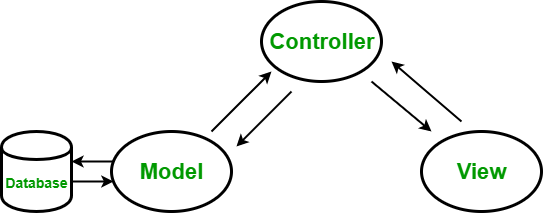
\includegraphics[width=10.6cm,height=4.15cm]{images/mvc.png}
    \caption{Mô hình kiến trúc MVC}
    \label{hinh41}
\end{figure}
Mô hình MVC là mẫu kiến trúc phân chia ứng dụng thành 3 thành phần chính: Model, View, Controller. Mỗi thành phần được xây dựng để xử lý các tác vụ khác nhau của một ứng dụng.
\begin{itemize}
    \item Lớp dữ liệu (Model) chịu trách nhiệm quản lý dữ liệu của ứng dụng, tương tác với hệ quản trị cơ sở dữ liệu. Lớp dữ liệu này không có bất kỳ liên quan logic nào đến việc hiển thị dữ liệu trên màn hình
    \item Lớp điều khiển ( Controller) đứng giữa lớp dữ liệu và lớp giao diện. Khi người dùng tương tác trên màn hình (View) thì phía lớp điều khiển sẽ nhận các yêu cầu đó, rồi gửi đến Model, sau khi Model xử lý logic xong, thì Controller nhận dữ liệu đó và trả ra màn hình View cho người dùng.
    \item Lớp giao diện (View) là nơi mà người dùng tương tác trực tiếp. Nhận yêu cầu đầu vào của người dùng rồi gửi đến lớp điều khiển (Controller), sau đó nhận lại dữ liệu từ lớp điều khiển và hiển thị ra màn hình người dùng.
\end{itemize}
Sau khi kết hợp giữa mô hình kiến trúc MVC và mô hình Client-Server thì website đấu giá trực tuyến sẽ có mô tả như hình dưới. 
\begin{figure}[H]
    \centering
    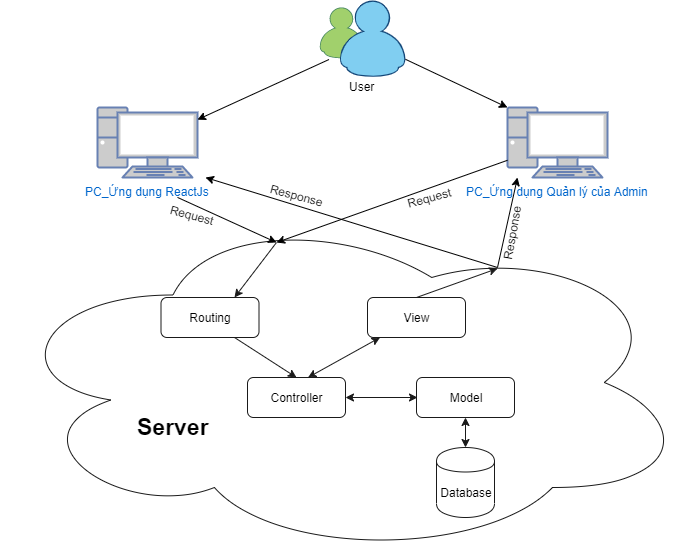
\includegraphics[width=11.4cm,height=9.22cm]{images/server.png}
    \caption{Mô hình hệ thống dựa theo kiến trúc MVC}
    \label{hinh42}
\end{figure}
Hệ thống được mô tả dựa trên kiến trúc MVC có thêm thành phần Routing có vai trò ánh xạ các request từ phía client đến controller.
\subsubsection{Thiết kế tổng quan}
Mô tả chi tiết các gói trong biểu đồ trên: 
Tầng giao diện cho ứng dụng web ( FontEndLayer)
\begin{figure}[H]
    \centering
    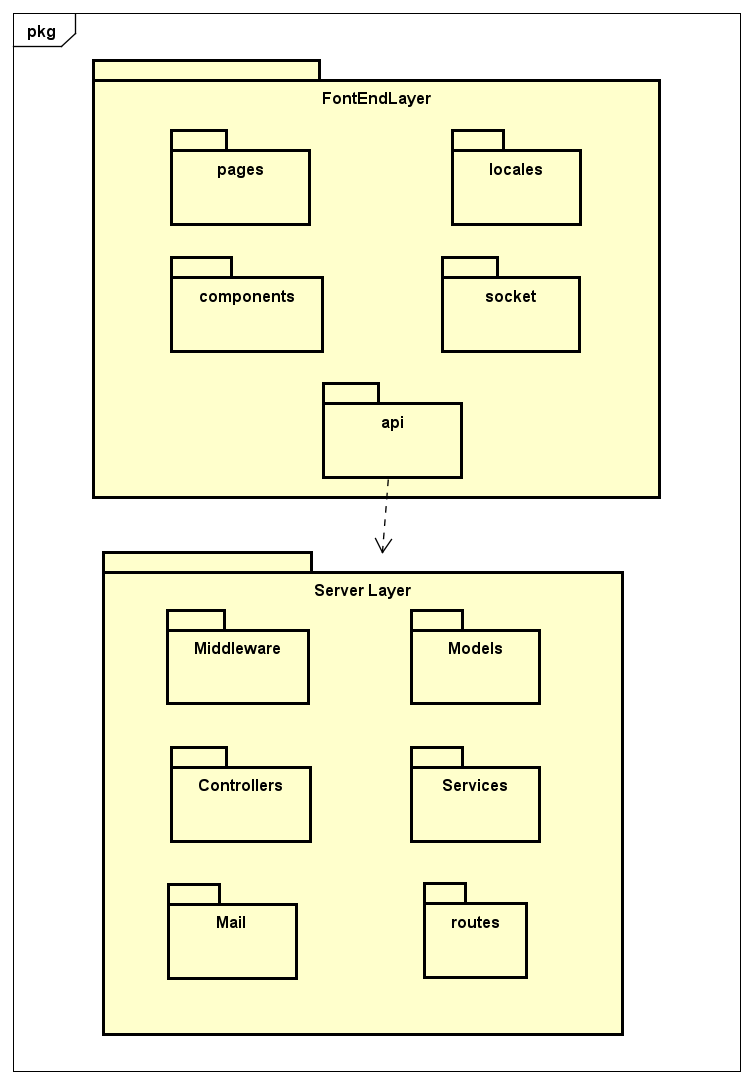
\includegraphics[width=11.4cm,height=12.92cm]{images/gói tổng quan.png}
    \caption{Biểu đồ gói tổng quan}
    \label{hinh43}
\end{figure}
\begin{itemize}
    \item pages: chứa các trang chính của website đấu giá trực tuyến
    \item components: chứa các component có thể tái sử dụng trên toàn website.
    \item locales: chứa các file phục vụ cho việc chuyển đổi ngôn ngữ giữa tiếng Nhật và tiếng Việt
    \item api: chứa các lời gọi restful api ở phía server
    \item socket: có nhiệm vụ trong việc quản lý tính realtime khi nhắn tin trực tuyến
\end{itemize}
Tầng ứng dụng server (Server Layer)
\begin{itemize}
    \item Middleware: Thành phần có nhiệm vụ đảm bảo người dùng hiện tại có đủ quyền để thực hiện tác vụ nào đó trước khi đưa đến Controllers xử lý.
    \item Controllers: Nhận các request từ phía người dùng. Controller có nhiệm vụ xử lý logic, giao tiếp với Model, nhận dữ liệu từ Model để trả response cho ứng dụng hiển thị lên màn hình.
    \item Models: Có nhiệm vụ định nghĩa cơ sở dữ liệu cho hệ thống, giao tiếp với cơ sở dữ liệu.
    \item Services: Có nhiệm vụ giao tiếp với cơ sở dữ liệu, nhằm giảm tải công việc cho Models
    \item Mail: Có nhiệm vụ trong việc gửi Mail, khi mà người dùng muốn liên lạc với Admin thông qua Mail
    \item routers: Có nhiệm vụ phân luồng cho các request gửi đến hệ thống
    \item view: hiển thị dữ liệu ra màn hình bên hệ thống admin
\end{itemize}
\subsubsection{Thiết kế chi tiết gói}
\paragraph{Thiết kế chi tiết gói cho ứng dụng web ( FontEndLayer)
} \mbox{}
\begin{figure}[H]
    \centering
    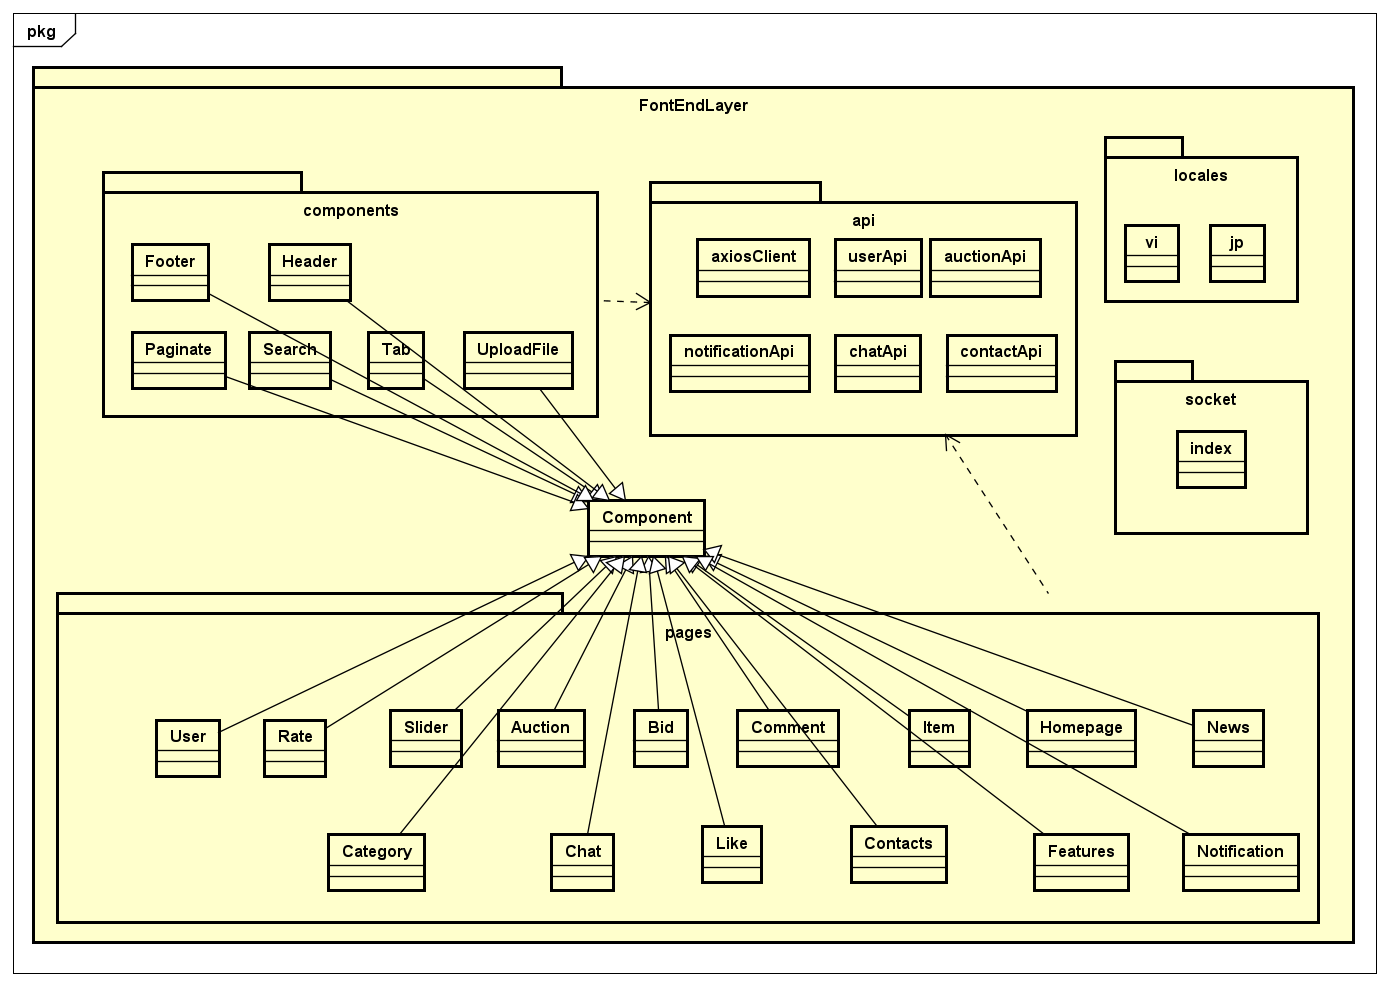
\includegraphics[width=11.4cm,height=6.34cm]{images/fontendlayer.png}
    \caption{Thiết kế chi tiết gói ứng dụng web}
    \label{hinh44}
\end{figure}
Trên ứng dụng web, tất cả các class sẽ được kết thừa từ Component của ReactJs.\\
Mỗi gói sẽ có một nhiệm vụ khác nhau: \\
Gói components sẽ chứa các thành phần có khả năng tái sử dụng trên toàn bộ website.
\begin{itemize}
    \item Footer: giao diện chân trang của tất cả các màn hình
    \item Header: giao diện thanh header hiển thị bên trên tất cả các màn hình
    \item Paginate: giao diện thanh phân trang ở tất cả các màn liệt kê danh sách
    \item Search: giao diện thanh tìm kiếm
    \item Tab: Giao diện thanh chia danh sách phiên đấu giá theo trạng thái
\end{itemize}
Gói pages chứa thành phần hiển thị trên màn hình client của website đấu giá trực tuyến
\begin{itemize}
    \item HomePage: giao diện trang chủ
    \item Features: danh sách phiên đấu giá tại trang chủ
    \item Slider: slide hiển thị tại trang chủ
    \item Category: danh sách loại sản phẩm tại trang chủ
    \item News: giao diện liên quan đến bản tin (danh sách, chi tiết bản tin)
    \item Contacts: giao diện khi liên lạc với Admin qua email
    \item Notifications: giao diện thông báo (danh sách, chi tiết thông báo)
    \item User: giao diện liên quan đến Người dùng ( đăng nhập, đăng ký, thay đổi mật khẩu, chỉnh sửa tài khoản)
    \item Auction: giao diện liên quan đến phiên đấu giá (thêm, sửa, danh sách, chi tiết phiên đấu giá)
    \item Item: giao diện liên quan đến sản phẩm của phiên đấu giá (thêm, sửa, chi tiết sản phẩm của phiên đấu giá) 
    \item Bid: giao diện liên quan đến trả giả (thêm, danh sách trả giá)
    \item Comment: giao diện liên quan đến bình luận ( thêm, xóa, danh sách bình luận)
    \item Rate: giao diện đánh giá sản phẩm khi nhận được hàng
    \item Chat: giao diện màn hình nhắn tin
    \item Like: giao diện thích một phiên đấu giá (yêu thích, danh sách yêu thích)
\end{itemize}
Gói api chứa các lời gọi restful api từ server.
\begin{itemize}
    \item axiosClient: định dạng chung lời gọi restful api
    \item userApi: lời gọi restful api liên quan đến người dùng
    \item auctionApi: lời gọi restful api liên quan đến phiên đấu giá
    \item notificationApi: lời gọi restful api liên quan đến thông báo
    \item chatApi: lời gọi restful api liên quan đến nhắn tin
    \item contactApi: lời gọi restful api liên quan đến liên lạc với Admin bằng email.
\end{itemize}
Gói locales chứa các file phục vụ cho việc chuyển đổi giữa tiếng Nhật và tiếng Việt.
\begin{itemize}
    \item jp: lưu trữ các key và text bằng tiếng Nhật tương ứng.
    \item vi: lưu trữ các key và text bằng tiếng Việt tương ứng.
\end{itemize}
Gói socket được gọi khi người dùng truy cập vào ứng dụng chat. Gói socket đảm bảo ứng dụng chat hoạt động realtime.
\paragraph{Thiết kế chi tiết gói cho server (ServerLayer)}
\begin{figure}[H]
    \centering
    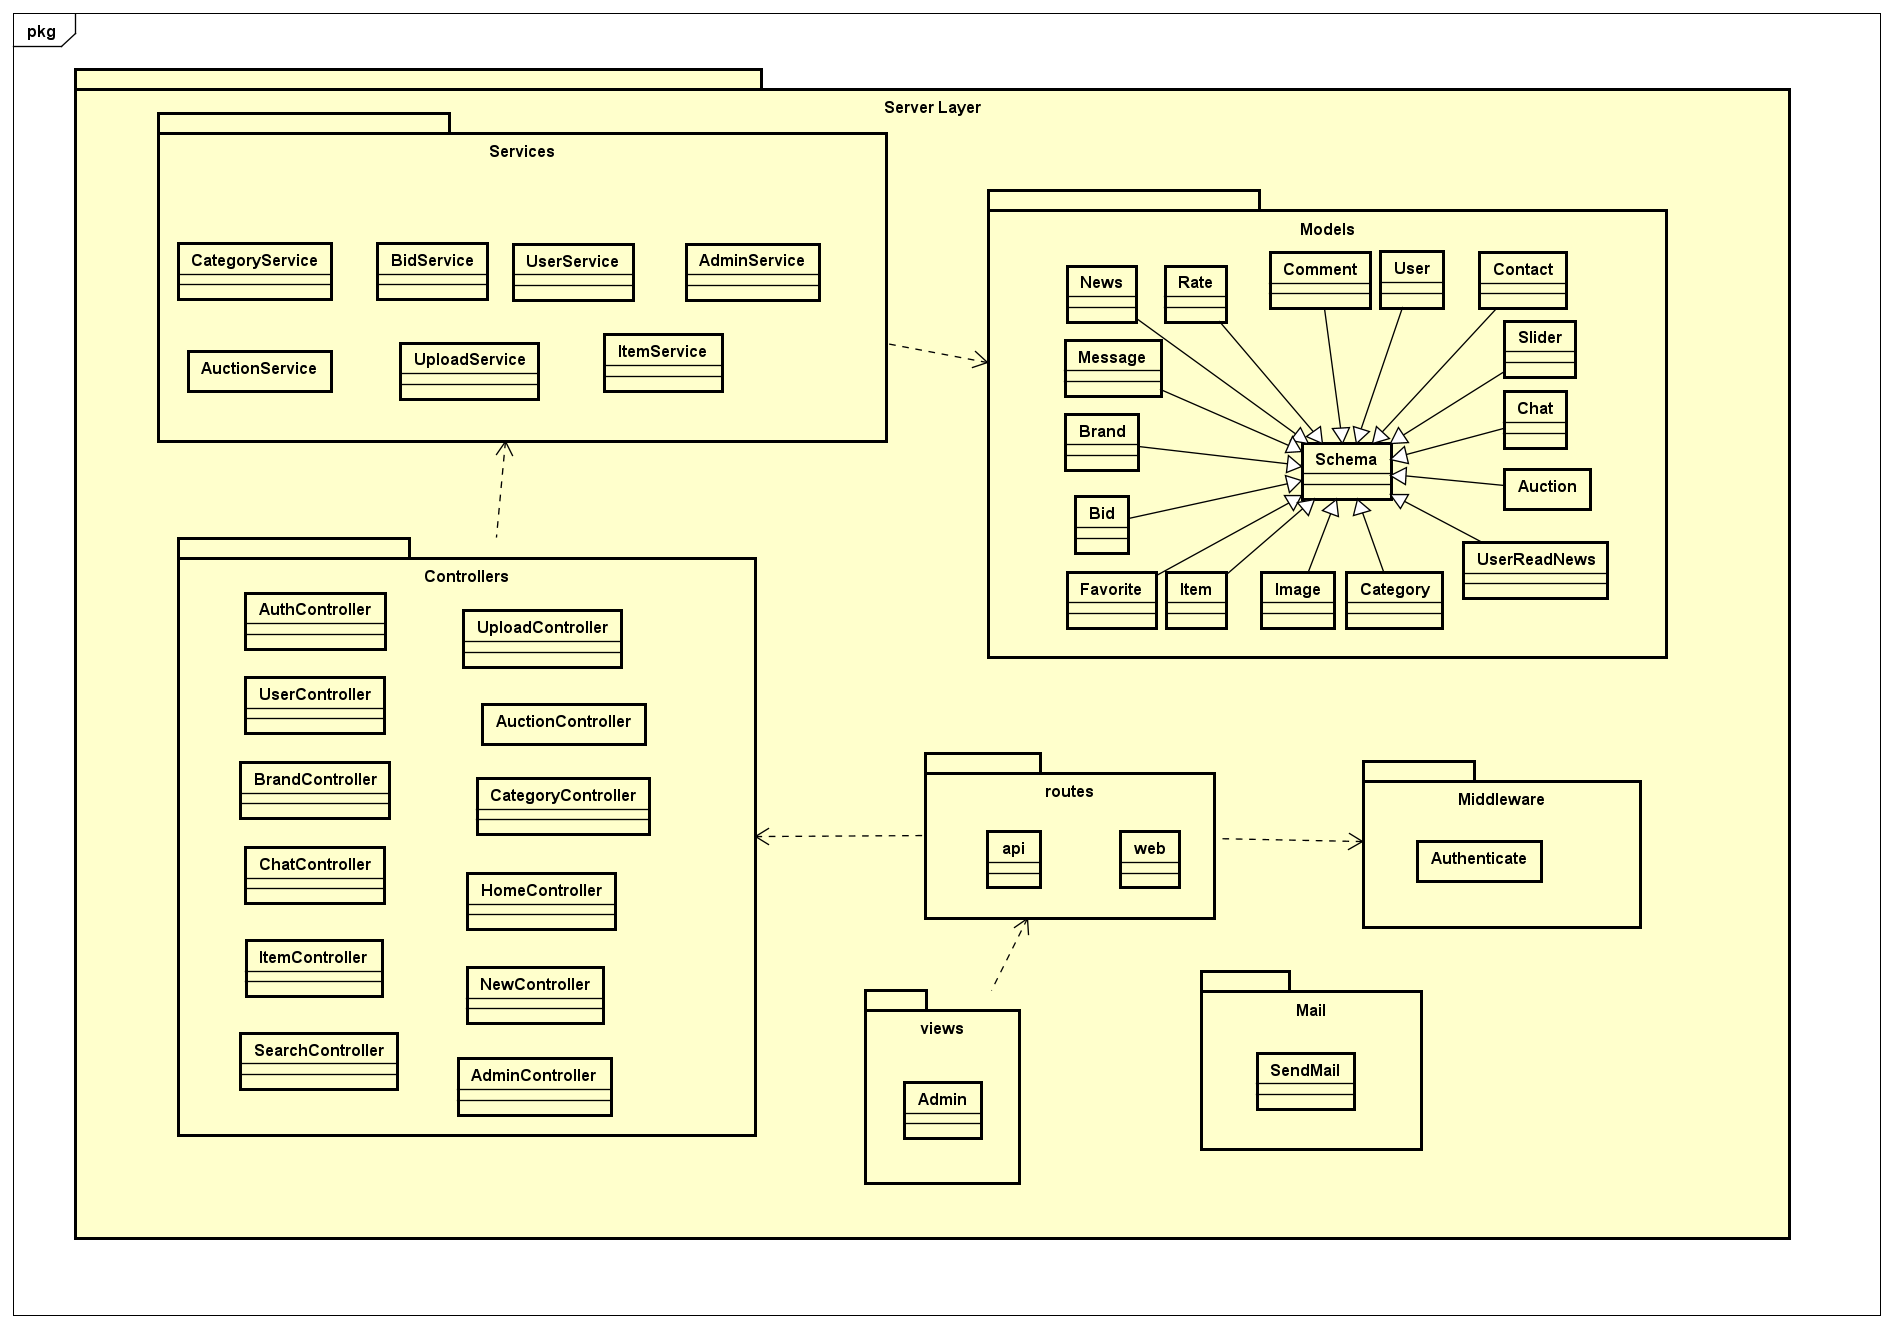
\includegraphics[width=11.4cm,height=8.0cm]{images/serverlayer.png}
    \caption{Thiết kế chi tiết gói serverlayer}
    \label{hinh45}
\end{figure}
Sau khi phía client gọi các restful api, hệ thống sẽ gửi request về cho controller phía trong gói Server Layer. Sau khi nhận được lời gọi thì phía controller sẽ gọi đến middleware để kiểm tra người dùng truy cập hay các tác vụ đó có đáp ứng điều kiện để thông qua được middleware không. Nếu thông qua middleware, thì dựa vào request được gửi tới, controller sẽ vào các model, service để lấy dữ liệu tương ứng rồi trả về cho client.\\ 
Sau đây là mô tả chi tiết các class có trong ServerLayer:\\
Gói routes có nhiệm vụ xử lý phân luồng cho các request gửi đến hệ thống
\begin{itemize}
    \item api: chứa các đường dẫn api xử lý phía client
    \item web: chứa các đường dẫn xử lý phía admin
\end{itemize}
Gói controllers:
\begin{itemize}
    \item AuthController: Xử lý các API liên quan đến việc xác minh tài khoản người dùng
    \item UserController: Xử lý các API liên quan đến tài khoản người dùng 
    \item AuctionController: Xử lý các API liên quan đến phiên đấu giá
    \item ItemController: Xử lý các API liên quan đến sản phẩm
    \item BrandController: Xử lý các API liên quan đến thương hiệu
    \item CategoryController: Xử lý các API liên quan đến loại sản phẩm
    \item ChatController: Xử lý các API liên quan đến nhắn tin
    \item NewController: Xử lý các API liên quan đến tin tức
    \item UploadController: Xử lý các API liên quan đến upload hình ảnh
    \item SearchController: Xử lý các API liên quan đến tìm kiếm
    \item HomeController: Xử lý các API liên quan đến trang chủ (slide)
    \item AdminController: Xử lý các sự kiện phía quản trị viên
\end{itemize}
Gói models
\begin{itemize}
    \item User: định nghĩa dữ liệu cho bảng users và quan hệ với các bảng khác trong cơ sở dữ liệu
    \item Auction: định nghĩa dữ liệu cho bảng auctions và quan hệ với các bảng khác trong cơ sở dữ liệu
    \item Item: định nghĩa dữ liệu cho bảng items và quan hệ với các bảng khác trong cơ sở dữ liệu
    \item Image: định nghĩa dữ liệu cho bảng images và quan hệ với các bảng khác trong cơ sở dữ liệu
    \item Category: định nghĩa dữ liệu cho bảng categories và quan hệ với các bảng khác trong cơ sở dữ liệu
    \item Brand: định nghĩa dữ liệu cho bảng brands và quan hệ với các bảng khác trong cơ sở dữ liệu
    \item Bid: định nghĩa dữ liệu cho bảng bids và quan hệ với các bảng khác trong cơ sở dữ liệu
    \item Comment: định nghĩa dữ liệu cho bảng comments và quan hệ với các bảng khác trong cơ sở dữ liệu
    \item News: định nghĩa dữ liệu cho bảng news và quan hệ với các bảng khác trong cơ sở dữ liệu
    \item UserReadNews: định nghĩa dữ liệu cho bảng userreadnews và quan hệ với các bảng khác trong cơ sở dữ liệu
    \item Contact: định nghĩa dữ liệu cho bảng contacts và quan hệ với các bảng khác trong cơ sở dữ liệu
    \item Slider: định nghĩa dữ liệu cho bảng sliders và quan hệ với các bảng khác trong cơ sở dữ liệu
    \item Favorites: định nghĩa dữ liệu cho bảng favorites và quan hệ với các bảng khác trong cơ sở dữ liệu
    \item Chat: định nghĩa dữ liệu cho bảng chat và quan hệ với các bảng khác trong cơ sở dữ liệu
    \item Message: định nghĩa dữ liệu cho bảng messages và quan hệ với các bảng khác trong cơ sở dữ liệu
    \item Rate: định nghĩa dữ liệu cho bảng rate và quan hệ với các bảng khác trong cơ sở dữ liệu
\end{itemize}
Gói services có nhiệm vụ giao tiếp với cơ sở dữ liệu (nhằm giảm tải công việc của Models)
\begin{itemize}
    \item UserService: xử lý các function thao tác với cơ sở dữ liệu liên quan đến người dùng
    \item AuctionService: xử lý các function thao tác với cơ sở dữ liệu liên quan đến phiên đấu giá
    \item ItemService: xử lý các function thao tác với cơ sở dữ liệu liên quan đến sản phẩm
    \item CategoryService: xử lý các function thao tác với cơ sở dữ liệu liên quan đến loại sản phẩm
    \item BidService: xử lý các function thao tác với cơ sở dữ liệu liên quan đến trả giá
    \item UploadService: xử lý các function thao tác với cơ sở dữ liệu liên quan đến upload hình ảnh
    \item AdminService: xử lý các function thao tác với cơ sở dữ liệu liên quan đến hệ thống quản trị viên
\end{itemize}
Gói views: 
\begin{itemize}
    \item Admin: gồm các trang quản lý dành cho quản trị viên
\end{itemize}
\subsection{Thiết kế chi tiết}
\subsubsection{Thiết kế giao diện}
Trong phần này em sẽ trình bày về các nguyên tắc chung khi thiết kế giao diện, và phác thảo một số màn hình chính, các thông số quan trọng của màn hình trong phần mềm đấu giá trực tuyến.
\paragraph{Thông số màn hình} \mbox{}
%\begin{table}[]
    %\centering
    \tablehead{%
    \hline
    \bfseries STT & \bfseries Thông tin & \bfseries Các thông số màn hình  \\\hline}
    \tabletail{\hline}
    \topcaption{Thông số màn hình trong thiết kế giao diện ứng dụng web của client}
    \label{bang41}
    \begin{supertabular}{| p{.15\textwidth} | p{.25\textwidth} | p{.50\textwidth} |} 
        1 & Kích thước màn hình &
            \begin{tabular}{p{.45\textwidth}}
                Máy tính bàn : \\
                (Desktops -Medium devices): >= 992px\\
                Máy tính lớn : \\
                (Large Desktops - Large devices) >= 1200px
            \end{tabular}\\\hline
        2 & Màu sắc &
            \begin{tabular}{p{.45\textwidth}}
                Màu nền: \#F8F9FA\\
                Màu tiêu đề: màu xanh \#7FAD39 hoặc màu đen \#000000\\
                Màu chữ thường: màu đen \#000000\\
                Màu liên kết: màu xanh nhạt \#E6EFE6, khi di chuyển chuột vào thì thành màu xanh đậm hơn một chút \#F8F9FA
            \end{tabular}\\\hline
        3 & Kiểu chữ &
        Segoe UI
        \\\hline
        4 & Ngôn ngữ &
        Tiếng Việt, Tiếng Nhật
        \\\hline
    \end{supertabular}\\
% \end{table}
\\
%\begin{table}[H]
    %\centering
     \tablehead{%
    \hline
    \bfseries STT & \bfseries Thông tin & \bfseries Các thông số màn hình  \\\hline}
    \tabletail{\hline}
    \topcaption{Thông số màn hình trong thiết kế giao diện ứng dụng web của hệ thống admin}
    \label{bang42}
    \begin{supertabular}{| p{.15\textwidth} | p{.25\textwidth} | p{.50\textwidth} |} 
    \hline
        1 & Kích thước màn hình &
            \begin{tabular}{p{.45\textwidth}}
                Máy tính bàn\\
                (Desktops -Medium devices): >= 992px\\
                Máy tính lớn\\
                (Large Desktops - Large devices)\\ 
                >= 1200px\\
                Di động: (Phones) <=768px\\
            \end{tabular}
        \\\hline
        2 & Màu sắc &
            \begin{tabular}{p{.45\textwidth}}
                Màu nền: xám trắng \#F8F9FA\\
                Màu tiêu đề: màu đen \#000000\\
                Màu chữ thường: màu đen \#000000 hoặc màu trắng \#fff\\
                Màu liên kết:  màu xanh nước biển \#007bff\\
            \end{tabular}
        \\\hline
        3 & Theme &
        AdminLTE
        \\\hline
        4 & Kiểu chữ &
        Segoe UI
        \\\hline
        5 & Ngôn ngữ &
        Tiếng Việt, Tiếng Nhật
        \\\hline
    \end{supertabular}
%\end{table}
\subsubsection{Nguyên tắc thiết kế chung}
Để website đáp ứng được yêu cầu dễ sử dụng, thân thiện với người dùng. Vì vậy đồ án phải đảm bảo khi người dùng nhìn vào sẽ biết chức năng của từng nút, nắm cơ bản luồng hoạt động của ứng dụng. Người dùng có thể dự đoán được nếu nhấn nút này hay bỏ qua trường này thì sẽ có điều gì xảy ra tiếp theo. Ví dụ ở các form đăng ký thì những trường bắt buộc sẽ được đánh dấu sao màu đỏ, thông báo đầy đủ lỗi khi người dùng nhập thông tin không phù hợp, các trường cần bảo mật thì ẩn thông tin khi nhập xong. Đặc biệt khi người dùng muốn xóa gì đó thì cần phải xác nhận lại thông tin, đảm bảo hành vi không phải là vô tình. Sau khi người dùng thực hiện xong các thao tác thì thông báo bằng các toast màu sắc phù hợp để dễ dàng nhận biết là tác vụ đã thành công hay chưa. \\
Ngoài ra để đảm bảo người dùng không cảm thấy khó chịu khi sử dụng website thì màu sắc của giao diện cũng cần được thống nhất, chọn tông màu sáng, nhẹ nhàng, không cho quá nhiều màu sắc sặc sỡ. Với các thông báo thì cần dùng màu sắc đặc trưng hay được dùng nhiều như tác vụ thành công màu \#28A475 (success), lỗi màu \#DC3545 (error), cảnh báo màu \#FFC107 (warning). Đối với các tác vụ mà có thể click chuột được thì khi di chuyển chuột vào sẽ phải thay đổi màu sắc để người dùng dễ nhận biết. Với các hộp thông báo thì hiển thị giữa màn hình, các thông tin bên dưới làm mờ để nổi bật hộp thông báo.
\subsubsection{Thiết kế sơ đồ hệ thống}
Sau đây đồ án sẽ trình bày sơ đồ màn hình của hệ thống phía Người dùng và hệ thống quản trị phía Quản trị viên.
\begin{figure}[H]
    \centering
    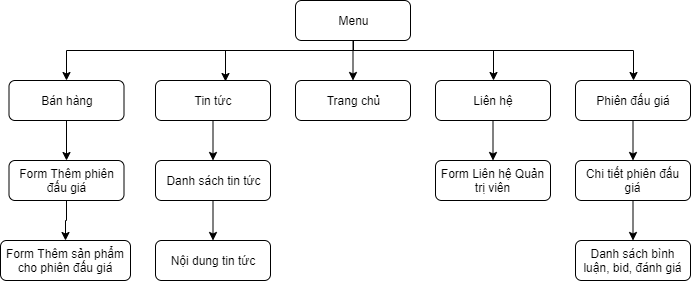
\includegraphics[width=11.4cm,height=4.65cm]{images/clientpage.png}
    \caption{Sơ đồ hệ thống phía Người dùng}
    \label{hinh46}
\end{figure}
Sơ đồ trên thể hiện phía giao diện Người dùng có 5 giao diện chính, i) Bán hàng: khi người dùng muốn tạo một phiên đấu giá thì sẽ thực hiện ở màn hình này, ii) Bài viết : Hiển thị những bài viết, tin tức mà phía Quản trị viên thêm vào, iii) Trang chủ:  Hiển thị danh sách các phiên đấu giá của toàn hệ thống, iv) Liên hệ: khi người dùng muốn liên hệ với Quản trị viên qua email. Cuối cùng là Phiên đấu giá bao gồm chi tiết phiên đấu giá và danh sách các bình luận, trả giá (bid), đánh giá của người dùng.
\begin{figure}[H]
    \centering
    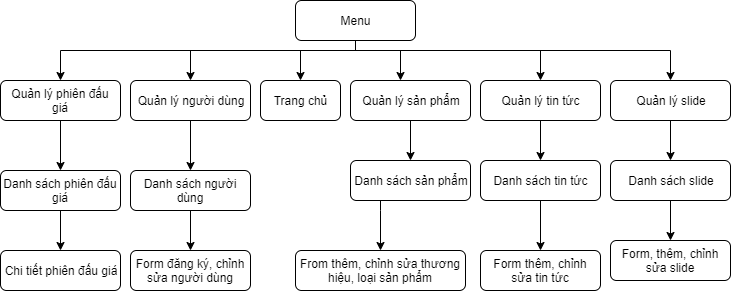
\includegraphics[width=11.4cm,height=4.54cm]{images/adminpage.png}
    \caption{Sơ đồ hệ thống phía Quản trị viên}
    \label{hinh47}
\end{figure}
Phía Quản trị viên có 6 giao diện chính trang chủ, quản lý phiên đấu giá, người dùng, sản phẩm, tin tức và slide
\subsubsection{Thiết kế phác thảo màn hình chính}
Sau đây là mockup một số màn hình chính i) giao diện trang chủ, ii) giao diện tạo phiên đấu giá, iii) giao diện thêm sản phẩm cho phiên đấu giá, iv) giao diện chi tiết phiên đấu giá
\begin{figure}[H]
    \centering
    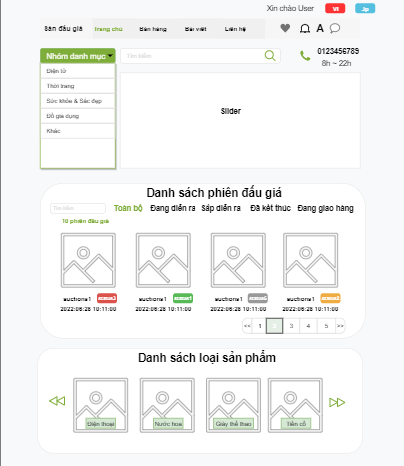
\includegraphics[width=7.87cm,height=9.07cm]{images/homepage.png}
    \caption{Mockup màn hình trang chủ}
    \label{hinh48}
\end{figure}
Hình \ref{hinh48} mô tả mockup giao diện màn hình trang chủ phía Người dùng. Phần header bao gồm tên tài khoản đang đăng nhập, icon chuyển đổi giữa tiếng Việt và Tiếng Nhật; tiếp theo là thanh navbar chứa tiêu đề của các page chính và icon liên quan (icon tim liên kết đến danh sách phiên đấu giá yêu thích, icon chuông liên kết đến danh sách thông báo, icon A liên kết đến trang cá nhân của người dùng, icon tin nhắn liên kết đến ứng dụng chat realtime). Tiếp đến website hiển thị nhóm danh mục loại sản phẩm, thanh tìm kiếm, slide hiển thị trên trang chủ, số điện thoại và thời gian mà admin có thể hỗ trợ. Trang chủ cũng hiển thị danh sách toàn bộ phiên đấu giá, loại sản phẩm hiện có trên toàn hệ thống. Phần footer chứa thông tin, địa chỉ, các tài khoản xã hội của website.
\begin{figure}[H]
    \centering
    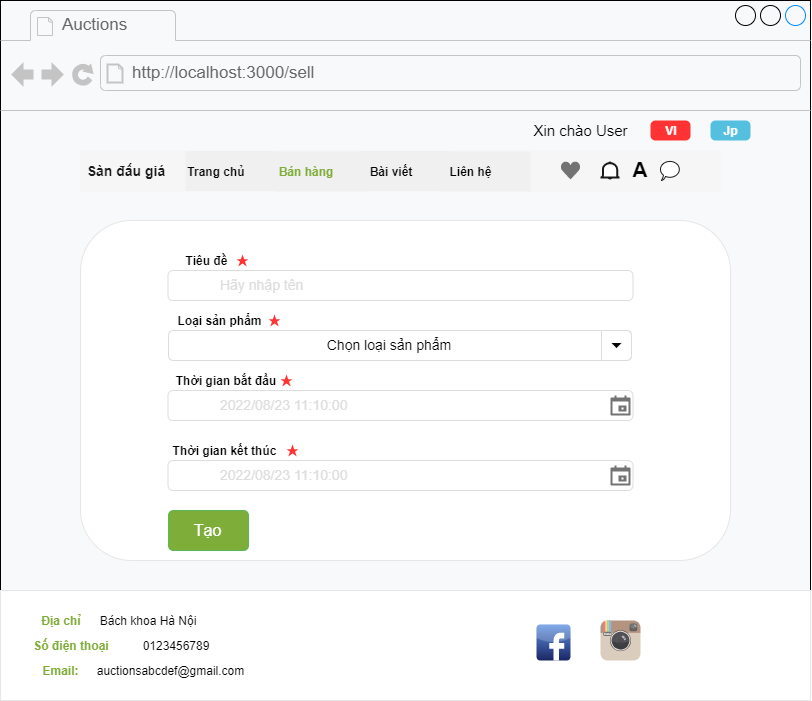
\includegraphics[width=11.43cm,height=9.87cm]{images/createauction.png}
    \caption{Mockup màn hình tạo phiên đấu giá}
    \label{hinh49}
\end{figure}
Hình \ref{hinh49} mô tả mockup giao diện tạo một phiên đấu giá. Những trường nào yêu cầu phải nhập sẽ có hình ngôi sao màu đỏ để người dùng dễ nhận biết.
\begin{figure}[H]
    \centering
    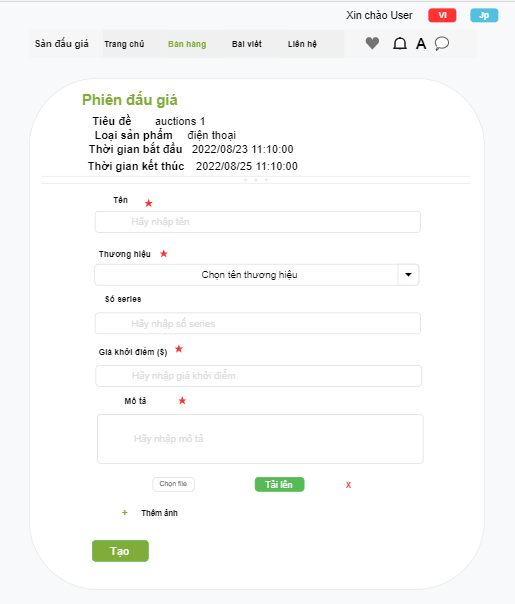
\includegraphics[width=10.04cm,height=11.76cm]{images/itemcreate.png}
    \caption{Mockup màn hình Tạo sản phẩm cho phiên đấu giá}
    \label{hinh410}
\end{figure}
Hình \ref{hinh410} mô tả mockup giao diện màn hình tạo sản phẩm cho một phiên đấu giá. Phía trên cùng là thông tin phiên đấu giá mà người dùng đang thêm sản phẩm. phía dưới là form để điền các thông tin của sản phẩm cần thêm. Đồng tiền được quy định chung cho website là \$
\begin{figure}[H]
    \centering
    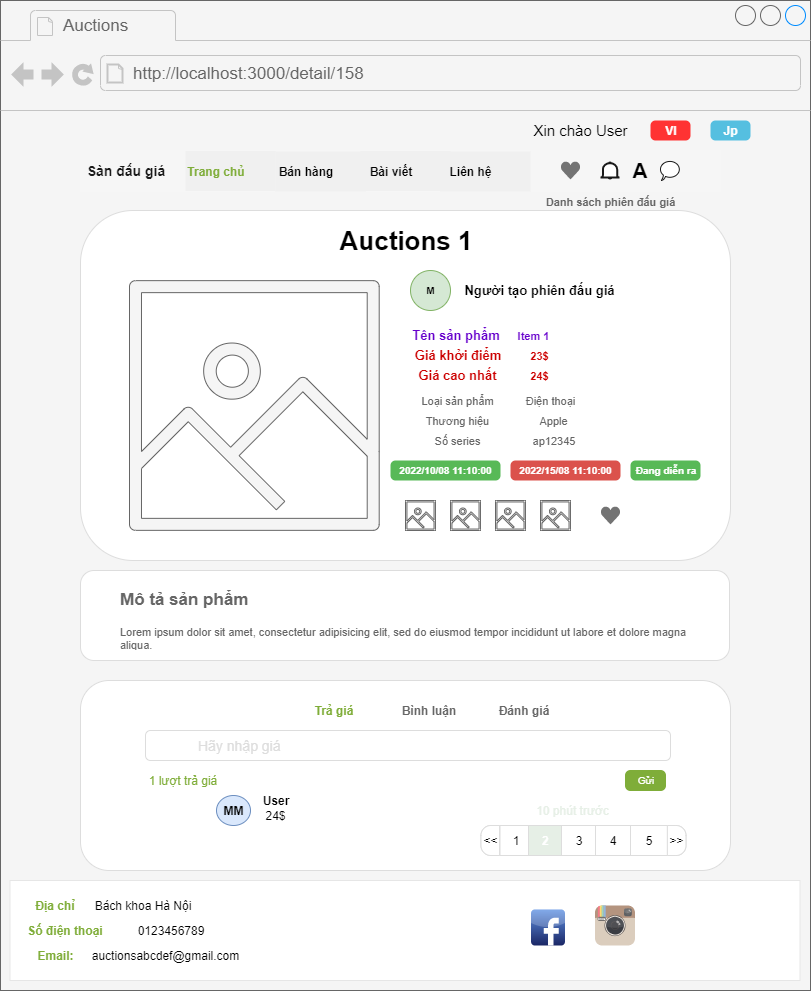
\includegraphics[width=10.04cm,height=11.76cm]{images/detailitem.png}
    \caption{Mockup màn hình Chi tiết phiên đấu giá}
    \label{hinh411}
\end{figure}
Hình \ref{hinh411} mô tả giao diện của màn hình chi tiết phiên đấu giá, bao gồm các hình ảnh, thông tin của sản phẩm, avatar, tên của người tạo phiên đấu giá. Phía dưới là các tab để trả giá, bình luận, đánh giá sản phẩm. 
\subsubsection{Thiết kế lớp}
\begin{figure}[H]
    \centering
    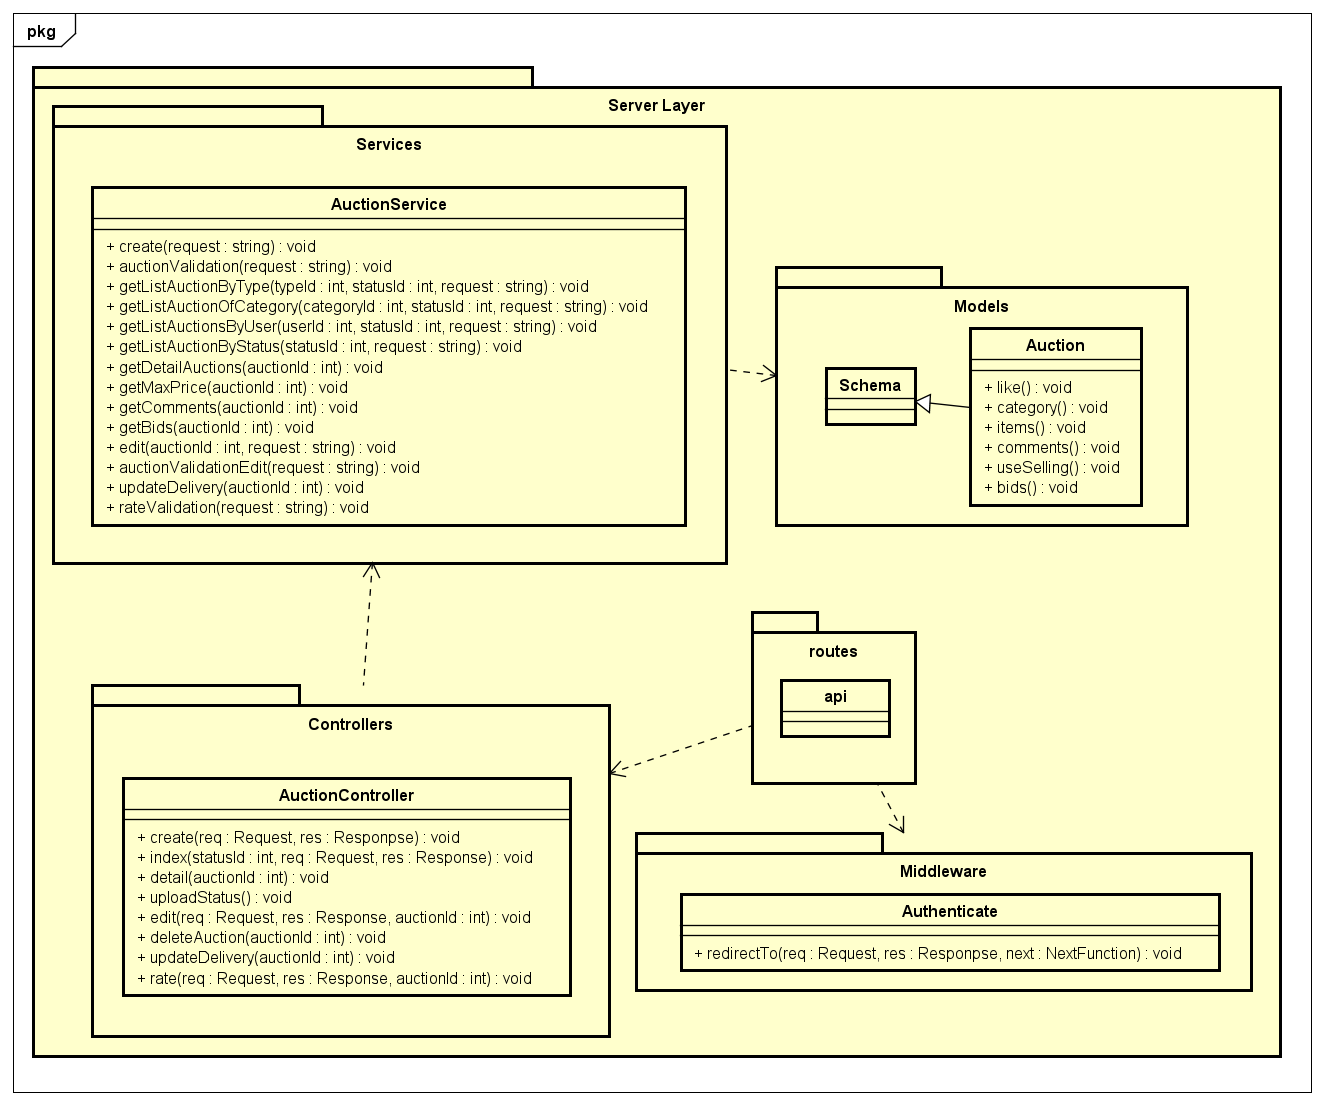
\includegraphics[width=11.4cm,height=9.54cm]{images/detailclass.png}
    \caption{Thiết kế lớp quản lý phiên đấu giá ( tạo, chỉnh sửa, xóa, cập nhật trạng thái, giao hàng, đánh giá)}
    \label{hinh412}
\end{figure}
\newpage

%\begin{table}[]
    %\centering
    \tablehead{%
    \hline
     \bfseries Tên phương thức & \bfseries Đầu vào & \bfseries Đầu ra & \bfseries Ý nghĩa  \\\hline}
    \tabletail{\hline}
    \topcaption{Bảng đặc tả lớp Authenticate}
    \label{bang43}
    \begin{supertabular}{| p{.20\textwidth} | p{.15\textwidth} | p{.15\textwidth} | p{.40\textwidth} |}
        \multicolumn{4}{|c|}{Lớp Authenticate}\\\hline
        redirectTo & {%
            \begin{tabular}{l}
                 Request\\
                 Response\\
                 NextFunction
            \end{tabular}
        }   & void &  Hàm xử lý request khi tài khoản người dùng cần phải đăng nhập thì mới được sử dụng các tác vụ sau. Nếu chưa đăng nhập thì trả message “Chưa đăng nhập”\\\hline
    \end{supertabular}\\
% \end{table}
%\begin{table}[H]
    %\centering
    \tablehead{%
    \hline
    \bfseries Tên phương thức & \bfseries Đầu vào & \bfseries Đầu ra & \bfseries Ý nghĩa  \\\hline}
    \tabletail{\hline}
    \topcaption{Bảng đặc tả lớp AuctionController}
    \label{bang44}
    \begin{supertabular}{| p{.20\textwidth} | p{.15\textwidth} | p{.15\textwidth} | p{.40\textwidth} |}
    \hline
        \multicolumn{4}{|c|}{Lớp AuctionController}\\\hline
        create & Request, Response & void & Hàm tạo phiên đấu giá\\\hline
        index & statusId, Request, Response & void & Hàm lấy ra danh sách phiên đấu giá theo trạng thái ( statusId)\\\hline
        detail & auctionId & void & Hàm lấy ra chi tiết phiên đấu giá\\\hline
        uploadStatus & & void & Hàm cập nhật trạng thái phiên đấu giá\\\hline
        edit & auctionId, Request, Response & void & Hàm chỉnh sửa phiên đấu giá chưa được duyệt\\\hline
        deleteAuction & auctionId & void & Hàm xóa phiên đấu giá chưa được duyệt\\\hline
        updateDelivery & auctionId & void & Hàm update tình trạng giao hàng\\\hline
        rate & auctionId, Request, Response & void & Hàm đánh giá sản phẩm phiên đấu giá\\\hline
    \end{supertabular}
%\end{table}
%\begin{table}[H]
    %\centering
    \tablehead{%
    \hline
    \bfseries Tên phương thức & \bfseries Đầu vào & \bfseries Đầu ra & \bfseries Ý nghĩa  \\\hline}
    \tabletail{\hline}
    \topcaption{Bảng đặc tả lớp AuctionService}
    \label{bang45}
    \begin{supertabular}{| p{.27\textwidth} | p{.15\textwidth} | p{.10\textwidth} | p{.38\textwidth} |} 
    \hline
        \multicolumn{4}{|c|}{Lớp AuctionService}\\\hline
        create & request & void & Hàm tạo phiên đấu giá\\\hline
        auctionValidation & request & void & Hàm để bắt các lỗi khi tạo phiên đấu giá\\\hline
        getListAuctionByType & typeId, satusId, request & void & Hàm lấy ra chi tiết phiên đấu giá theo trạng thái (statusId) và nhóm loại sản phẩm (typeId)\\\hline
        getListAuctionOfCategory & & categoryId, statusId, request & Hàm lấy ra chi tiết phiên đấu giá theo trạng thái (statusId) và loại sản phẩm (categoryId)\\\hline
        getListAuctionByUser & userId, satusId, request& void & Hàm lấy ra chi tiết phiên đấu giá theo trạng thái (statusId) và người dùng (userId)\\\hline
        getListAuctionStatus & statusId, request & void & Hàm lấy ra chi tiết phiên đấu giá theo trạng thái (statusId) trên toàn hệ thống\\\hline
        getDetailAuctions & auctionId & void & Chi tiết phiên đấu giá\\\hline
        getMaxPrice & auctionId & void & Hàm trả về lượt trả giá lớn nhất của phiên đấu giá\\\hline
        getComments & auctionId & void & Hàm trả về danh sách bình luận của phiên đấu giá\\\hline
        getBids & auctionId & void & Hàm trả ra danh sách trả giá của phiên đấu giá\\\hline
        getMaxPrice & auctionId, Request, Response & void & Hàm đánh giá sản phẩm phiên đấu giá\\\hline
        edit & auctionId, request & void & Hàm chỉnh sửa phiên đấu giá chưa được duyệt\\\hline
        auctionValidationEdit & request & void & Hàm bắt lỗi khi chỉnh sửa phiên đấu giá chưa được duyệt\\\hline
        updateDelivery & request & void & Cập nhật trạng thái giao hàng sản phẩm của phiên đấu giá\\\hline
        rateValidation & auctionId & void & Bắt lỗi khi đánh giá sản phẩm của phiên đấu giá sau khi nhận được hàng.\\\hline
    \end{supertabular}
%\end{table}
%\begin{table}[H]
    %\centering
    \tablehead{%
    \hline
    \bfseries Tên phương thức & \bfseries Đầu vào & \bfseries Đầu ra & \bfseries Ý nghĩa  \\\hline}
    \tabletail{\hline}
    \topcaption{Bảng đặc tả lớp Auction}
    \label{bang46}
    \begin{supertabular}{| p{.20\textwidth} | p{.15\textwidth} | p{.15\textwidth} | p{.40\textwidth} |} 
    \hline
        \multicolumn{4}{|c|}{Lớp Auction}\\\hline
        like & & void & Hàm trả định nghĩa quan hệ giữa bảng auctions và favorites\\\hline
        category & & void & Hàm định nghĩa quan hệ giữa bảng auctions và categories\\\hline
        items & & void & Hàm trả định nghĩa quan hệ giữa bảng auctions và items\\\hline
        comments & & void & Hàm trả định nghĩa quan hệ giữa bảng auctions và comments\\\hline
        useSelling & & void & Hàm trả định nghĩa quan hệ giữa bảng auctions và users\\\hline
        bids & & void & Hàm trả định nghĩa quan hệ giữa bảng auctions và bids\\\hline
    \end{supertabular}
%\end{table}
\subsubsection{Thiết kế API}
Phần này sẽ liệt kê danh sách các API sử dụng trong hệ thống.
%\begin{table}[H]
    %\centering
    \tablehead{%
    \hline
    \bfseries STT & \bfseries Mục đích & \bfseries Phương thức & \bfseries Địa chỉ  \\\hline}
    \tabletail{\hline}
    \topcaption{Danh sách API}
    \label{bang47}
    \begin{supertabular}{| p{.05\textwidth} | p{.35\textwidth} | p{.10\textwidth} | p{.40\textwidth} |} 
    \hline
        1 & Đăng nhập & POST & /api/login\\\hline
        2 & Đăng ký & POST & /api/signup\\\hline
        3 & Chỉnh sửa tài khoản & POST & /api/edit\\\hline
        4 & Thay đổi mật khẩu & POST & /api/changepass\\\hline
        5 & Đăng xuất & POST & /api/logout\\\hline
        6 & Thông tin tài khoản & GET & /api/info\\\hline
        7 & Danh sách phiên đấu giá & GET & /api/auctions/{statusId}\\\hline
        8 & Chi tiết phiên đấu giá & GET & /api/auctions/detail/{auctionId}\\\hline
        9 & Tạo phiên đấu giá & POST & /api/auctions/create\\\hline
        10 & Chỉnh sửa phiên đấu giá chưa được duyệt & POST & /api/auctions/edit/{auctionId}\\\hline
        11 & Xóa phiên đấu giá chưa được duyệt & POST & /api/auctions/deleteAuction/{auctionId}\\\hline
        12 & Thêm sản phẩm cho phiên đấu giá & POST & /api/items/create/{auctionId}\\\hline
        13 & Chỉnh sửa sản phẩm của phiên đấu giá chưa được duyệt & POST & /api/items/edit/{auctionId}\\\hline
        14 & Danh sách bình luận của phiên đấu giá & GET & /api/comments/{auctionId}\\\hline
        15 & Bình luận & POST & /api/comments/create/{auctionId}\\\hline
        16 & Xóa bình luận & POST & /api/comments/delete/{commentId}\\\hline
        17 & Danh sách lượt trả giá của phiên đấu giá & GET & /api/bids/{auctionId}\\\hline
        18 & Trả giá & POST & /api/bids/create/{auctionId}\\\hline
        19 & Cập nhật trạng thái giao hàng & POST & /api/updateDelivery/{auctionId}\\\hline
        20 & Đánh giá khi nhận được hàng & POST & /api/auctions/rate/{auctionId}\\\hline
        21 & Danh sách đánh giá & GET & /api/rates/{auctionId}\\\hline
        22 & Danh sách loại sản phẩm & GET & /api/categories\\\hline
        23 & Danh sách thương hiệu & GET & /api/brands\\\hline
        24 & Chấp nhận giá cao nhất khi phiên đấu giá kết thúc & POST & /api/accept/{auctionId}\\\hline
        26 & Thích, không thích phiên đấu giá & POST & /api/updateLike/{auctionId}\\\hline
        27 & Danh sách phiên đấu giá yêu thích & GET & /api/likes/{statusId}\\\hline
        28 & Danh sách tin tức & GET & /api/news\\\hline
        29 & Đọc tin tức & POST & /api/news/read/{newId}\\\hline
        30 & Danh sách thông báo phiên đấu giá bị từ chối & GET& /api/notifications \\\hline
        31 & Đọc thông báo & POST& /api/notifications/read/{auctionDenyId}\\\hline
        32 & Xóa thông báo& POST & /api/notifications/{auctionId}\\\hline
        33 & Slide trang chủ& POST& /api/slider\\\hline
        34 & Tìm kiếm& GET& /api/search\\\hline
        35 & Danh sách cuộc nói chuyên & GET & /api/chat\\\hline
        36 & Tạo cuộc nói chuyện mới & POST & /api/chat/conversation/{useReceived}\\\hline
        37 & Tạo tin nhắn& POST& /api/chat/message/{chatId}\\\hline
        38 & Danh sách tin nhắn của cuộc nói chuyên & GET&  /api/chat/listMessage/{chatId}\\\hline
        39 & Cập nhật trạng thái phiên đấu giá & GET & /api/auctions/update/status\\\hline
    \end{supertabular}
%\end{table}
\subsubsection{Thiết kế cơ sở dữ liệu}
\begin{figure}[H]
    \centering
    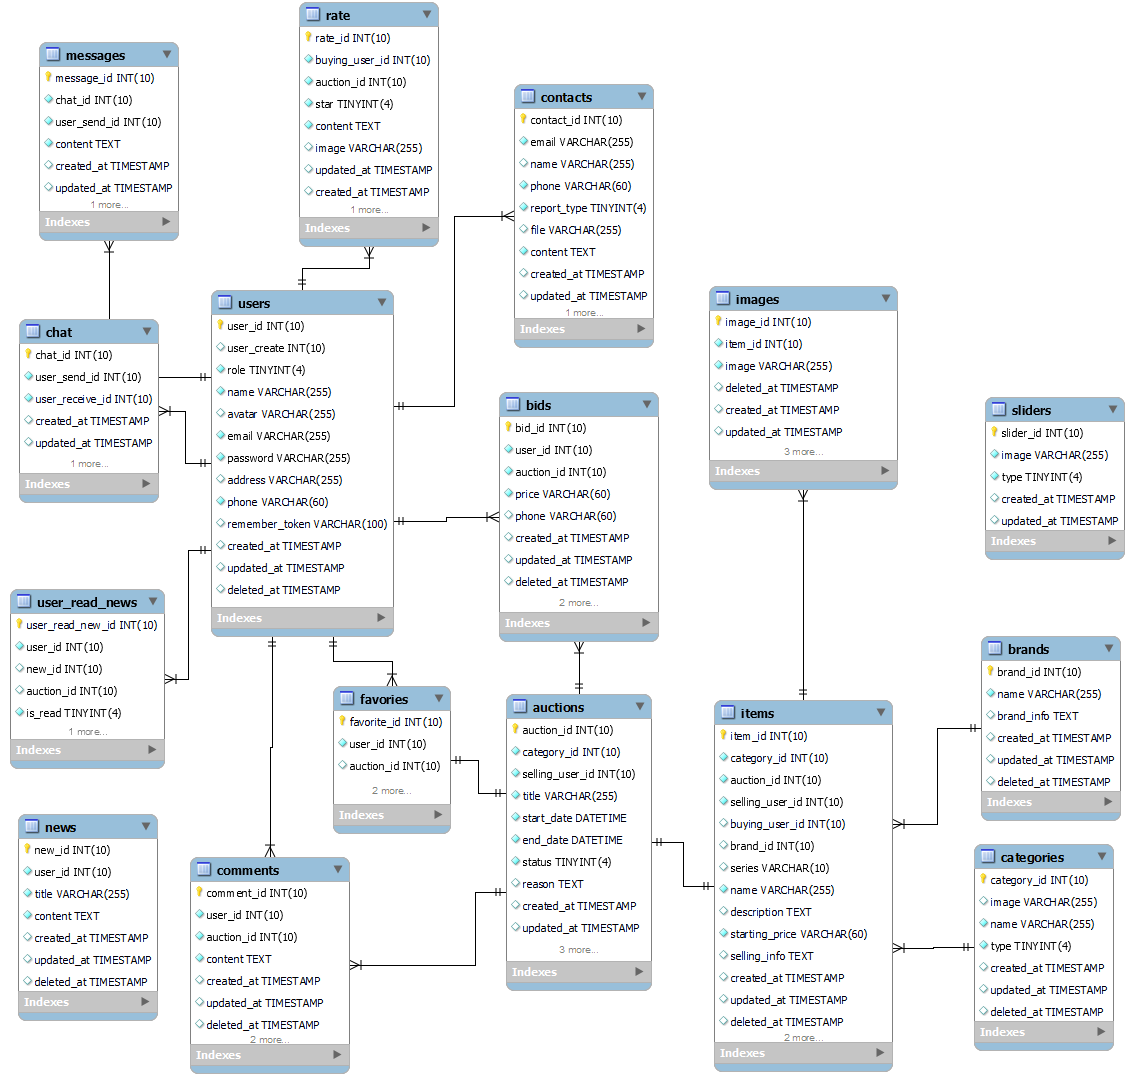
\includegraphics[width=11.4cm,height=11.0cm]{images/database.png}
    \caption{Sơ đồ thực thể liên kết}
    \label{hinh413}
\end{figure}
Hình \ref{hinh413} là sơ đồ thực thể liên kết cho cơ sở dữ liệu của hệ thống đấu giá trực tuyến. Ý nghĩa của từng thực thể được mô tả trong Bảng 4.8.
%\begin{table}[H]
    %\centering
    \tablehead{%
    \hline
    \bfseries Tên thực thể & \bfseries Ý nghĩa\\\hline}
    \tabletail{\hline}
    \topcaption{Ý nghĩa các thực thể}
    \label{bang48}
    \begin{supertabular}{| p{.30\textwidth} | p{.60\textwidth} |} 
    \hline
        auctions & Phiên đấu giá\\\hline
        users & Tài khoản người dùng\\\hline
        comments & Danh sách bình luận của phiên đấu giá\\\hline
        bids& Danh sách lượt trả giá của phiên đấu giá\\\hline
        items& Sản phẩm của phiên đấu giá\\\hline
        categories& Loại sản phẩm\\\hline
        brands& Thương hiệu sản phẩm\\\hline
        images& Danh sách hình ảnh của sản phẩm\\\hline
        favorites& Thích, không thích phiên đấu giá\\\hline
        contacts& Liên lạc với Quản tri viên\\\hline
        news& Tin tức\\\hline
        user\_read\_news& Tài khoản đã đọc tin tức chưa\\\hline
        chat& Danh sách cuộc nói chuyện\\\hline
        messages& Danh sách tin nhắn\\\hline
        rate& Danh sách đánh giá cho phiên đấu giá\\\hline
        slides & Danh sách slide hiển thị trên trang chủ client\\\hline
    \end{supertabular}
%\end{table}
\subsection{Xây dựng ứng dụng}
\subsubsection{Thư viện và công cụ sử dụng}
%\begin{table}[H]
    %\centering
    \tablehead{%
    \hline
    \bfseries Mục đích & \bfseries Công cụ &\bfseries Địa chỉ URL\\\hline}
    \tabletail{\hline}
    \topcaption{Danh sách thư viện và công cụ sử dụng}
    \label{bang49}
    \begin{supertabular}{| p{.30\textwidth} | p{.25\textwidth} | p{.35\textwidth} |} 
    \hline
        IDE lập trình& Visual Studio Code& https://code.visualstudio.com \\\hline
        Ngôn ngữ lập trình& Javascript& https://www.javascript.com \\\hline
        Xây dựng giao diện& HTML&https://developer.mozilla.org/en-US/docs/Web/HTML \\\hline
        Xây dựng giao diện& CSS& https://developer.mozilla.org/en-US/docs/Web/CSS \\\hline
        Quản trị CSDL& MySQL& https://www.mysql.com \\\hline
        Backend& PHP 7.1.32& https://www.php.net\\\hline
        Backend Framework& Laravel 8.x& https://laravel.com \\\hline
        Web UI Library& ReactJs 18.0.0&https://reactjs.org/\\\hline
                      & Material UI 5.6.1&https://mui.com \\\hline
        Phân tích thiết kế& Astah 8.5.0 & https://astah.net/ \\\hline
                          & Diagram editor& https://www.diagrameditor.com/ \\\hline
    \end{supertabular}
%\end{table}
\subsubsection{Kết quả đạt được}
Từ những tìm hiểu và phân tích trên em đã xây dựng Website đấu giá trực tuyến với các module chính: (i) Tìm kiếm, (ii) xem chi tiết phiên đấu giá, (iii) tạo phiên đấu giá, (iv) tham gia phiên đấu giá ( trả giá, bình luận, đánh giá), (v) nhắn tin, (vi) yêu thích phiên đấu giá, (vii) xem tin tức, (viii) xem thông báo từ chối phiên đấu giá. Về hệ thống quản lý phía Quản trị viên là quản lý phê duyệt phiên đấu giá, quản lý việc thêm sửa xóa loại sản phẩm, thương hiệu, slide, tin tức.
%\begin{table}[H]
    %\centering
    \tablehead{%
    \hline
    \bfseries Thông tin & \bfseries Thống kê\\\hline}
    \tabletail{\hline}
    \topcaption{Thống kê thông tin ứng dụng server phía Người dùng}
    \label{bang410}
    \begin{supertabular}{| p{.45\textwidth}| p{.45\textwidth} |} 
    \hline
        Số dòng code& 4933\\\hline
        Dung lượng mã nguồn&233KB \\\hline
        Môi trường lập trình&Dell Vostro \\\hline
        Công cụ kiểm thử & Postman\\\hline
        Số bảng trong cơ sở dữ liệu  &16 bảng \\\hline
    \end{supertabular}
%\end{table}
%\begin{table}[H]
    %\centering
    \tablehead{%
    \hline
    \bfseries Thông tin & \bfseries Thống kê\\\hline}
    \tabletail{\hline}
    \topcaption{Thống kê thông tin ứng dụng web}
    \label{bang411}
    \begin{supertabular}{| p{.45\textwidth}| p{.45\textwidth} |} 
    \hline
        Số dòng code& 8265\\\hline
        Dung lượng mã nguồn&950KB \\\hline
        Môi trường lập trình&Dell Vostro \\\hline
        Công cụ kiểm thử & Chrome Browser, Microsoft Edge\\\hline
    \end{supertabular}
%\end{table}
%\begin{table}[H]
    %\centering
    \tablehead{%
    \hline
    \bfseries Thông tin & \bfseries Thống kê\\\hline}
    \tabletail{\hline}
    \topcaption{Thống kê thông tin ứng dụng phía Quản trị viên}
    \label{bang412}
    \begin{supertabular}{| p{.45\textwidth}| p{.45\textwidth} |} 
    \hline
        Số dòng code& 5077\\\hline
        Dung lượng mã nguồn&295KB \\\hline
        Môi trường lập trình&Dell Vostro \\\hline
        Công cụ kiểm thử & Chrome Browser, Microsoft Edge\\\hline
    \end{supertabular}
%\end{table}
\subsubsection{Minh họa các chức năng chính}
\begin{figure}[H]
    \centering
    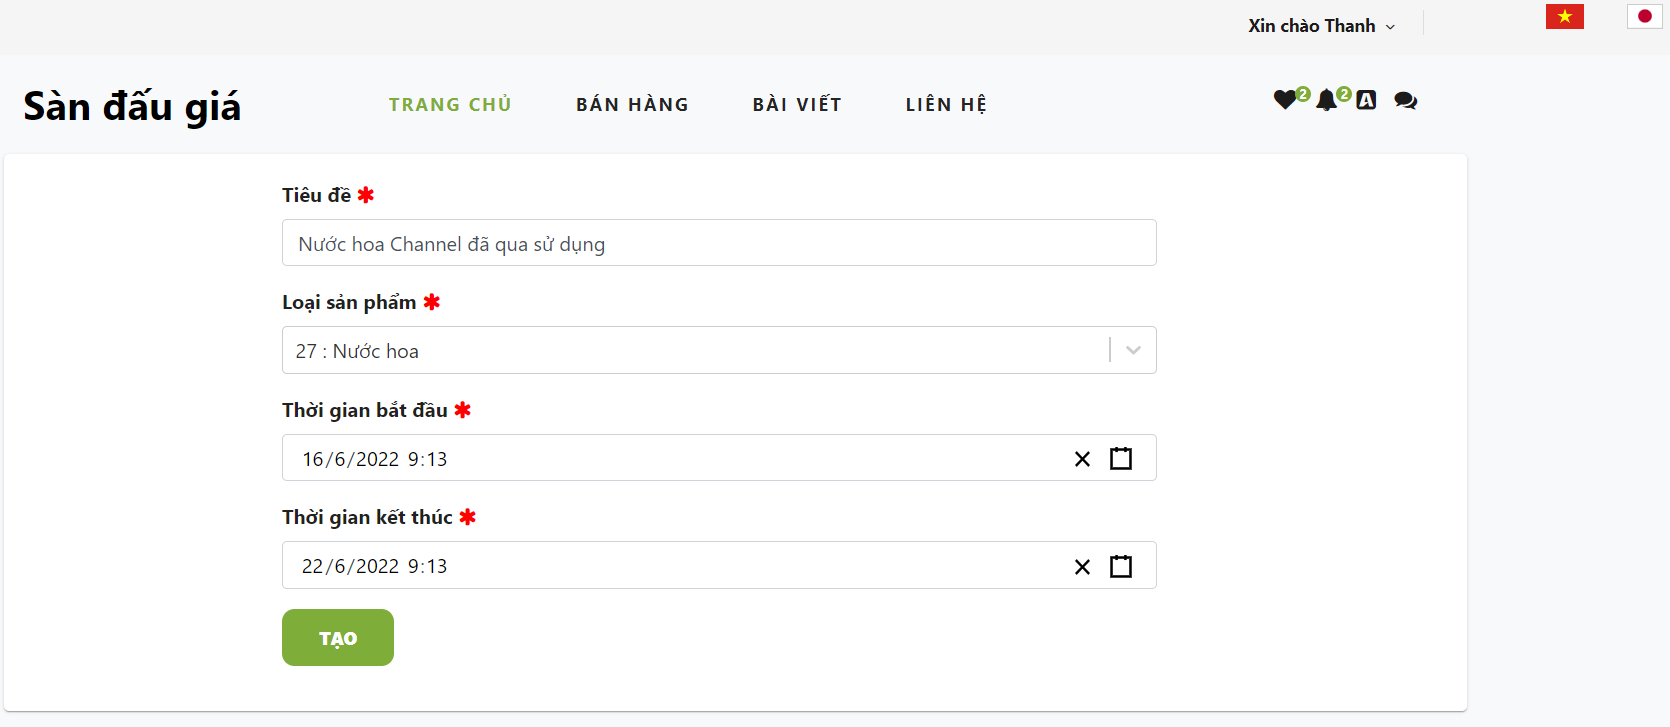
\includegraphics[width=11.4cm,height=4.95cm]{images/createauctiondemo.png}
    \caption{Giao diện tạo phiên đấu giá}
    \label{hinh414}
\end{figure}
Hình\ref{hinh414} mô tả màn hình tạo phiên đấu giá. Người dùng đã có tài khoản thì có quyền được tạo phiên đấu giá. Người dùng nhập các thông tin cần thiết trên màn hình, những trường nào có dấu sao màu đỏ là những trường bắt buộc phải nhập. Nếu người dùng không nhập hay nhập sai định dạng thông tin thì hệ thống sẽ báo lỗi tương ứng phía dưới ô đó. 
\begin{figure}[H]
    \centering
    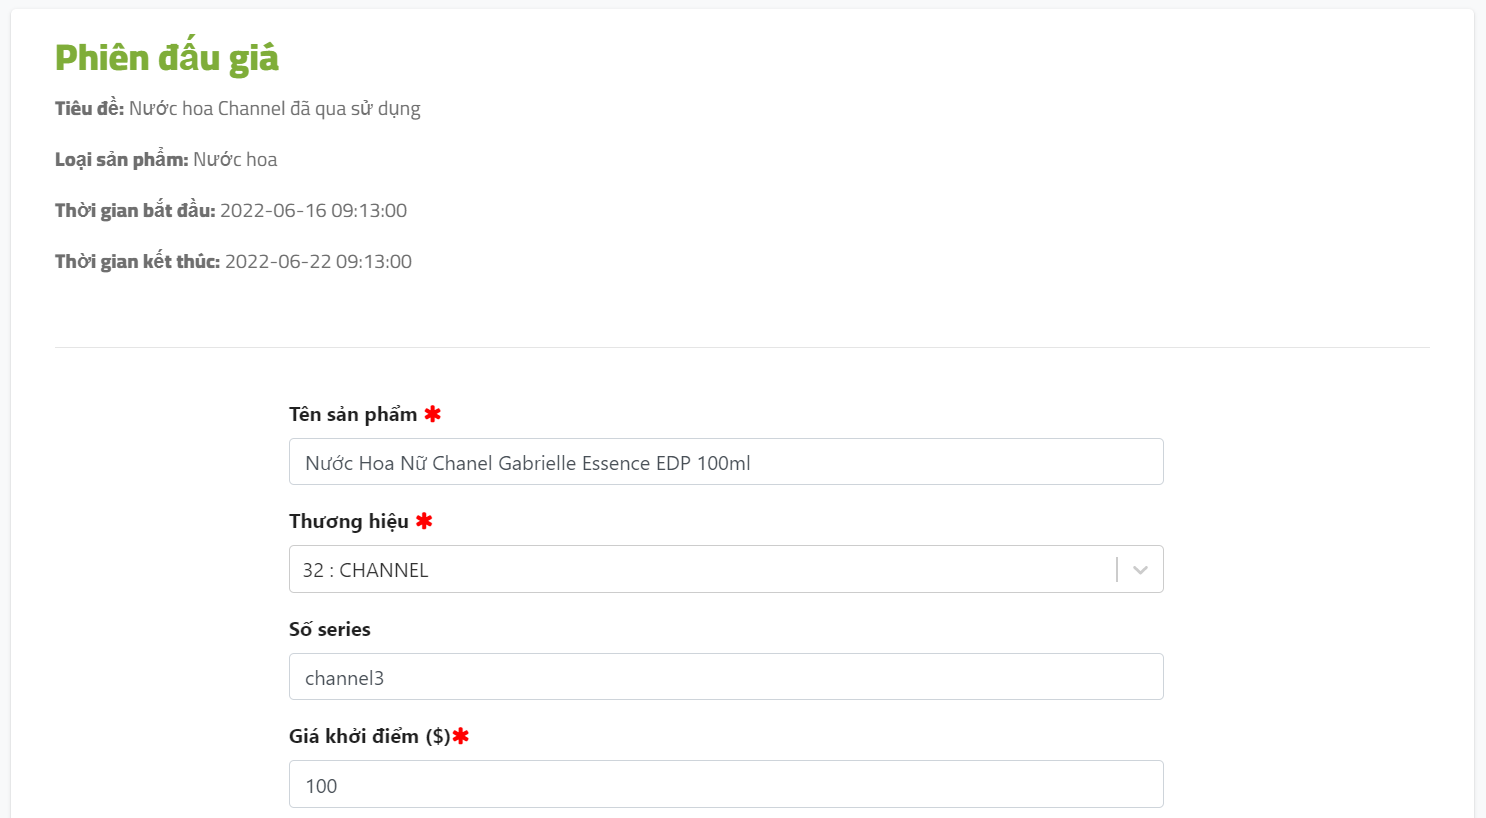
\includegraphics[width=11.4cm,height=6.28cm]{images/createitem1demo.png}
    \label{hinh4151}
\end{figure}
\begin{figure}[H]
    \centering
    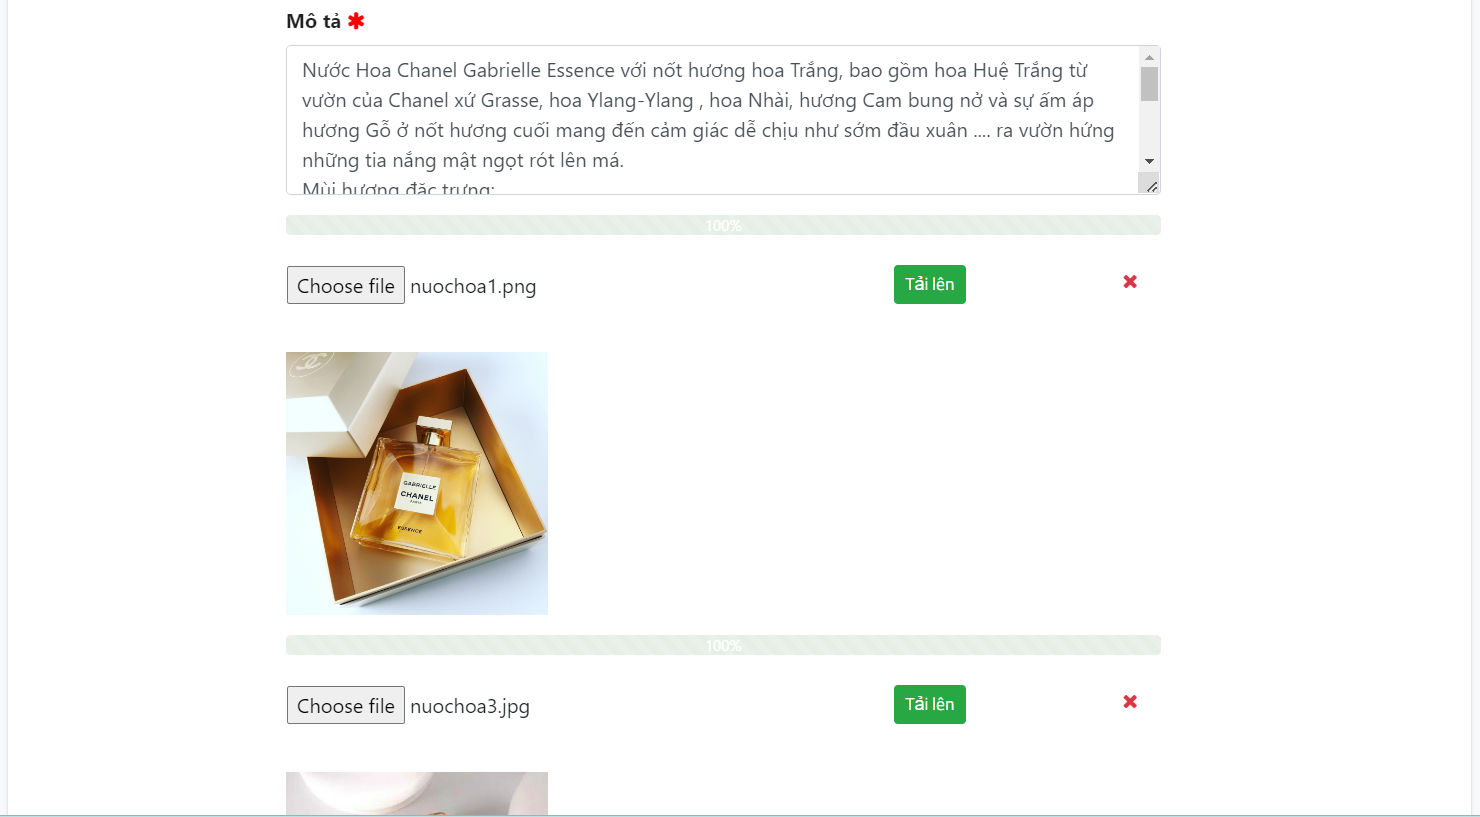
\includegraphics[width=11.4cm,height=6.32cm]{images/createitem2demo.png}
    \caption{Giao diện tạo sản phẩm cho phiên đấu giá.}
    \label{hinh415}
\end{figure}
Hình \ref{hinh415} mô tả giao diện tạo sản phẩm cho phiên đấu giá. Người dùng sau khi tạo phiên đấu giá thì có thể thêm sản phẩm vào phiên đấu giá đó. Thông tin của phiên đấu giá được để lên đầu form tạo sản phẩm. Người dùng nhập các thông tin sản phẩm cần thiết. Nếu không nhập hay nhập sai thông tin thì hệ thống sẽ báo lỗi phía dưới trường đó.
\begin{figure}[H]
    \centering
    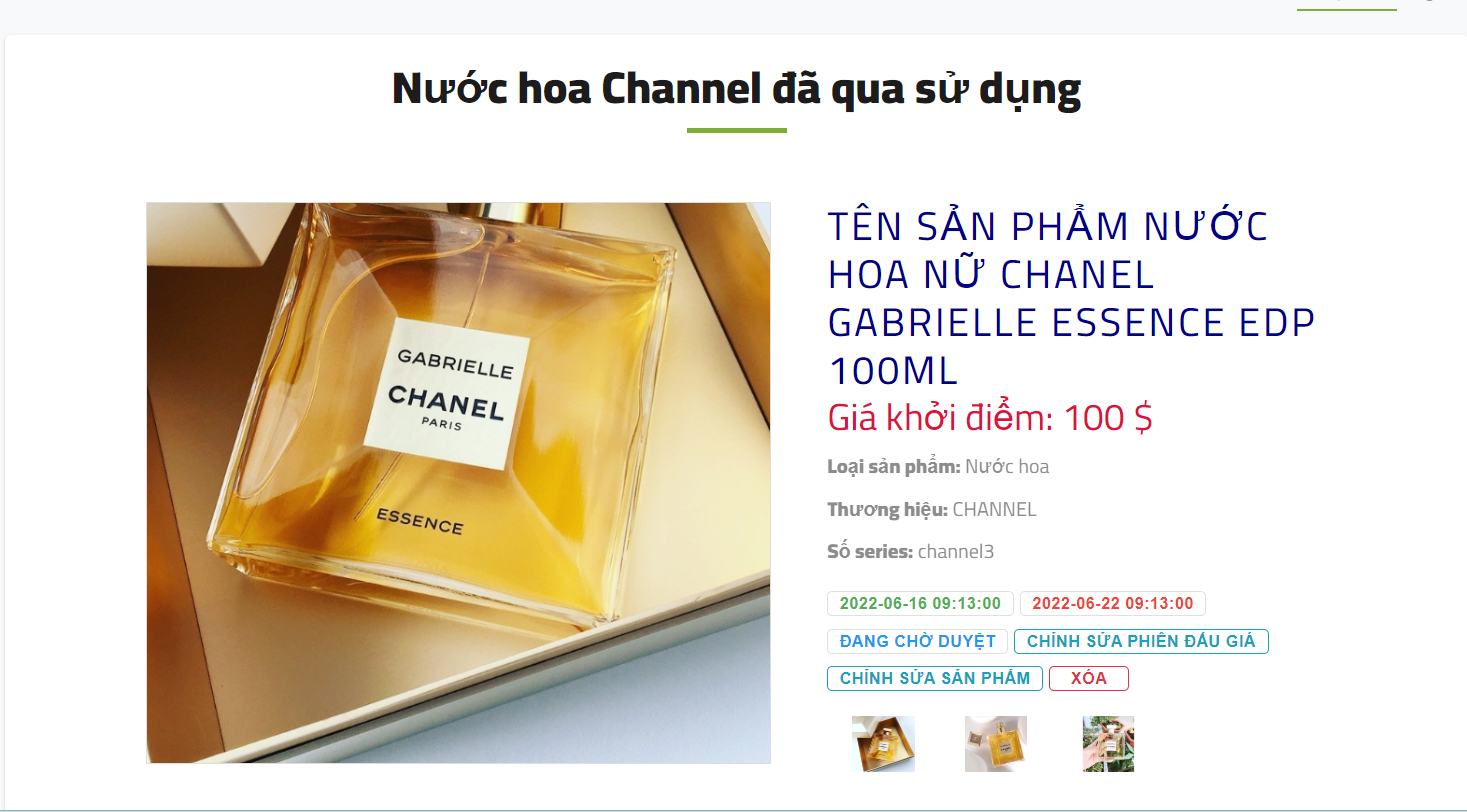
\includegraphics[width=11.4cm,height=6.32cm]{images/auctionwait.png}
    \caption{Giao diện phiên đấu giá vừa tạo đang chờ duyệt.}
    \label{hinh416}
\end{figure}
Hình \ref{hinh416} mô tả giao diện phiên đấu giá vừa tạo đang chờ admin duyệt. Sau khi người dùng tạo phiên đấu giá và sản phẩm thì trong trang cá nhân của Người dùng sẽ hiển thị thông tin phiên đấu giá vừa tạo (bao gồm: tiêu đề phiên đấu giá đặt trên cùng, hình ảnh sản phẩm, sau đó là tên sản phẩm, giá khởi điểm, loại sản phẩm, thương hiệu, số series, label màu xanh thể hiện thời gian bắt đầu, màu đỏ thể hiện thời gian kết thúc và các button liên quan).\\
Trong trường hợp Người dùng tạo phiên đấu giá mà chưa thêm sản phẩm thì hệ thống hiển thị button Thêm sản phẩm, còn nếu đã Thêm sản phẩm rồi màn hình hiển thị các button chỉnh sửa, xóa phiên đấu giá đó. 
\begin{figure}[H]
    \centering
    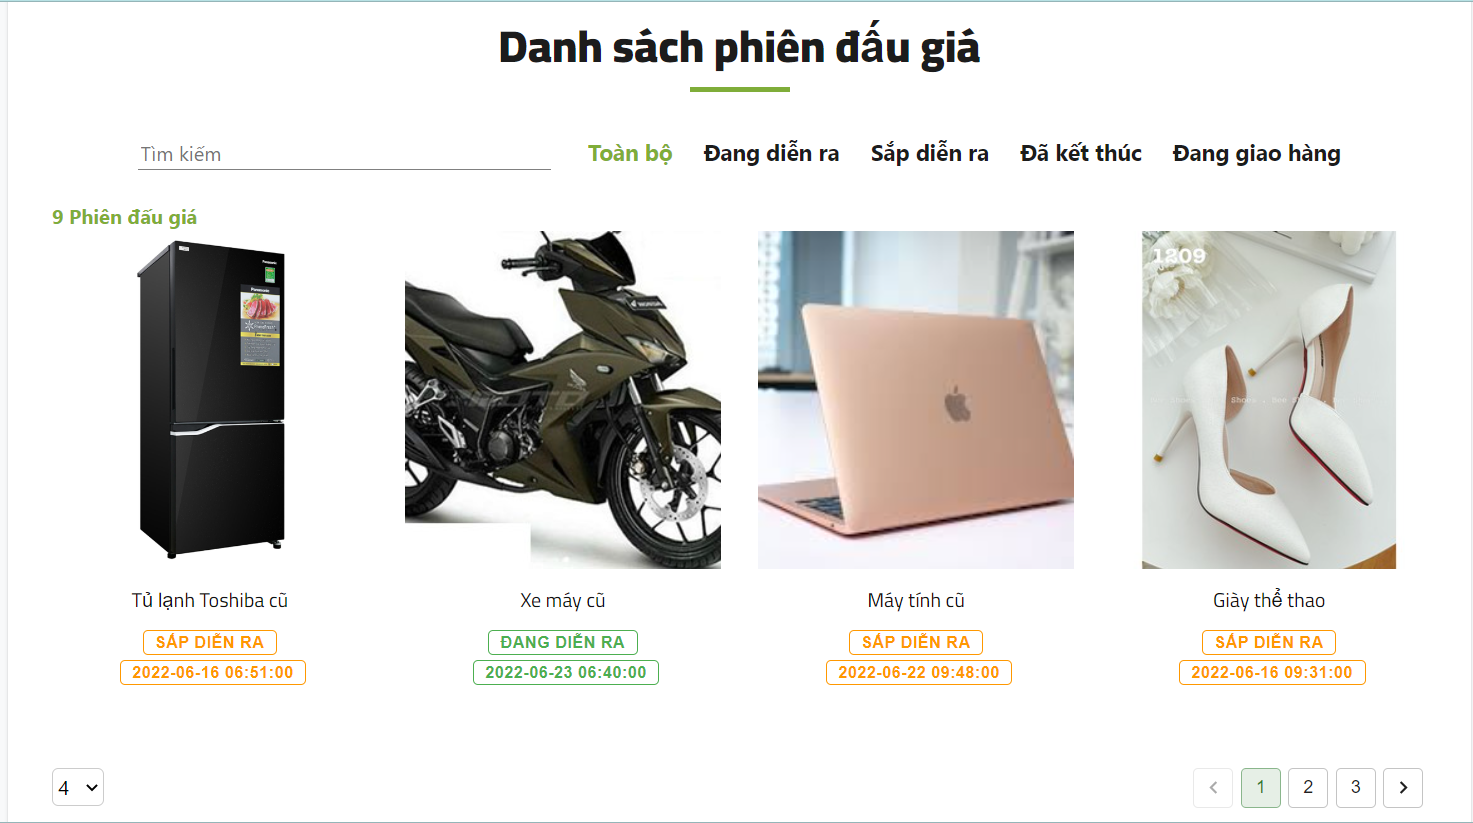
\includegraphics[width=11.4cm,height=6.36cm]{images/listauctions.png}
    \caption{Giao diện danh sách phiên đấu giá toàn hệ thống}
    \label{hinh417}
\end{figure}
Hình \ref{hinh417} mô tả giao diện danh sách phiên đấu giá trên toàn hệ thống. Màn hình hiển thị các trạng thái, tổng số phiên đấu giá ở trạng thái đó, tên của phiên đấu giá, thời gian bắt đầu, thời gian kết thúc. Với các phiên đấu giá đang diễn ra, đã kết thúc sẽ hiển thị thời gian kết thúc, còn riêng đối với phiên đấu giá sắp diễn ra thì hiển thị thời gian bắt đầu. Màu sắc của các label được hiển thị theo trạng thái của phiên đấu giá đó. Hình ảnh đại diện là hình ảnh của loại sản phẩm thuộc phiên đấu giá đó. Mỗi trang có thể chọn hiển thị 4, 8, 12, 24 phiên đấu giá. Tại đây cũng có thể tìm kiếm phiên đấu giá theo tên, ngày giờ. 
\begin{figure}[H]
    \centering
    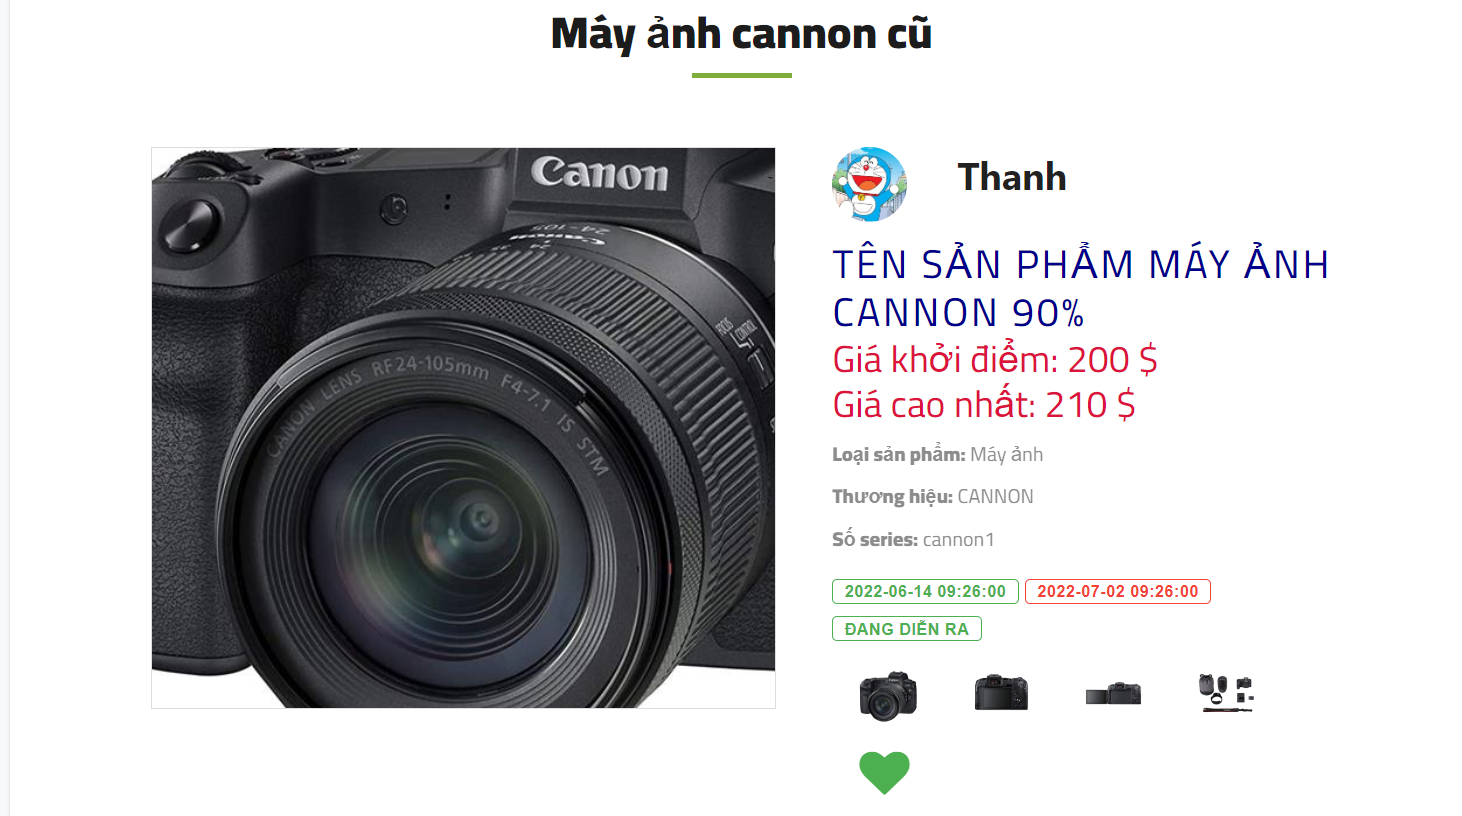
\includegraphics[width=11.4cm,height=6.36cm]{images/auctionactive.png}
    \caption{Giao diện chi tiết phiên đấu giá đang diễn ra}
    \label{hinh418}
\end{figure}
Hình \ref{hinh418} mô tả giao diện chi tiết phiên đấu giá đang diễn ra. Giao diện này sẽ hiển thị tên phiên đấu giá ở trên cùng, tiếp đến là thông tin người bán, thông tin sản phẩm, trả giá cao nhất hiện tại, các hình ảnh của sản phẩm và icon trái tim để biết người dùng có yêu thích phiên đấu giá này không.
\begin{figure}[H]
    \centering
    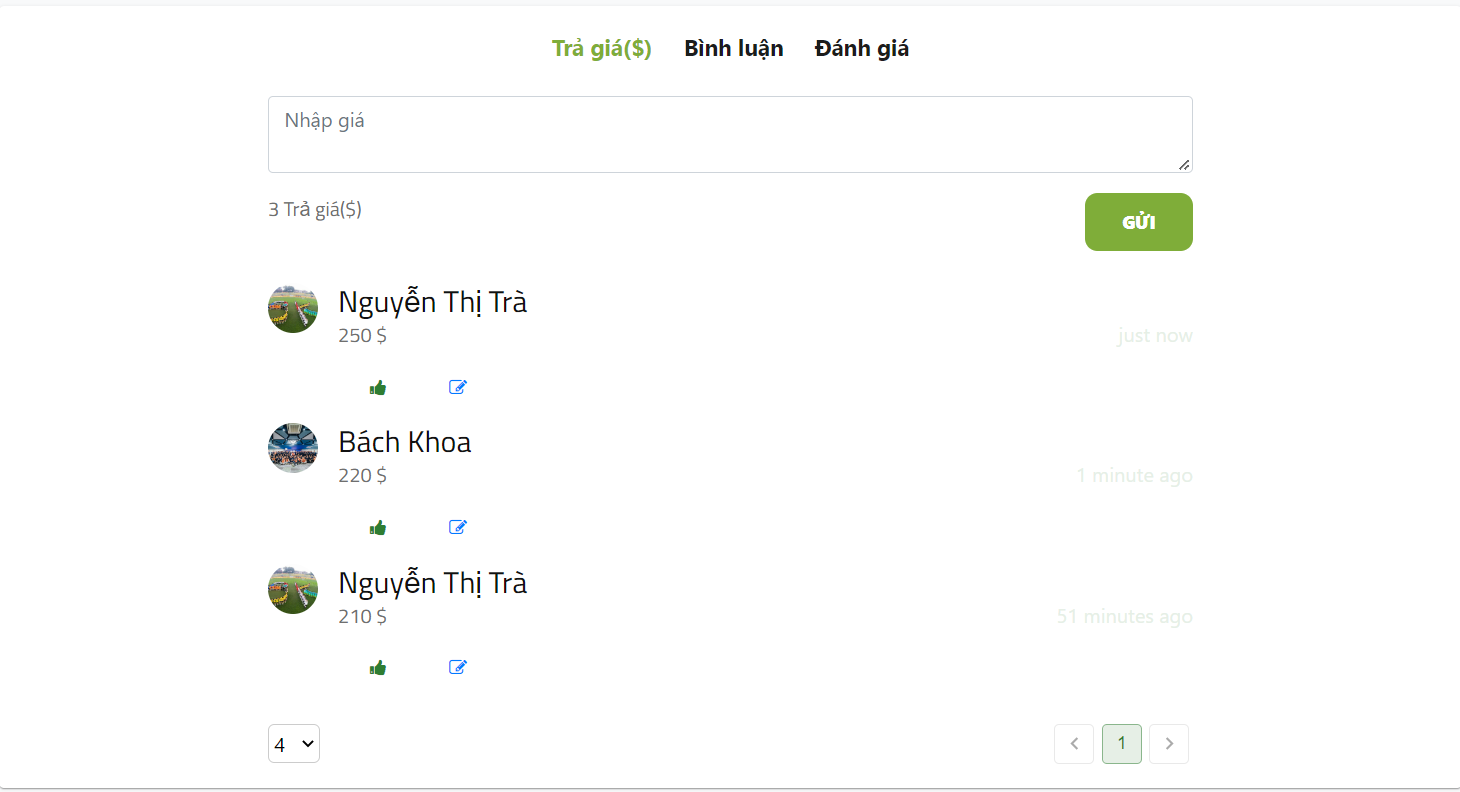
\includegraphics[width=11.4cm,height=6.20cm]{images/commentbid.png}
    \caption{Giao diện các tab trả giá, bình luận, đánh giá của phiên đấu giá.}
    \label{hinh419}
\end{figure}
Hình \ref{hinh419} mô tả giao diện các tab trả giá, bình luận, đánh giá của phiên đánh giá. Giao diện này sẽ hiển thị người thực hiện hành động, nội dung hành động, thời gian tạo và tổng số lượt trả giá, bình luận hay đánh giá đang có của phiên đấu giá. 
\begin{figure}[H]
    \centering
    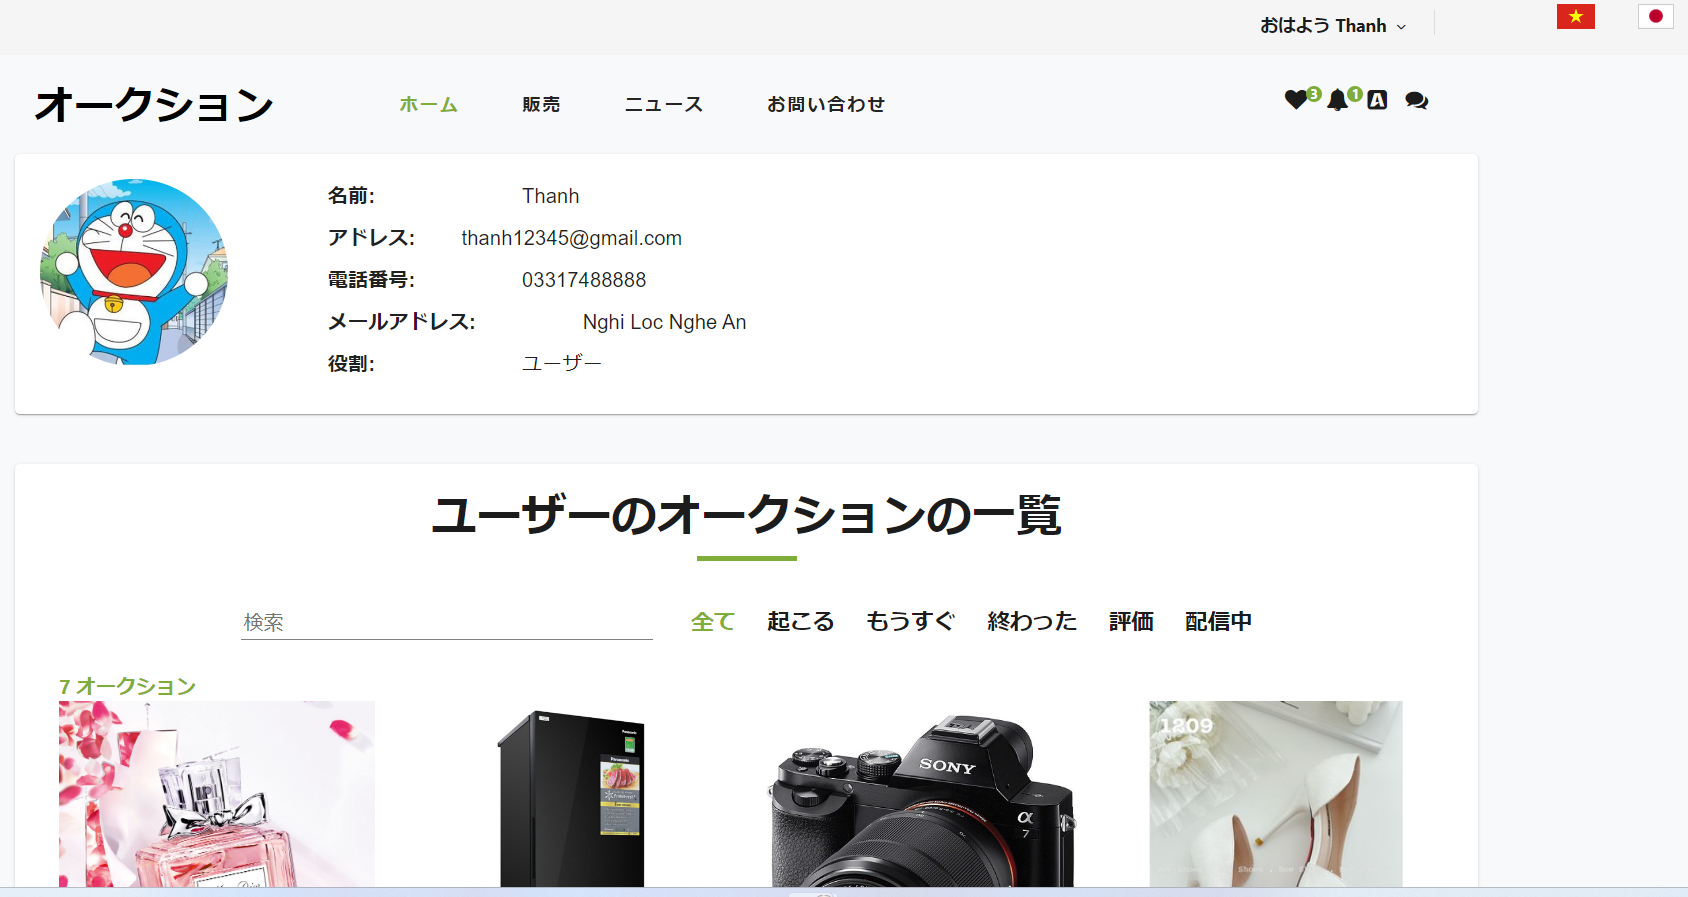
\includegraphics[width=11.4cm,height=6.06cm]{images/jp.png}
    \caption{Giao diện khi sử dụng ngôn ngữ là Tiếng Việt}
    \label{hinh420}
\end{figure}
Hình \ref{hinh420} mô tả giao diện khi sử dụng ngôn ngữ tiếng Việt. Khi người dùng chọn vào lá cờ Việt Nam thì ngôn ngữ trên hệ thống chuyển toàn bộ qua tiếng Việt. Tuy nhiên hiện tại hệ thống chỉ chuyển đổi những tiêu đề đã có sẵn trong hệ thống, còn thông tin người dùng nhập bằng ngôn ngữ nào thì vẫn giữ nguyên đó.
\begin{figure}[H]
    \centering
    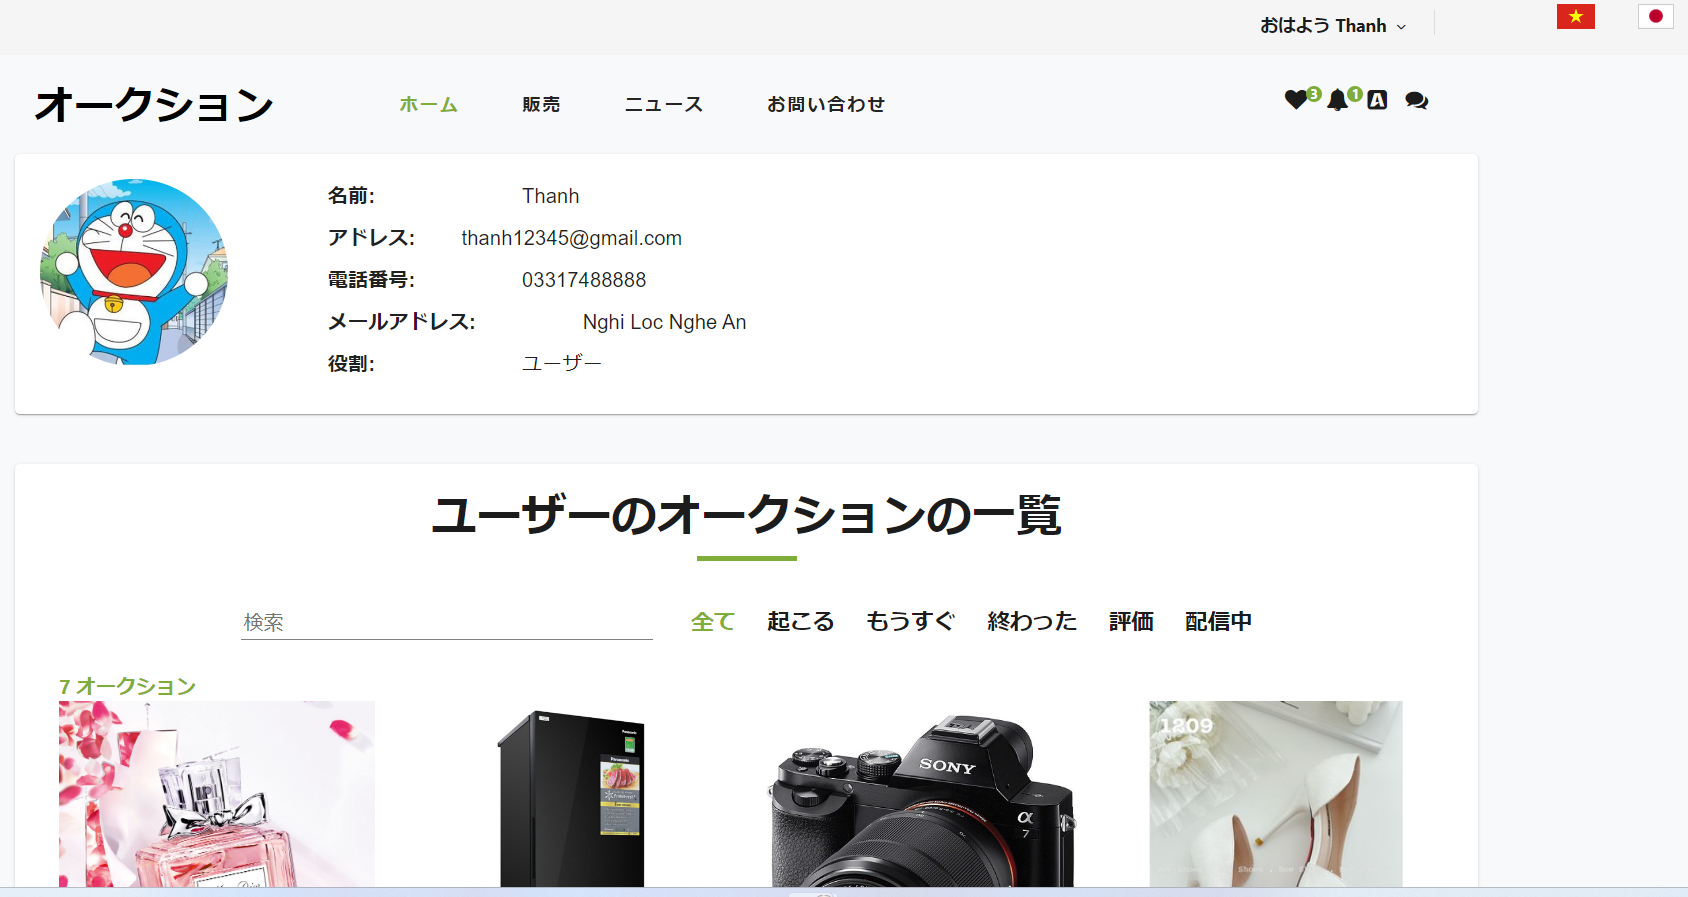
\includegraphics[width=11.4cm,height=6.06cm]{images/jp.png}
    \caption{Giao diện khi chuyển ngôn ngữ qua tiếng Nhật}
    \label{hinh421}
\end{figure}
Khi người dùng chọn vào lá cờ Nhật Bản thì ngôn ngữ trên hệ thống chuyển toàn bộ qua tiếng Nhật.
\subsection{Kiểm thử}
Để kiểm thử lại website đấu giá trực tuyến, sau khi kiểm thử API bằng Postman, ghép API hoàn chỉnh thì thực hiện bước kiểm thử sản phẩm sau cùng bằng kỹ thuật Black-Box trên môi trường Chrome browser, Microsoft Edge. Chi tiết kiểm thử một số chức năng được mô tả phía dưới. 
\subsubsection{Kiểm thử chức năng tạo phiên đấu giá}
\newpage
%\begin{table}[H]
    %\centering
    \tablehead{%
    \hline
    \bfseries Đầu vào & \bfseries Đầu ra & \bfseries Kết quả\\\hline}
    \tabletail{\hline}
    \topcaption{Kiểm thử chức năng tạo phiên đấu giá}
    \label{bang413}
    \begin{supertabular}{| p{.45\textwidth}|p{.30\textwidth}|p{.15\textwidth}|} 
    \hline
        Bỏ trống “Tiêu đề”
        Không chọn “Loại sản phẩm”
        Không chọn “Thời gian bắt đầu”
        Không chọn  “Thời gian kết thúc”
        & Thông báo lỗi “Yêu cầu nhập” ở dưới trường bị bỏ trống&Đạt \\\hline
        Nhập “Tiêu đề” quá 255 ký tự
        & Thông báo lỗi “Tối đa 255 ký tự “&Đạt \\\hline
        Không nhập “Thời gian bắt đầu”  ít nhất phải bắt đầu từ thời điểm hiện tại ngày hôm sau
        & Thông báo lỗi “ Thời gian bắt đầu sớm nhất từ ngày mai”&Đạt \\\hline
        Nhập “Thời gian kết thúc” sớm hơn “Thời gian bắt đầu”
        & Thông báo lỗi “Thời gian kết thúc phải sau thời gian bắt đầu”&Đạt \\\hline
        Nhập “Thời gian bắt đầu” và “Thời gian kết thúc” không đúng định dạng ngày tháng
        & Thông báo lỗi “Không đúng định dạng”&Đạt \\\hline
    \end{supertabular}
%\end{table}
\subsubsection{Kiểm thử chức năng tạo sản phẩm cho phiên đấu giá}
%\begin{table}[H]
    %\centering
    \tablehead{%
    \hline
    \bfseries Đầu vào & \bfseries Đầu ra & \bfseries Kết quả\\\hline}
    \tabletail{\hline}
    \topcaption{Kiểm thử chức năng tạo sản phẩm cho phiên đấu giá}
    \label{bang414}
    \begin{supertabular}{| p{.45\textwidth}|p{.30\textwidth}|p{.15\textwidth}|} 
    \hline
        Bỏ trống “Tên sản phẩm”
        Không chọn “Thương hiệu”
        Bỏ trống “Giá khởi điểm”
        Bỏ trống “Mô tả”
        & Thông báo lỗi “Yêu cầu nhập” ở dưới trường bị bỏ trống&Đạt \\\hline
        Nhập “Tên sản phẩm” quá 255 ký tự
        & Thông báo lỗi “Tối đa 255 ký tự “&Đạt \\\hline
        Nhập “Số series” quá 10 ký tự
        & Thông báo lỗi “Tối đa 10 ký tự”&Đạt \\\hline
        Nhập “Giá khởi điểm” không đúng định dạng số
        & Thông báo lỗi “Hãy nhập số”&Đạt \\\hline
    \end{supertabular}
%\end{table}
\subsubsection{Kiểm thử chức năng phê duyệt phiên đấu giá}
%\begin{table}[H]
    %\centering
    \tablehead{%
    \hline
    \bfseries Đầu vào & \bfseries Đầu ra & \bfseries Kết quả\\\hline}
    \tabletail{\hline}
    \topcaption{Kiểm thử chức năng phê duyệt phiên đấu giá}
    \label{bang415}
    \begin{supertabular}{| p{.45\textwidth}|p{.30\textwidth}|p{.15\textwidth}|} 
    \hline
        Quản trị viên từ chối phiên đấu giá, khi nhập lý do từ chối thì bỏ trống trường “Lý do từ chối”
        & Hiển thị toast cảnh báo “Bạn phải nhập lý do từ chối”&Đạt \\\hline
        Sau khi Quản trị viên từ chối phiên đấu giá thì có thông báo đến cho người tạo phiên đấu giá không
        & Hiển thị thông báo với tiêu đề lý do từ chối phiên đấu giá cho người tạo phiên đấu giá. Cập nhật trạng thái phiên đấu giá, xóa khỏi hệ thống. “&Đạt \\\hline
        Quản trị viên chấp nhận phiên đấu giá
        & Cập nhật trạng thái phiên đấu giá, hiển thị lên hệ thống cho tất cả thành viên đều có thể thể xem được. &Đạt \\\hline
        Phiên đấu giá quá thời gian diễn ra mà vẫn không được phê duyệt
        & Hệ thống tự động cập nhật từ chối phiên đấu giá với lý do là “Quá thời gian duyệt”, gửi để người tạo phiên đấu giá&Đạt \\\hline
    \end{supertabular}
%\end{table}
\subsection{Triển khai}
%\begin{table}[H]
    %\centering
    \tablehead{%
    \hline
    \bfseries Loại thiết bị/công cụ & \bfseries Yêu cầu\\\hline}
    \tabletail{\hline}
    \topcaption{Danh sách thiết bị, công cụ triển khai hệ thống}
    \label{bang416}
    \begin{supertabular}{| p{.30\textwidth}|p{.60\textwidth}|} 
    \hline
        Hệ điều hành& Hệ điều hành mã nguồn mở Linux: Ubuntu 14.04 LTS trở lên\\\hline
        CPU& Bộ xử lý tối thiểu: 2 nhân 1.7 GHz\\\hline
        GPU& Không yêu cầu\\\hline
        Bộ nhớ trong& Ram tối thiểu 1GB \\\hline
        Ổ đĩa& Còn trống ít nhất 1.5GB lưu trữ phần mềm \\\hline
        Hệ quản trị cơ sở dữ liệu&Hệ quản trị cơ sở dữ liệu MySQL \\\hline
    \end{supertabular}\\
%\end{table}
\\
Hệ thống sàn đấu giá trực tuyến hiện tại đang được triển khai trên localhost. Các bước chạy thử nghiệm trên localhost được thực hiện như sau: 
\begin{itemize}
    \item Bước 1: Cài đặt Docker theo trang chủ Docker https://www.docker.com
    \item Bước 2: Đặt folder source code của auction-admin và auction-app vào chung một thư mục. 
    \item Bước 3: Tại folder source code của auction-admin chạy lệnh docker-compose up -d để tạo building ứng dụng trên localhost.
    \item Bước 4: Cài đặt phần mềm quản lý cơ sở dữ liệu MySQL Workbench https://www.mysql.com/products/workbench
    \item Bước 5: Chạy lệnh docker-exec -it auction-admin sh, sau đó để chạy lệnh php artisan migrate để cài đặt cơ sở dữ liệu trên hệ thống. Cuối cùng chạy lệnh composer install để cài đặt các thư viện hỗ trợ ứng dụng. Đường dẫn của hệ thống Quản trị viên là http://admin.localhost:443
    \item Bước 6: Tại folder auction-app chạy lệnh docker-exec -it auction-app sh, sau đó chạy lệnh composer install tại đây để cài đặt các thư viện hỗ trợ. Đường dẫn của api phía client là http://localhost:8080/
    \item Bước 7: Tại folder source code FontEnd chạy lệnh composer install để cài đặt các thư viện hỗ trợ, sau đó chạy lệnh npm start để bắt đầu ứng dụng. Tại folder socket trong folder source code FontEnd chạy lệnh npm start để kết nối ứng dụng client và server phục vụ cho tính năng realtime khi nhắn tin.
\end{itemize}
\newpage
\section*{CHƯƠNG 5 CÁC GIẢI PHÁP VÀ ĐÓNG GÓP NỔI BẬT}
\addcontentsline{toc}{section}{\numberline{}CHƯƠNG 5 CÁC GIẢI PHÁP VÀ ĐÓNG GÓP NỔI BẬT}
\setcounter{section}{5}
\setcounter{subsection}{0}
\subsection{Hệ thống quản lý rõ ràng, dễ sử dụng, minh bạch}
\subsubsection{Đặt vấn đề}
Hiện này nhu cầu của người tiêu dùng về việc có thể mua và bán được sản phẩm giá rẻ trên các sàn đấu giá trực tuyến ngày càng tăng cao. Đối với một website đấu giá trực tuyến thì khi dữ liệu sẽ càng ngày càng lớn, việc quản lý toàn bộ hệ thống sẽ gặp nhiều khó khăn hơn. Đặc biệt, quá trình phê duyệt các phiên đấu giá hay quản lý loại sản phẩm, thương hiệu, tin tức mất rất nhiều thời gian mà còn yêu cầu độ chính xác cao. Nếu Quản trị viên phải vào trong hệ thống Database để phê duyệt từng phiên đấu giá, thêm từng loại sản phẩm, thương hiệu, tin tức hay xuất dữ liệu là rất khó khăn, mất nhiều thời gian, không đảm bảo tính chính xác. Vì thế một hệ thống dành riêng cho Quản trị viên quản lý toàn bộ website là rất cần thiết. 
\subsubsection{Giải pháp và kết quả đạt được}
Để giải quyết vấn đề trên thì hệ thống Quản trị viên phải tối ưu hóa việc thống kê được hiện tại hệ thống đang có những gì, các trạng thái phiên đấu giá phải được chuẩn hóa chung để dễ quản lý. Đặc biệt hệ thống quản lý này chỉ những tài khoản có quyền Quản trị viên mới có thể đăng nhập vào và thực hiện các thao tác như phê duyệt; thêm, sửa, xóa các loại sản phẩm, thương hiệu, tin tức, slide.\\ 
Ngoài ra hệ thống cho phép Quản trị viên xuất dữ liệu ra các dạng file PDF, Excel, CSV nếu có nhu cầu in ấn thì cũng được thực hiện dễ dàng. \\
Bên cạnh đó để đảm bảo website luôn được cập nhật mới nhất về loại sản phẩm, thương hiệu hay đơn giản là các slide hiển thị trên màn hình người dùng thì việc Quản trị viên dễ dàng trong việc thêm, sửa, xóa những thông tin này giúp website luôn được cập nhật và những dữ liệu không được dùng đến có thể dễ dàng loại bỏ khỏi hệ thống. \\
Dưới đây là một số hình ảnh đến hệ thống của Quản trị viên.\\
Hình ảnh danh sách các phiên đấu giá hiện có trên hệ thống
\begin{figure}[H]
    \centering
    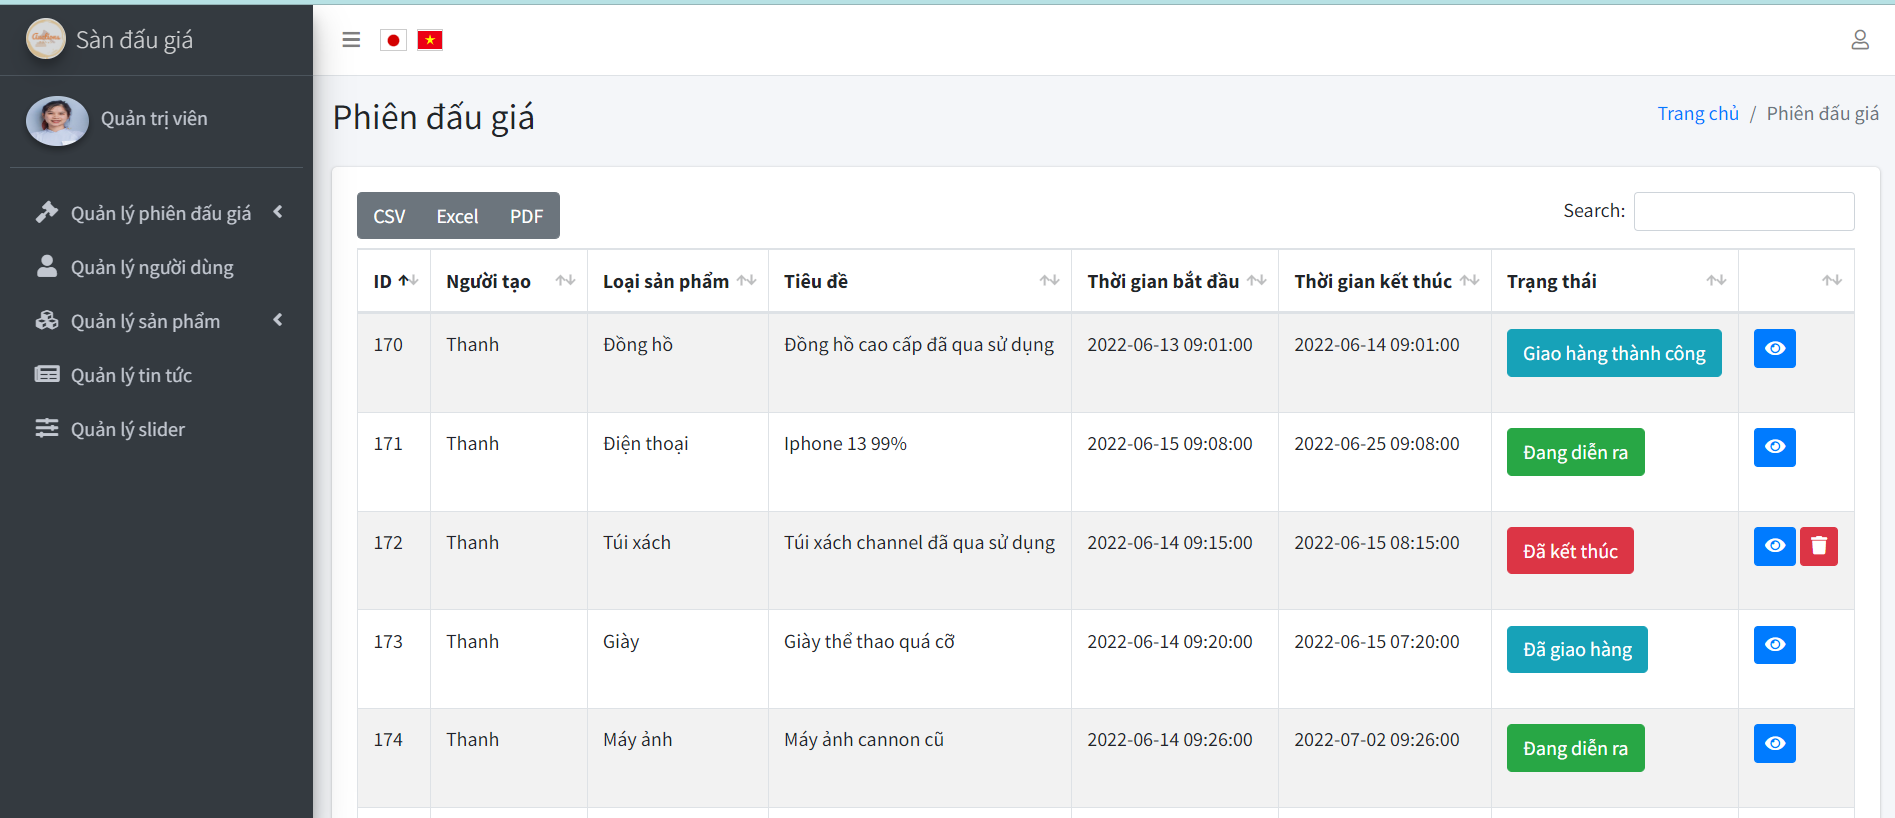
\includegraphics[width=11.4cm,height=5.0cm]{images/adminmanager.png}
\end{figure}
Quy trình đánh giá một phiên đấu giá\\
Quản trị viên có thể xem thông tin phiên đấu giá vừa được người dùng tạo
\begin{figure}[H]
    \centering
    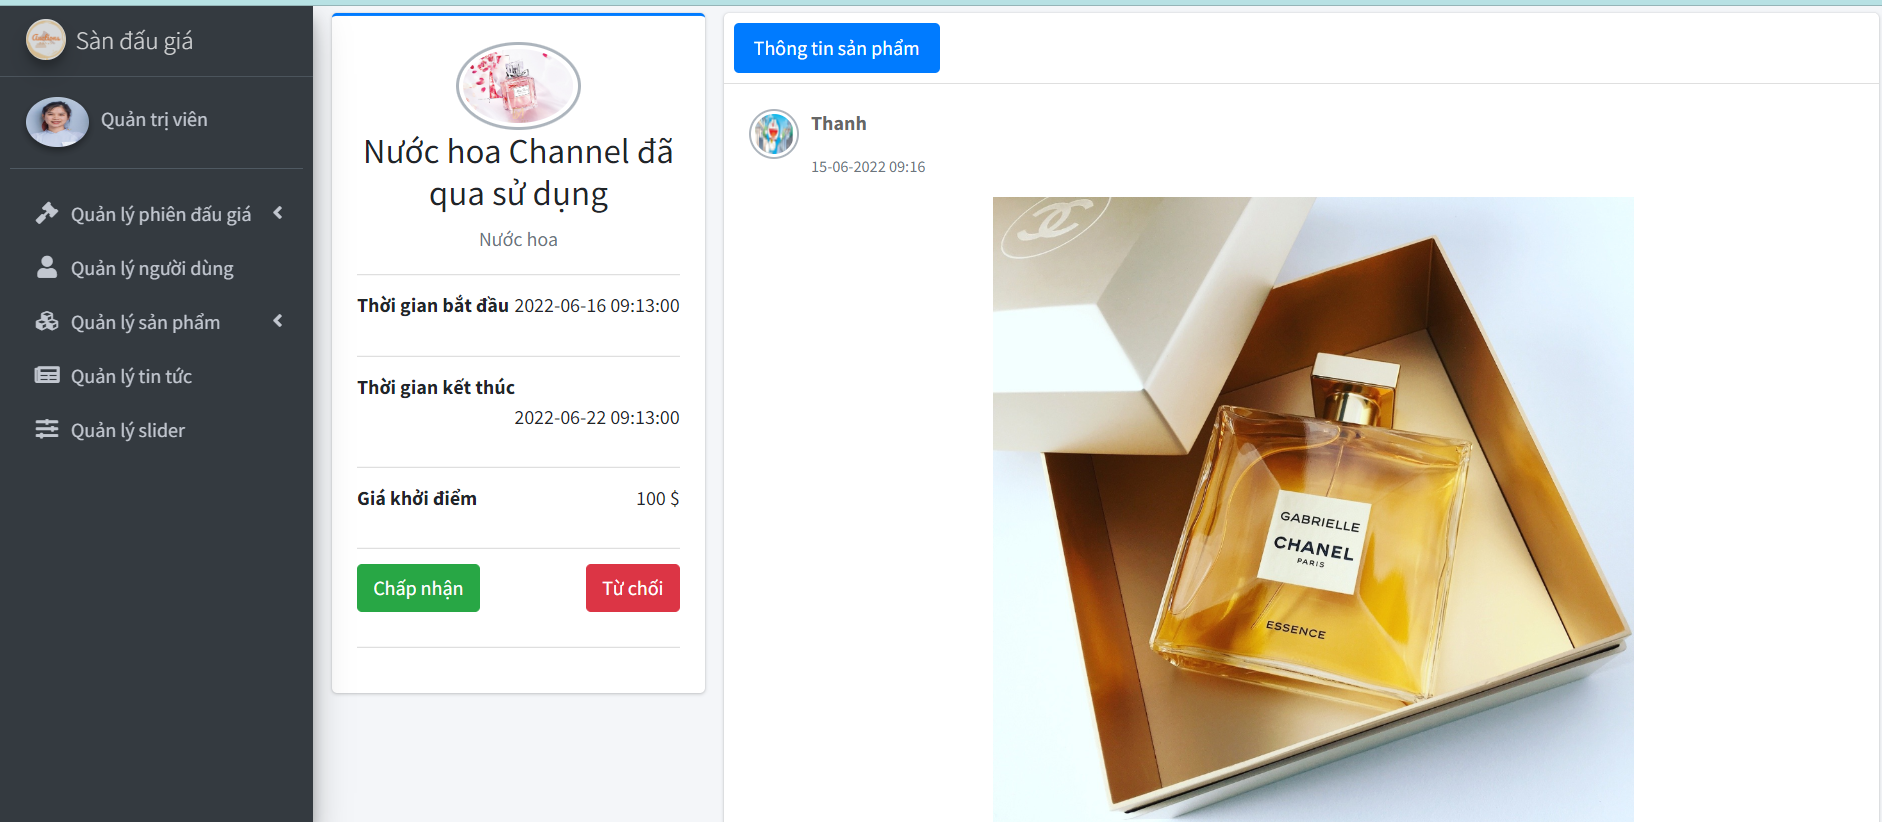
\includegraphics[width=11.4cm,height=4.96cm]{images/adminconfirm.png}
\end{figure}
Nhập đầy đủ lý do khi muốn từ chối một phiên đấu giá và chuyển thông báo đến người tạo phiên đấu giá.
\begin{figure}[H]
    \centering
    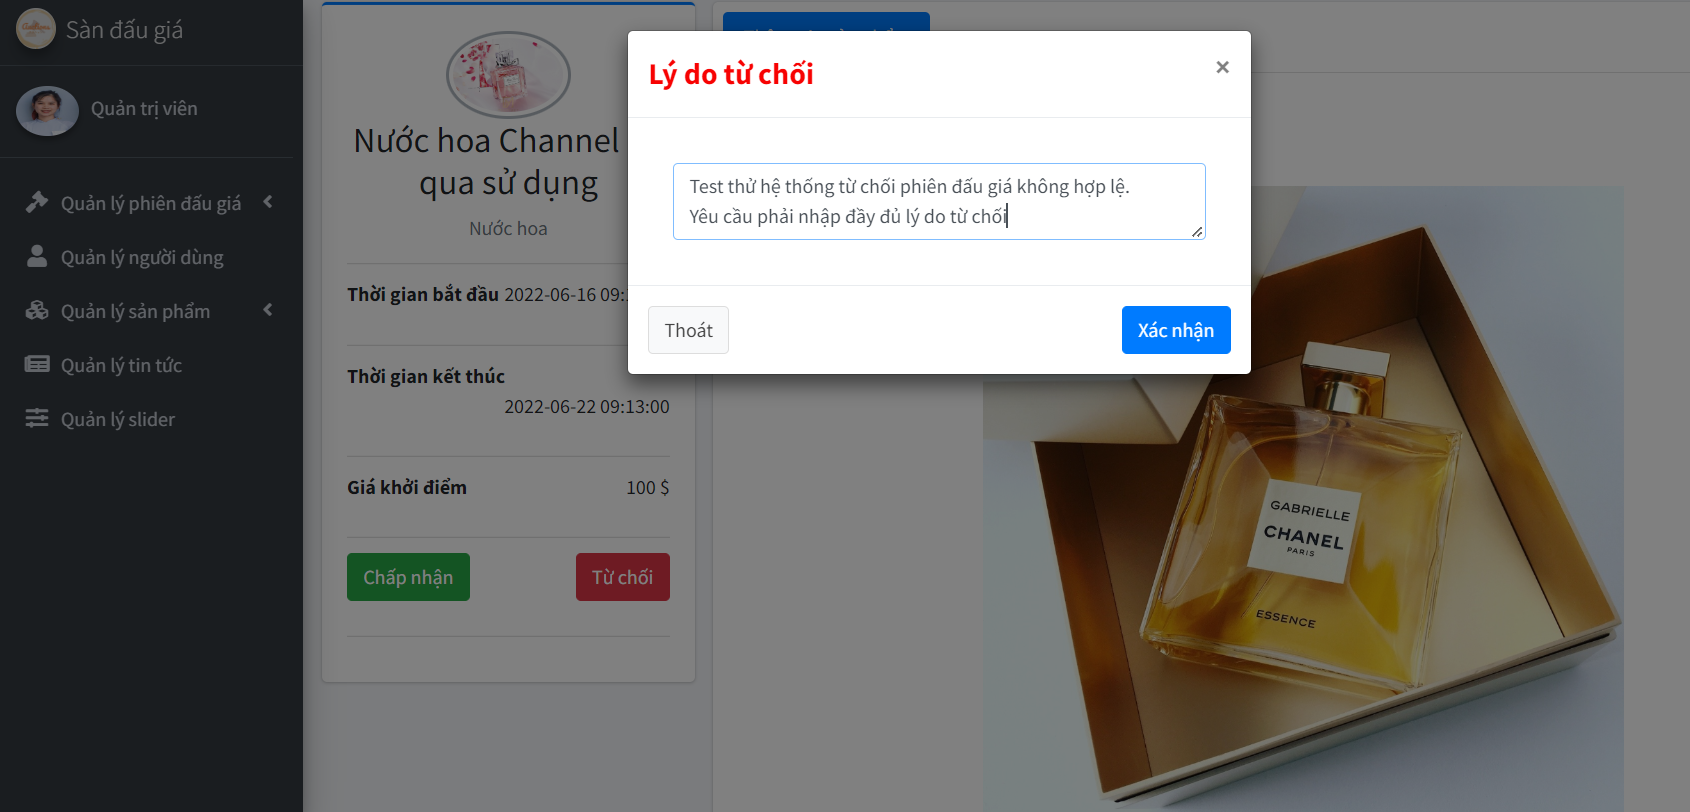
\includegraphics[width=11.4cm,height=4.83cm]{images/adminreject.png}
\end{figure}
\subsection{Hệ thống hỗ trợ người dùng có thể tìm kiếm phiên đấu giá theo nhiều tiêu chí}
\subsubsection{Đặt vấn đề}
Khi hệ thống có nhiều dữ liệu hơn thì việc tìm kiếm một phiên đấu giá phù hợp với nhu cầu của người dùng là mất rất nhiều thời gian. Thay vì việc phải lướt từ trên xuống dưới, vào xem chi tiết từng phiên đấu giá để tìm kiếm phiên đấu giá phù hợp với mình thì chức năng tìm kiếm là một giải pháp hữu ích cho người dùng.
\subsubsection{Giải pháp và kết quả đạt được}
Để giải quyết vấn đề trên thì em có tham khảo một số sàn đấu giá nổi tiếng, xem cách tìm kiếm phiên đấu giá của các website đó được tổ chức như thế nào. Bên cạnh đó để hệ thống phù hợp với người dùng nhất thì em có hỏi một số ý kiến người dùng về việc khi tìm kiếm thì người ta quan tâm đến gì nhất, thì hầu hết đều tập trung vào tên phiên đấu giá, thời gian bắt đầu, thời gian kết thúc và giá khởi điểm. \\
Áp dụng vào website đấu giá trực tuyến, nhằm vừa giảm thiểu số dữ liệu mà hệ thống phải duyệt qua để tìm kiếm và trả về thông tin mà người dùng quan tâm thì em lựa chọn sẽ tìm kiếm phiên đấu giá theo từng trạng thái và nhóm từ khóa mà người quan tâm như giá khởi điểm, thời gian diễn ra, thời gian kết thúc, tên của phiên đấu giá. \\
Dưới đây là một số hình ảnh, kết quả của việc tìm kiếm.\\
Hình ảnh kết quả tìm kiếm theo thời gian bắt đầu.
\begin{figure}[H]
    \centering
    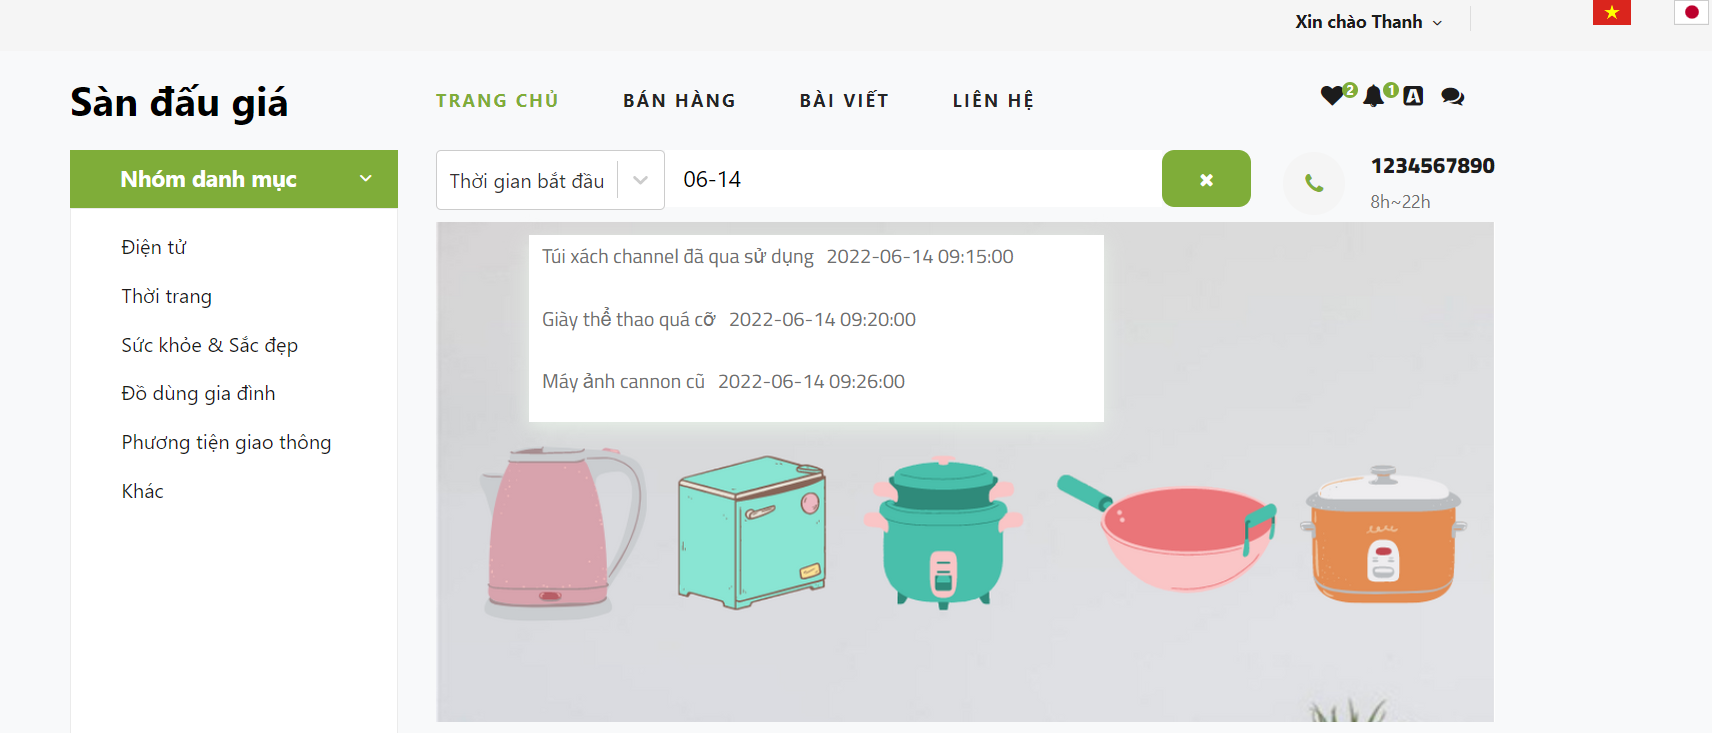
\includegraphics[width=11.4cm,height=4.89cm]{images/searchstartime.png}
\end{figure}
Ở đây người dùng muốn tìm phiên đấu giá nào có thời gian bắt đầu vào ngày 14 tháng 6. Khi đó hệ thống sẽ hiển thị tên phiên đấu giá và thời gian liên quan mà người dùng tìm kiếm. Nếu kết quả tìm kiếm nhiều thì trên màn hình chỉ hiển thị tối đa 3 phiên đấu giá theo thứ tự thời gian tăng dần, người dùng có thể dùng chuột kéo xuống dưới để thấy các kết quả khác. 
(Hình ảnh tìm kiếm phiên đấu giá theo giá khởi điểm)
\begin{figure}[H]
    \centering
    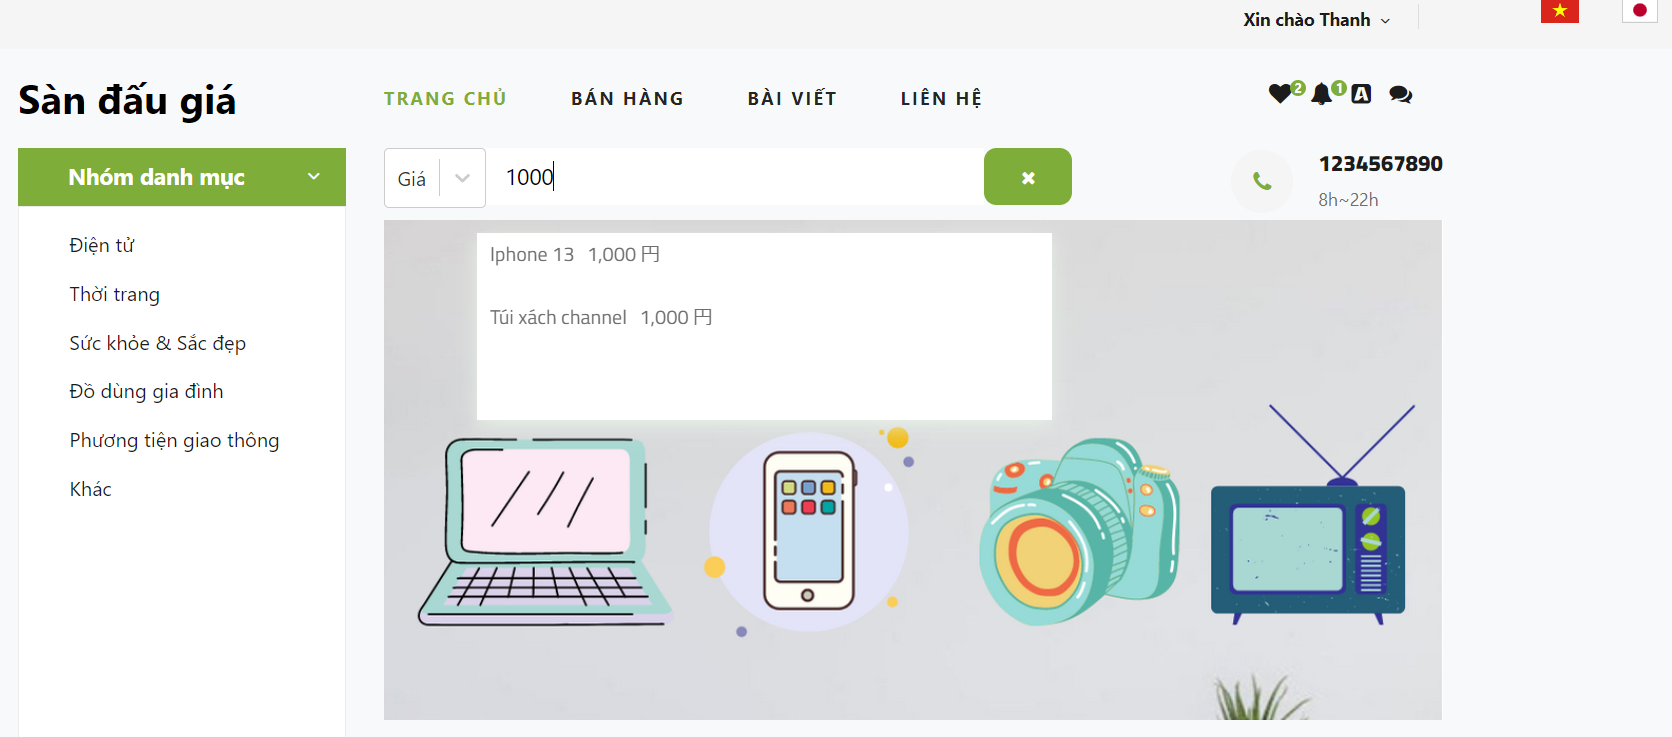
\includegraphics[width=11.4cm,height=4.82cm]{images/searchprice.png}
\end{figure}
Hình trên là tìm kiếm phiên đấu giá theo giá khởi điểm là 1000\$. Hệ thống trả ra 2 kết quả tìm được bao gồm tên phiên đấu giá và giá khởi điểm.
Ngoài việc tìm kiếm trên toàn hệ thống theo từng nhóm từ khóa, thì ở các danh sách phiên đấu giá đã được chia theo nhóm trạng thái thì cũng có thanh tìm kiếm theo tên, theo thời gian bắt đầu, kết thúc của phiên đấu giá. 
\begin{figure}[H]
    \centering
    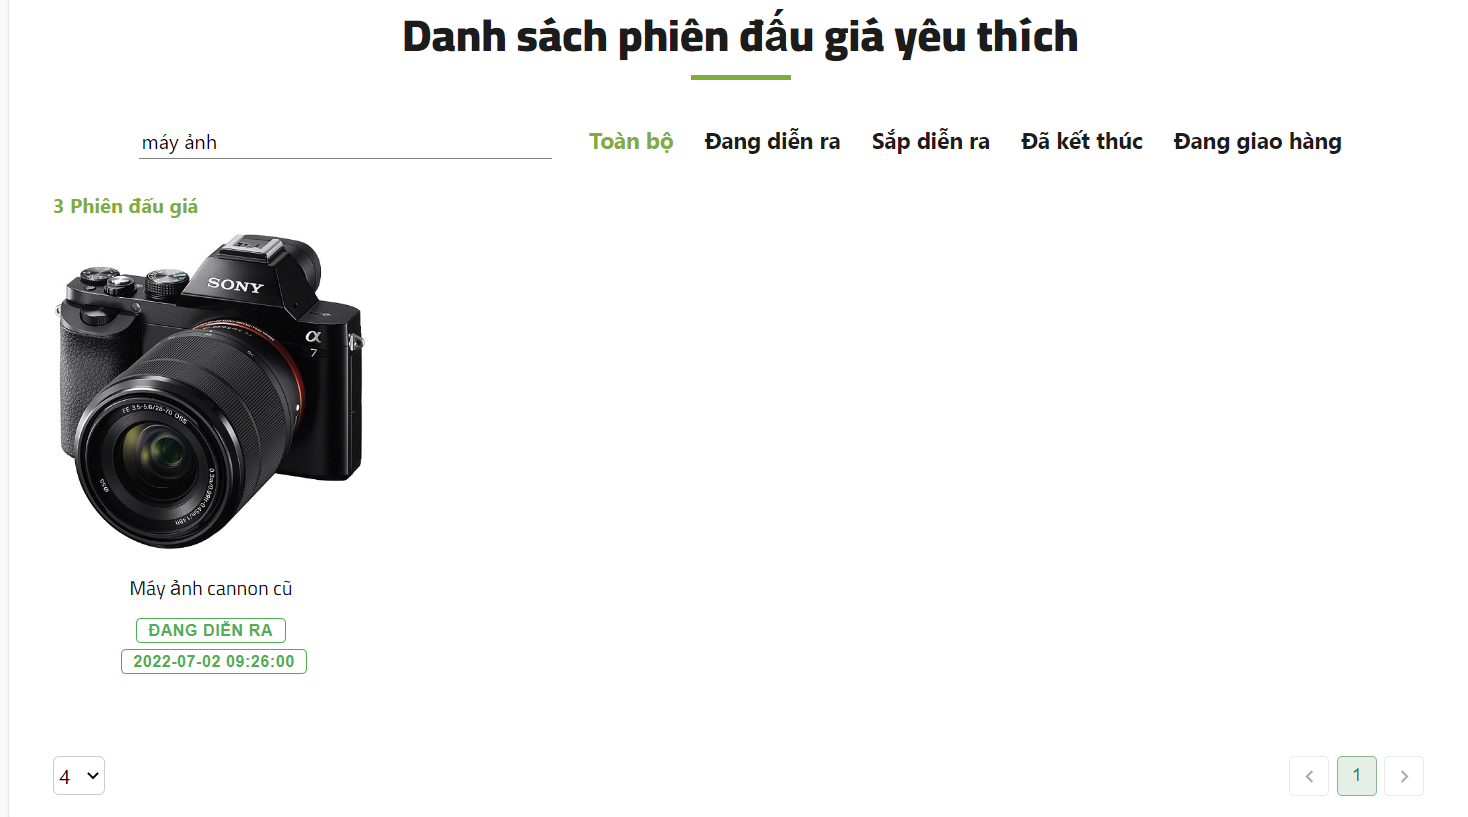
\includegraphics[width=11.4cm,height=6.36cm]{images/searchlike.png}
\end{figure}
Hình ảnh tìm kiếm phiên đấu giá tại danh sách phiên đấu giá được yêu thích (tại các danh sách phiên đấu giá khác cũng tìm kiếm tương tự)
\subsection{Hệ thống hỗ trợ nhắn tin trực tuyến}
\subsubsection{Đặt vấn đề}
Trong quá trình người dùng tham gia đấu giá hay lúc tạo phiên đấu giá, thì vấn đề thắc mắc diễn ra khá thường xuyên.  Nếu chỉ gửi email đợi phía Quản trị viên trả lời thì mất rất nhiều thời gian và khả năng bị trôi email là rất cao hoặc giải pháp bình luận trên phiên đấu giá thì cuộc hội thoại không được liền mạch và rất khó nắm bắt nội dung vì có rất nhiều người bình luận cùng một lúc khiến nội dung bình luận bị trôi. Vì vậy để thuận tiện cho việc trao đổi thông tin, thắc mắc về phiên đấu giá với Quản trị viên hay với người dùng khác thì việc có một ứng dụng nhắn tin trực tuyến là vô cùng cần thiết. 
\subsubsection{Giải pháp và kết quả đạt được}
Để giải quyết vấn đề trên thì em có tham khảo một số sàn đấu giá hiện nay thì có một số sàn liên kết với các ứng dụng nhắn tin phổ biến như Zalo, Line,.. để liên lạc. Tuy nhiên hiện tại chỉ có người dùng liên lạc với Quản trị viên đã được cài đặt mặc định. Để giải quyết thêm vấn đề có thể trao đổi, liên lạc với các người dùng khác trong website thì em đã quyết định xây dựng một ứng dụng chat sử dụng Socket.IO để đảm bảo tính realtime cho ứng dụng.\\ 
Sau đây là một số hình ảnh nhắn tin trên ứng dụng giữa người dùng với người dùng, giữa người dùng với quản trị viên. \\
Hình ảnh nhắn tin trực tuyến giữa hai người dùng
\begin{figure}[H]
    \centering
    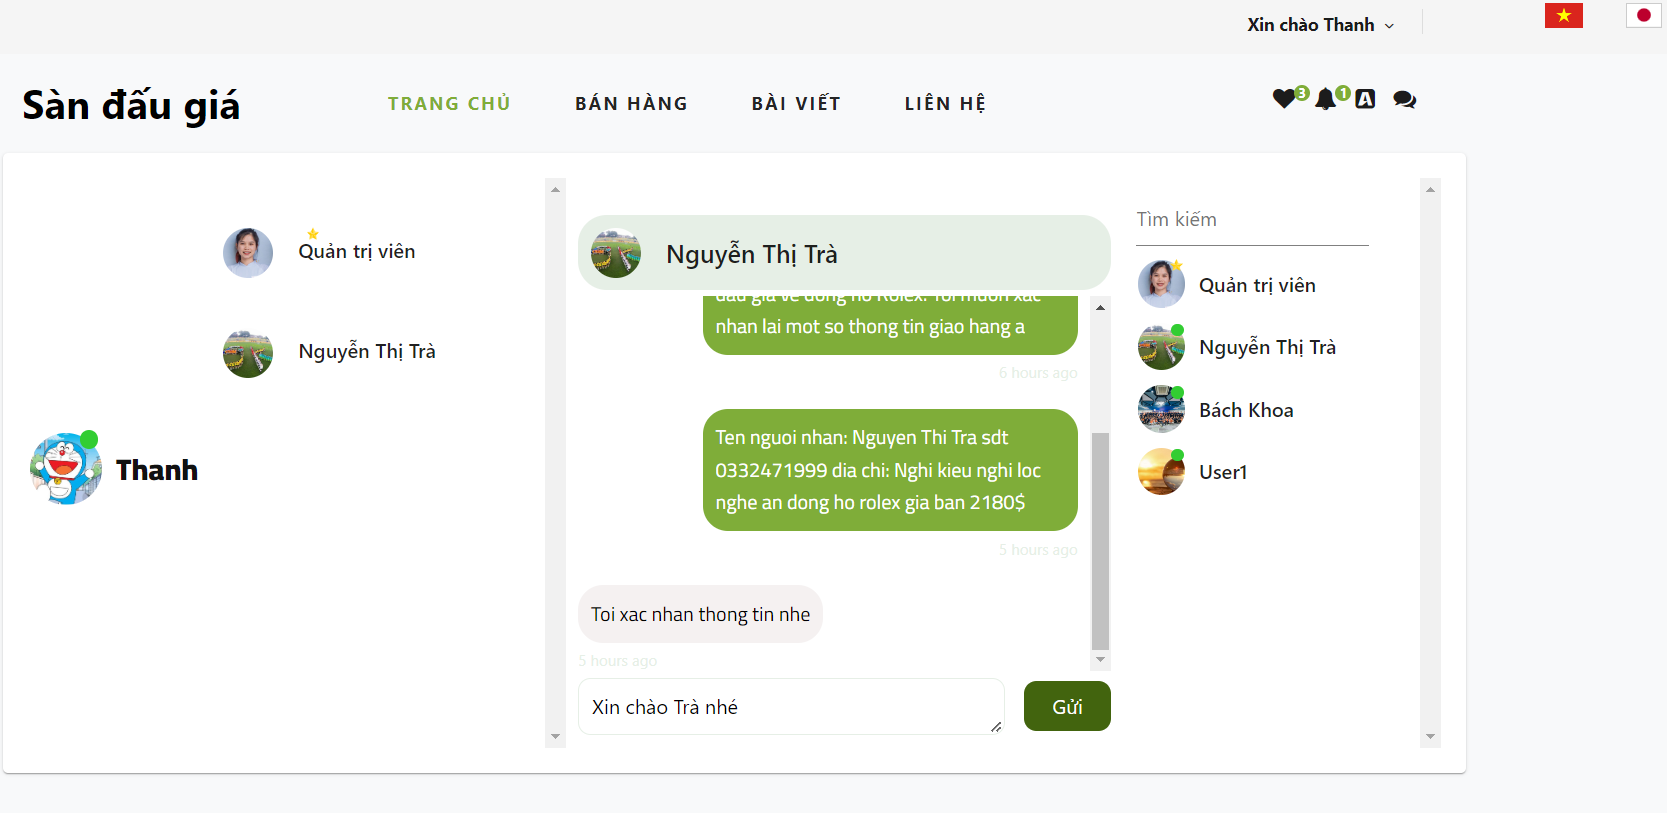
\includegraphics[width=11.4cm,height=5.55cm]{images/chatuser.png}
\end{figure}
Hình ảnh nhắn tin trực tuyến với Quản trị viên
\begin{figure}[H]
    \centering
    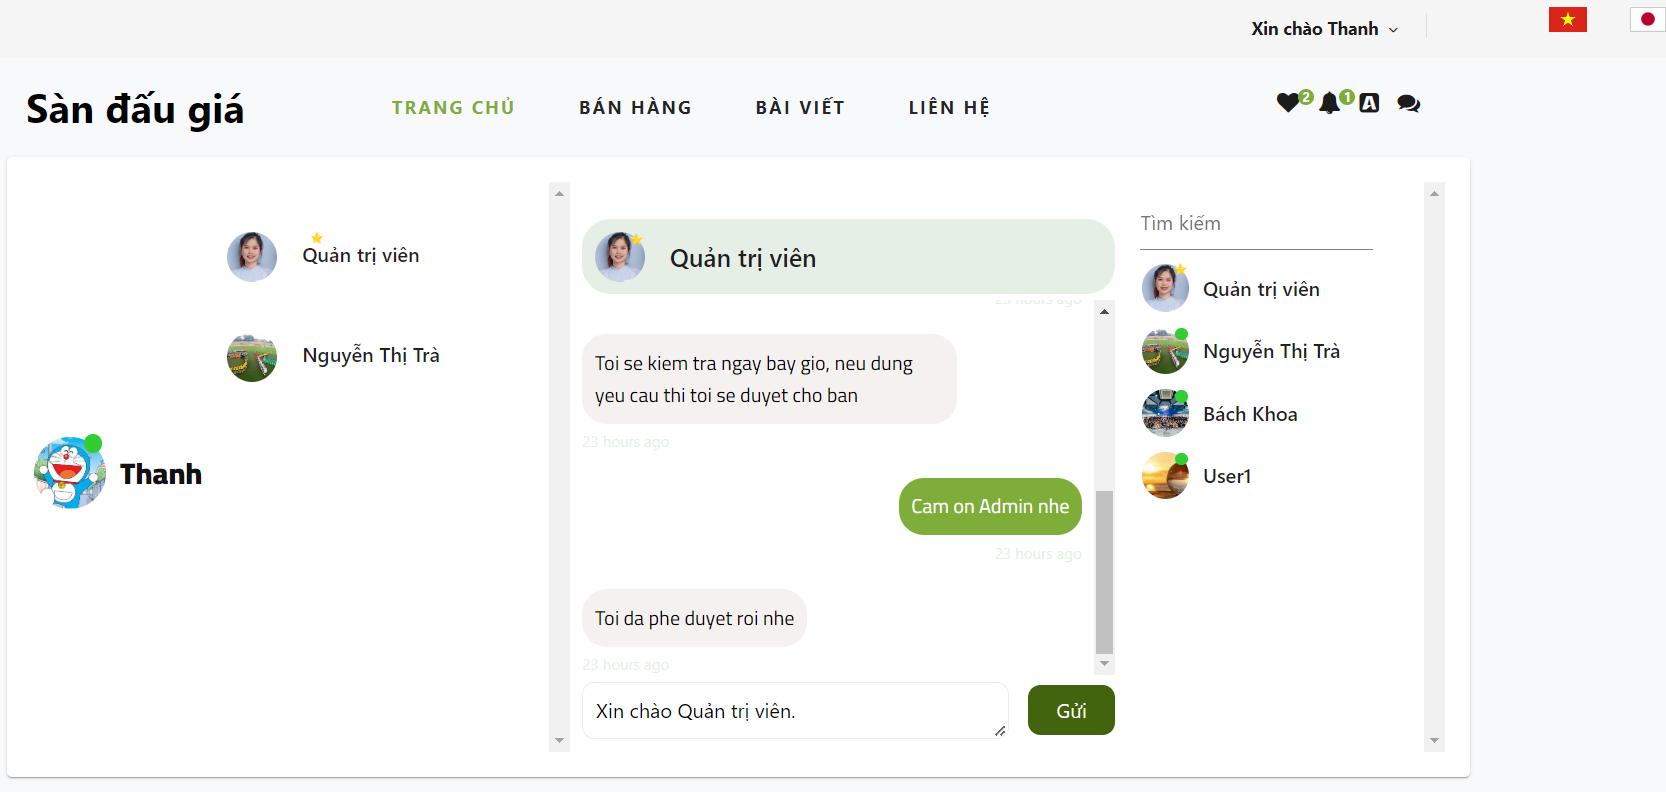
\includegraphics[width=11.4cm,height=5.42cm]{images/chatadmin.png}
\end{figure}
Để phân biệt giữa Quản trị viên và người dùng bình thường thì với tài khoản Quản trị viên sẽ có ngôi sao ở avatar.
\subsection{Hệ thống cho phép người mua đánh giá khi nhận hàng}
\subsubsection{Đặt vấn đề}
Hiện tại thì phiên đấu giá hầu như chỉ diễn ra một lần, sau khi bán sản phẩm đó thì người bán sẽ rất ít khi bán lại sản phẩm đó. Tuy nhiên việc có thêm đánh giá của người trả giá cao nhất giúp các người dùng khác nhìn nhận về người bán hàng này một cách khách quan nào đó. Dựa trên đánh giá của người nhận hàng, các người dùng khác có thể nhìn nhận khách quan rằng là người này bán hàng có uy tín không, phiên đấu giá có được thực hiện như quy định không hay sản phẩm có được như mô tả không. Những đánh giá cơ bản đó giúp cho người dùng khác quyết định có nên tham gia phiên đấu giá của người này hay không. Vì vậy việc đánh giá sau khi nhận hàng của phiên đấu giá là rất cần thiết. 
\subsubsection{Giải pháp và kết quả đạt được}
Giống như các phần mềm thương mại điện tử hiện có thì việc đánh giá được thực hiện sau khi người mua nhận được hàng. Đánh giá thì cần có ít nhất 3 yếu tố là nội dung đánh giá, số sao đánh giá và hình ảnh sản phẩm liên quan. Để chắc chắn người mua luôn phải đánh giá sản phẩm thì sau khi phía giao hàng xác nhận là đã giao hàng, thì tại giao diện phía người mua sẽ xuất hiện nút xác nhận đã nhận được hàng. Để xác nhận thì người mua bắt buộc phải thực hiện đánh giá, nếu không nhập đủ thông tin thì hệ thống sẽ báo lỗi cho đến khi người mua nhập đủ thông tin hợp lệ. Sau đó đánh giá này sẽ được hiển thị công khai trên phiên đấu giá đó để người dùng khác có thể đọc.\\
Hình ảnh form đánh giá khi người mua xác nhận đã nhận được hàng.
\begin{figure}[H]
    \centering
    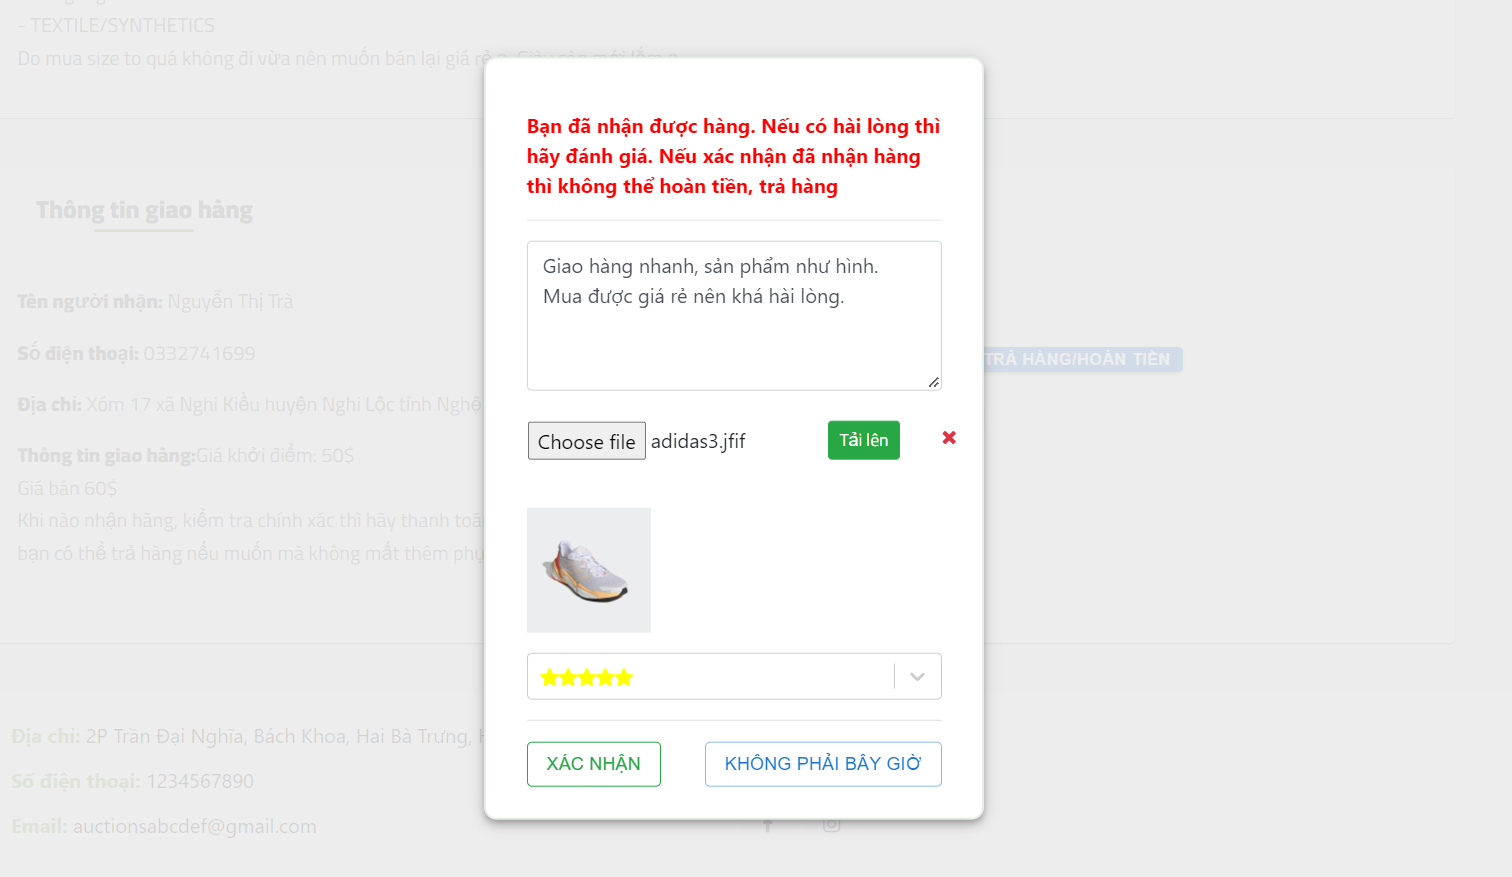
\includegraphics[width=11.4cm,height=6.62cm]{images/rate.png}
\end{figure}
Hình ảnh đánh giá được công khai lên trên giao diện phiên đấu giá
\begin{figure}[H]
    \centering
    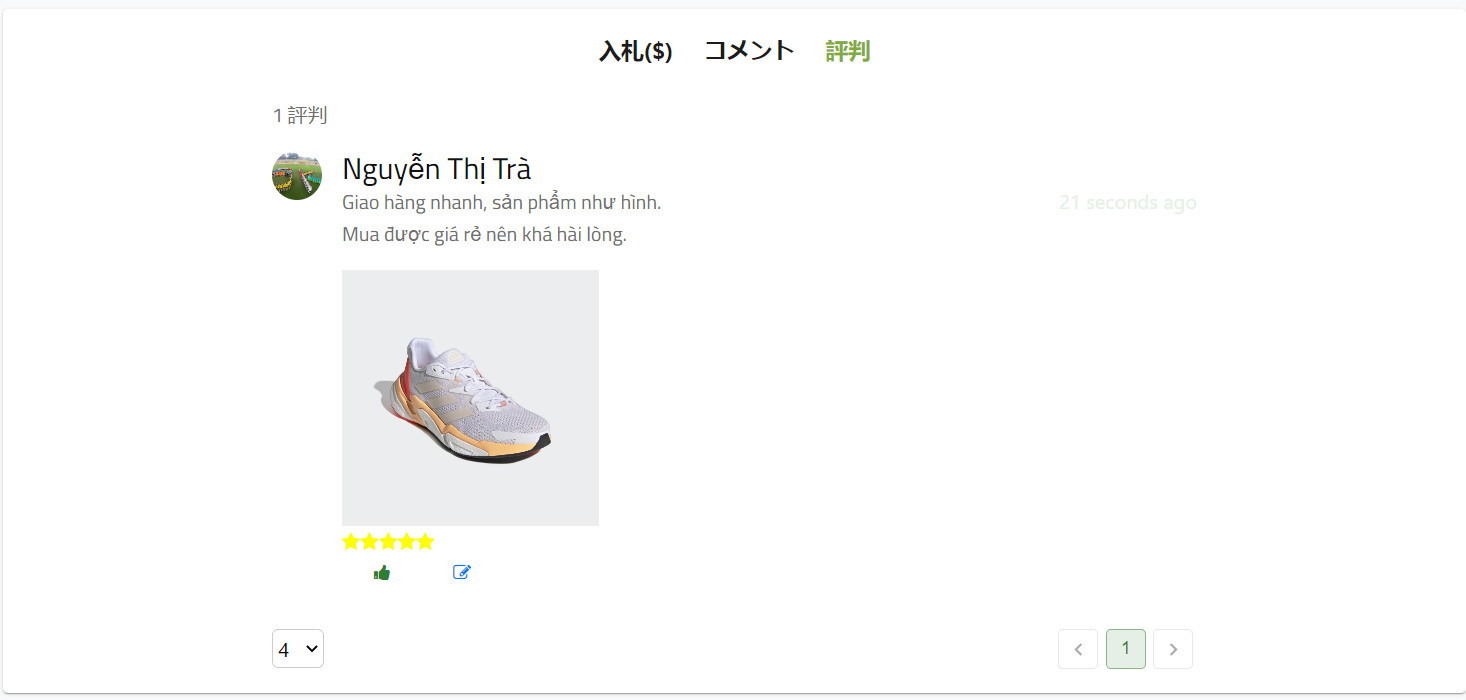
\includegraphics[width=11.4cm,height=5.46cm]{images/listrate.png}
\end{figure}
\newpage
\section*{CHƯƠNG 6 KẾT LUẬN VÀ HƯỚNG PHÁT TRIỂN}
\addcontentsline{toc}{section}{\numberline{}CHƯƠNG 6 KẾT LUẬN VÀ HƯỚNG PHÁT TRIỂN}
\setcounter{section}{6}
\setcounter{subsection}{0}
\subsection{Kết luận}
Sau một khoảng thời gian thực hiện, em đã hoàn thành ứng dụng của mình với các nhóm chức năng chính như: i) Chức năng liên quan đến tạo phiên đấu giá, ii) chức năng tham gia, đánh giá phiên đấu giá, iii) chức năng quản lý hệ thống của Quản trị viên. Mục đích chính của website là giúp người dùng có một môi trường trao đổi, buôn bán các sản phẩm với giá rẻ hơn. \\
Để so sánh với các website, sàn đấu giá hiện có thì có một số chức năng của em chưa được hoàn thiện. Tuy nhiên ứng dụng của em cũng giải quyết được vấn đề mà các ứng dụng, sàn đấu giá hiện nay không có. So với sàn đấu giá ở Việt Nam thì ứng dụng của em giải quyết được vấn đề nhắn tin trực tuyến với các tài khoản trong hệ thống, có thể đánh giá sản phẩm sau khi nhận hàng, chức năng tìm kiếm cũng tiếp cận với mong muốn người dùng hơn cùng với hệ thống quản lý bao quát, minh bạch, rõ ràng. Ngoài ra hệ thống không chỉ hướng tới nhóm người Việt Nam mà còn dành cho người Nhật Bản ở Việt Nam.\\
Tuy nhiên hệ thống vẫn còn tồn tại nhiều khuyết điểm. Về giao diện thì ở một số màn hình việc hiển thị còn chậm hơn, chức năng nhắn tin thỉnh thoảng sẽ xuất hiện lỗi là không nhắn tin được, phải reload lại ứng dụng, vẫn chưa ứng dụng được tính realtime trong quá trình đấu giá. Các chức năng cần có nhiều thời gian hơn để hoàn thiện tốt hơn.
\subsection{Hướng phát triển}
Vì thời gian xây dựng và phát triển đồ án có giới hạn nên số lượng các chức năng mà mức độ chi tiết, chính xác của từng chức năng vẫn còn hạn chế. \\
Nếu có thời gian phát triển ứng dụng trong tương lai thì đầu tiên em muốn hoàn thành việc ứng dụng realtime không chỉ ở phần nhắn tin mà còn là toàn hệ thống, đặc biệt là quá trình diễn ra đấu giá, và có thể đưa ứng dụng nhắn tin trong lúc phiên đấu giá diễn ra để người dùng có thể trao đổi với nhau. \\
Ngoài ra hiện tại tất cả người dùng có tài khoản đều có thể thực hiện bán sản phẩm, tổ chức phiên đấu giá. Vì thế trong tương lai để đảm bảo kinh phí duy trì cho website thì em mong muốn phát triển thêm chức năng tính phí cho những tài khoản muốn bán hàng, tổ chức phiên đấu giá. Thêm vào đó là chức năng liên kết với các tài khoản ngân hàng, các bên vận chuyển để thực hiện quá trình giao hàng, thanh toán được thực hiện nhanh chóng, tiện lợi hơn. 
\newpage
\section*{TÀI LIỆU THAM KHẢO}
\addcontentsline{toc}{section}{\numberline{}TÀI LIỆU THAM KHẢO}
\newpage
\section*{PHỤ LỤC}
\addcontentsline{toc}{section}{\numberline{}PHỤ LỤC}
\end{document}
